% Options for packages loaded elsewhere
\PassOptionsToPackage{unicode}{hyperref}
\PassOptionsToPackage{hyphens}{url}
\PassOptionsToPackage{dvipsnames,svgnames,x11names}{xcolor}
%
\documentclass[
  letterpaper,
  DIV=11,
  numbers=noendperiod]{scrreprt}

\usepackage{amsmath,amssymb}
\usepackage{iftex}
\ifPDFTeX
  \usepackage[T1]{fontenc}
  \usepackage[utf8]{inputenc}
  \usepackage{textcomp} % provide euro and other symbols
\else % if luatex or xetex
  \usepackage{unicode-math}
  \defaultfontfeatures{Scale=MatchLowercase}
  \defaultfontfeatures[\rmfamily]{Ligatures=TeX,Scale=1}
\fi
\usepackage{lmodern}
\ifPDFTeX\else  
    % xetex/luatex font selection
\fi
% Use upquote if available, for straight quotes in verbatim environments
\IfFileExists{upquote.sty}{\usepackage{upquote}}{}
\IfFileExists{microtype.sty}{% use microtype if available
  \usepackage[]{microtype}
  \UseMicrotypeSet[protrusion]{basicmath} % disable protrusion for tt fonts
}{}
\makeatletter
\@ifundefined{KOMAClassName}{% if non-KOMA class
  \IfFileExists{parskip.sty}{%
    \usepackage{parskip}
  }{% else
    \setlength{\parindent}{0pt}
    \setlength{\parskip}{6pt plus 2pt minus 1pt}}
}{% if KOMA class
  \KOMAoptions{parskip=half}}
\makeatother
\usepackage{xcolor}
\setlength{\emergencystretch}{3em} % prevent overfull lines
\setcounter{secnumdepth}{5}
% Make \paragraph and \subparagraph free-standing
\makeatletter
\ifx\paragraph\undefined\else
  \let\oldparagraph\paragraph
  \renewcommand{\paragraph}{
    \@ifstar
      \xxxParagraphStar
      \xxxParagraphNoStar
  }
  \newcommand{\xxxParagraphStar}[1]{\oldparagraph*{#1}\mbox{}}
  \newcommand{\xxxParagraphNoStar}[1]{\oldparagraph{#1}\mbox{}}
\fi
\ifx\subparagraph\undefined\else
  \let\oldsubparagraph\subparagraph
  \renewcommand{\subparagraph}{
    \@ifstar
      \xxxSubParagraphStar
      \xxxSubParagraphNoStar
  }
  \newcommand{\xxxSubParagraphStar}[1]{\oldsubparagraph*{#1}\mbox{}}
  \newcommand{\xxxSubParagraphNoStar}[1]{\oldsubparagraph{#1}\mbox{}}
\fi
\makeatother

\usepackage{color}
\usepackage{fancyvrb}
\newcommand{\VerbBar}{|}
\newcommand{\VERB}{\Verb[commandchars=\\\{\}]}
\DefineVerbatimEnvironment{Highlighting}{Verbatim}{commandchars=\\\{\}}
% Add ',fontsize=\small' for more characters per line
\usepackage{framed}
\definecolor{shadecolor}{RGB}{241,243,245}
\newenvironment{Shaded}{\begin{snugshade}}{\end{snugshade}}
\newcommand{\AlertTok}[1]{\textcolor[rgb]{0.68,0.00,0.00}{#1}}
\newcommand{\AnnotationTok}[1]{\textcolor[rgb]{0.37,0.37,0.37}{#1}}
\newcommand{\AttributeTok}[1]{\textcolor[rgb]{0.40,0.45,0.13}{#1}}
\newcommand{\BaseNTok}[1]{\textcolor[rgb]{0.68,0.00,0.00}{#1}}
\newcommand{\BuiltInTok}[1]{\textcolor[rgb]{0.00,0.23,0.31}{#1}}
\newcommand{\CharTok}[1]{\textcolor[rgb]{0.13,0.47,0.30}{#1}}
\newcommand{\CommentTok}[1]{\textcolor[rgb]{0.37,0.37,0.37}{#1}}
\newcommand{\CommentVarTok}[1]{\textcolor[rgb]{0.37,0.37,0.37}{\textit{#1}}}
\newcommand{\ConstantTok}[1]{\textcolor[rgb]{0.56,0.35,0.01}{#1}}
\newcommand{\ControlFlowTok}[1]{\textcolor[rgb]{0.00,0.23,0.31}{\textbf{#1}}}
\newcommand{\DataTypeTok}[1]{\textcolor[rgb]{0.68,0.00,0.00}{#1}}
\newcommand{\DecValTok}[1]{\textcolor[rgb]{0.68,0.00,0.00}{#1}}
\newcommand{\DocumentationTok}[1]{\textcolor[rgb]{0.37,0.37,0.37}{\textit{#1}}}
\newcommand{\ErrorTok}[1]{\textcolor[rgb]{0.68,0.00,0.00}{#1}}
\newcommand{\ExtensionTok}[1]{\textcolor[rgb]{0.00,0.23,0.31}{#1}}
\newcommand{\FloatTok}[1]{\textcolor[rgb]{0.68,0.00,0.00}{#1}}
\newcommand{\FunctionTok}[1]{\textcolor[rgb]{0.28,0.35,0.67}{#1}}
\newcommand{\ImportTok}[1]{\textcolor[rgb]{0.00,0.46,0.62}{#1}}
\newcommand{\InformationTok}[1]{\textcolor[rgb]{0.37,0.37,0.37}{#1}}
\newcommand{\KeywordTok}[1]{\textcolor[rgb]{0.00,0.23,0.31}{\textbf{#1}}}
\newcommand{\NormalTok}[1]{\textcolor[rgb]{0.00,0.23,0.31}{#1}}
\newcommand{\OperatorTok}[1]{\textcolor[rgb]{0.37,0.37,0.37}{#1}}
\newcommand{\OtherTok}[1]{\textcolor[rgb]{0.00,0.23,0.31}{#1}}
\newcommand{\PreprocessorTok}[1]{\textcolor[rgb]{0.68,0.00,0.00}{#1}}
\newcommand{\RegionMarkerTok}[1]{\textcolor[rgb]{0.00,0.23,0.31}{#1}}
\newcommand{\SpecialCharTok}[1]{\textcolor[rgb]{0.37,0.37,0.37}{#1}}
\newcommand{\SpecialStringTok}[1]{\textcolor[rgb]{0.13,0.47,0.30}{#1}}
\newcommand{\StringTok}[1]{\textcolor[rgb]{0.13,0.47,0.30}{#1}}
\newcommand{\VariableTok}[1]{\textcolor[rgb]{0.07,0.07,0.07}{#1}}
\newcommand{\VerbatimStringTok}[1]{\textcolor[rgb]{0.13,0.47,0.30}{#1}}
\newcommand{\WarningTok}[1]{\textcolor[rgb]{0.37,0.37,0.37}{\textit{#1}}}

\providecommand{\tightlist}{%
  \setlength{\itemsep}{0pt}\setlength{\parskip}{0pt}}\usepackage{longtable,booktabs,array}
\usepackage{calc} % for calculating minipage widths
% Correct order of tables after \paragraph or \subparagraph
\usepackage{etoolbox}
\makeatletter
\patchcmd\longtable{\par}{\if@noskipsec\mbox{}\fi\par}{}{}
\makeatother
% Allow footnotes in longtable head/foot
\IfFileExists{footnotehyper.sty}{\usepackage{footnotehyper}}{\usepackage{footnote}}
\makesavenoteenv{longtable}
\usepackage{graphicx}
\makeatletter
\def\maxwidth{\ifdim\Gin@nat@width>\linewidth\linewidth\else\Gin@nat@width\fi}
\def\maxheight{\ifdim\Gin@nat@height>\textheight\textheight\else\Gin@nat@height\fi}
\makeatother
% Scale images if necessary, so that they will not overflow the page
% margins by default, and it is still possible to overwrite the defaults
% using explicit options in \includegraphics[width, height, ...]{}
\setkeys{Gin}{width=\maxwidth,height=\maxheight,keepaspectratio}
% Set default figure placement to htbp
\makeatletter
\def\fps@figure{htbp}
\makeatother
% definitions for citeproc citations
\NewDocumentCommand\citeproctext{}{}
\NewDocumentCommand\citeproc{mm}{%
  \begingroup\def\citeproctext{#2}\cite{#1}\endgroup}
\makeatletter
 % allow citations to break across lines
 \let\@cite@ofmt\@firstofone
 % avoid brackets around text for \cite:
 \def\@biblabel#1{}
 \def\@cite#1#2{{#1\if@tempswa , #2\fi}}
\makeatother
\newlength{\cslhangindent}
\setlength{\cslhangindent}{1.5em}
\newlength{\csllabelwidth}
\setlength{\csllabelwidth}{3em}
\newenvironment{CSLReferences}[2] % #1 hanging-indent, #2 entry-spacing
 {\begin{list}{}{%
  \setlength{\itemindent}{0pt}
  \setlength{\leftmargin}{0pt}
  \setlength{\parsep}{0pt}
  % turn on hanging indent if param 1 is 1
  \ifodd #1
   \setlength{\leftmargin}{\cslhangindent}
   \setlength{\itemindent}{-1\cslhangindent}
  \fi
  % set entry spacing
  \setlength{\itemsep}{#2\baselineskip}}}
 {\end{list}}
\usepackage{calc}
\newcommand{\CSLBlock}[1]{\hfill\break\parbox[t]{\linewidth}{\strut\ignorespaces#1\strut}}
\newcommand{\CSLLeftMargin}[1]{\parbox[t]{\csllabelwidth}{\strut#1\strut}}
\newcommand{\CSLRightInline}[1]{\parbox[t]{\linewidth - \csllabelwidth}{\strut#1\strut}}
\newcommand{\CSLIndent}[1]{\hspace{\cslhangindent}#1}

\usepackage{booktabs}
\usepackage{longtable}
\usepackage{array}
\usepackage{multirow}
\usepackage{wrapfig}
\usepackage{float}
\usepackage{colortbl}
\usepackage{pdflscape}
\usepackage{tabu}
\usepackage{threeparttable}
\usepackage{threeparttablex}
\usepackage[normalem]{ulem}
\usepackage{makecell}
\usepackage{xcolor}
\KOMAoption{captions}{tableheading}
\makeatletter
\@ifpackageloaded{bookmark}{}{\usepackage{bookmark}}
\makeatother
\makeatletter
\@ifpackageloaded{caption}{}{\usepackage{caption}}
\AtBeginDocument{%
\ifdefined\contentsname
  \renewcommand*\contentsname{Tabla de contenidos}
\else
  \newcommand\contentsname{Tabla de contenidos}
\fi
\ifdefined\listfigurename
  \renewcommand*\listfigurename{Listado de Figuras}
\else
  \newcommand\listfigurename{Listado de Figuras}
\fi
\ifdefined\listtablename
  \renewcommand*\listtablename{Listado de Tablas}
\else
  \newcommand\listtablename{Listado de Tablas}
\fi
\ifdefined\figurename
  \renewcommand*\figurename{Figura}
\else
  \newcommand\figurename{Figura}
\fi
\ifdefined\tablename
  \renewcommand*\tablename{Tabla}
\else
  \newcommand\tablename{Tabla}
\fi
}
\@ifpackageloaded{float}{}{\usepackage{float}}
\floatstyle{ruled}
\@ifundefined{c@chapter}{\newfloat{codelisting}{h}{lop}}{\newfloat{codelisting}{h}{lop}[chapter]}
\floatname{codelisting}{Listado}
\newcommand*\listoflistings{\listof{codelisting}{Listado de Listados}}
\makeatother
\makeatletter
\makeatother
\makeatletter
\@ifpackageloaded{caption}{}{\usepackage{caption}}
\@ifpackageloaded{subcaption}{}{\usepackage{subcaption}}
\makeatother

\ifLuaTeX
\usepackage[bidi=basic]{babel}
\else
\usepackage[bidi=default]{babel}
\fi
\babelprovide[main,import]{spanish}
% get rid of language-specific shorthands (see #6817):
\let\LanguageShortHands\languageshorthands
\def\languageshorthands#1{}
\ifLuaTeX
  \usepackage{selnolig}  % disable illegal ligatures
\fi
\usepackage{bookmark}

\IfFileExists{xurl.sty}{\usepackage{xurl}}{} % add URL line breaks if available
\urlstyle{same} % disable monospaced font for URLs
\hypersetup{
  pdftitle={Bitácoras Grupo \#5, CA-204 (II-2024)},
  pdfauthor={Jeikel Navarro Solis, Gabriel Valverde, Erick Venegas},
  pdflang={es},
  colorlinks=true,
  linkcolor={blue},
  filecolor={Maroon},
  citecolor={Blue},
  urlcolor={Blue},
  pdfcreator={LaTeX via pandoc}}


\title{Bitácoras Grupo \#5, CA-204 (II-2024)}
\usepackage{etoolbox}
\makeatletter
\providecommand{\subtitle}[1]{% add subtitle to \maketitle
  \apptocmd{\@title}{\par {\large #1 \par}}{}{}
}
\makeatother
\subtitle{Análisis de las variables cualitativas en relación al riesgo
crediticio alrededor del mundo}
\author{Jeikel Navarro Solis, Gabriel Valverde, Erick Venegas}
\date{2024-10-03}

\begin{document}
\maketitle

\renewcommand*\contentsname{Tabla de contenidos}
{
\hypersetup{linkcolor=}
\setcounter{tocdepth}{2}
\tableofcontents
}

\bookmarksetup{startatroot}

\chapter*{Introducción}\label{introducciuxf3n}
\addcontentsline{toc}{chapter}{Introducción}

\markboth{Introducción}{Introducción}

Este estudio utiliza una base de datos de riesgos financieros en el cual
se toman en cuanta variables como lo son la edad, genero, pais en el que
vive y estado marital de las personas, esto con el fin de realizar un
perfil descriptivo de los prestatario, asi como tambien se toman
variables cuantitativas como los ingresos, activos y deuda de la persona
en cuestion. De manera que la base contiene un total de 15000 casos y 20
variables. El objetivo es generar empiricamente un metodo que basado en
las variables permita crear una calificación de riesgo, tal que se
puedan relacionar las variables cuantitativas y cualitativas de modo tal
se logre llegar a algún resultado satisfactorio a partir de estos datos.
Por estas razones, la investigación se basa en un marco teorico y
empirico donde los autores buscan salir de la norma y explorar mas
factores que solo la parte economica de los prestatarios.

\bookmarksetup{startatroot}

\chapter{Bitacora 1}\label{bitacora-1}

\section{Parte de planificación}\label{parte-de-planificaciuxf3n}

\subsection{Definión de la idea}\label{definiuxf3n-de-la-idea}

Cuando una persona quiere acceder a un préstamo bancario, es común que
los bancos requieran información personal y profesional de la persona,
por ejemplo su profesión, ingresos mensuales, edad, gastos mensuales,
etc. Esto se debe a que los bancos necesitan saber si esta persona es
apta para pagar el préstamo en un tiempo conveniente. Generalmente se
piensa que, mientras más ingresos tenga la persona, es más probable que
le acepten el crédito a financiar. Añadido a esto, también es frecuente
escuchar que mientras la persona tenga un mayor grado académico, ésta
tendrá un mejor salario o tendrá más formas de ingresar dinero a sus
cuentas. Ante esta situación, nos surgió la idea de comprobar si estos
estereotipos son ciertos ó no. Por lo que nuestra meta es lograr
determinar si realmente el nivel de educación y el nivel de ingresos
influye en la capacidad de pago de una persona en un préstamo, así como
analizar si los factores cualitativos tienen cierta relevancia al
momento de que haya un impago.

\subsection{Conceptualización de la
idea}\label{conceptualizaciuxf3n-de-la-idea}

``Verificar una relación entre la calificación de riesgo con las
variables Nivel de educación, Ingresos, Monto del préstamo''. De la
pregunta anterior, nos interesa conceptualizar dicha idea, por lo que,
buscando la definición de las palabras que conforman la idea, en la RAE,
encontramos lo siguiente:

\begin{itemize}
\item
  Relación: Conexión, correspondencia.
\item
  Nivel: Medida de una cantidad con referencia a una escala determinada.
\item
  Educación: Acción y efecto de educar, instrucción por medio de la
  acción docente.
\item
  Ingresos: Caudal que entra en poder de alguien, y que le es de cargo
  en las cuentas.
\item
  Calificación: Puntuación obtenida en un examen o en cualquier tipo de
  prueba.
\item
  Riesgo: Contingencia o proximidad de un daño.
\end{itemize}

\subsection{Identificación de
tensiones}\label{identificaciuxf3n-de-tensiones}

Como mencionamos en el apartado anterior, el trabajo se centra más en el
estudio de las herramientas utilizadas, que en la información del
trabajo per se. Sin embargo, vamos a desarrollar la teoría de manera
satisfactoria con el hecho de crear un trabajo bien estructurado. Dicho
lo anterior, es claro que la calificación de riesgo es un fenómeno que
depende de muchas más variables, un ejemplo de ello puede ser la cultura
de la sociedad en la cual se ve inmersa la persona que solicita el
préstamo, como la entidad que lo desembolsa. Por ello, el origen de los
datos de esta tabla de datos es de suma importancia, pues la cultura de
las personas que arrojaron estos datos puede influir de manera
sustancial en la salida de los datos.

Otro factor a tomar en cuenta es por supuesto, la tabla de datos, pues
podría contener información errónea, o datos que no estén correctamente
digitados, además de que la tabla de datos tiene que ser convertida a
información más trabajable, es decir, muchas de las variables son
categóricas, por lo que una conversión a datos de diferente especie,
podría provocar que haya errores en la nueva tabla que se va a
manipular.

\subsection{Reformulación de la idea en modo
preguntas}\label{reformulaciuxf3n-de-la-idea-en-modo-preguntas}

La idea principal de este trabajo es: ``Verificar una relación entre la
calificación de riesgo con las variables Nivel de educación, Ingresos,
Monto del préstamo'', por lo que para etsa parte del trabajo, vamos a
formular la idea de diferentes formas, esto con el fin de formular una
pregunta de investigación que sea clara.

\emph{¿Cuáles son las variables que influyen más en la calificación de
riesgo? }¿Existe una correlación positiva entre las variables de interés
y la calificación de riesgo? \emph{¿Es la calificación de riesgo un buen
calificador de las variables que la determinan? }¿Cómo se mide la
calificación de riesgo dadas las variables consideradas?

\subsection{Argumentación de las
preguntas}\label{argumentaciuxf3n-de-las-preguntas}

Estas preguntas deben poseer una argumentación detrás de ellas, pues es
necesario tener una idea de qué es lo que queremos realizar con estas
preguntas o dicho de otra forma, cuál es el problema que potencialmente
podemos resolver o la incógnita a contestar.8

\subsubsection{¿Cuáles son las variables que influyen más en la
calificación de
riesgo?}\label{cuuxe1les-son-las-variables-que-influyen-muxe1s-en-la-calificaciuxf3n-de-riesgo}

\textbf{Contraargumentos}

Las variables que se toman son realmente las correctas, cuál es el
método que se utiliza para determinar que las variables que se están
tomando son mejores para un resultado que otras. Al ser una calificación
de riesgo, que facilita el préstamo a personas o no, las personas
podrían tener intenciones perversas a siempre manipular su información
para obtener buenas calificaciones. Por otro lado, son muchas las
variables contempladas en la base de datos, hacer uso de un par de
variables, podría influir de manera considerable en buscar una relación
entre las variables.

\textbf{Argumentos}

Al realizar un análisis previo de la tabla de datos, podríamos
determinar cuáles son las variables con mayor impacto en esta
calificación, y así simplificar el modelo y darle un mayor énfasis en
estas variables que afectan de manera considerable en la calificación.

\textbf{Concluya}

Al ser una calificación de riesgo, las empresas deben considerar varios
factores, para ver si sus clientes son ideales para el préstamo o no.
Por otro lado, concentrarnos en las variables que tienen mayor peso,
podría ayudar a un mejor entendimiento de la calificación de riesgo.

\subsubsection{¿Existe una correlación positiva entre las variables de
interés y la calificación de
riesgo?}\label{existe-una-correlaciuxf3n-positiva-entre-las-variables-de-interuxe9s-y-la-calificaciuxf3n-de-riesgo}

\textbf{Contraargumentos} Una relación positiva no implica que haya una
mejor calificación, pues pueden existir variables con relación negativa,
que tengan un efecto positivo sobre la calificación de riesgo, por pura
intuición, podemos pensar en las personas que tienen un récord
crediticio limpio, esto implicaría que esta variable debería tener un
valor nulo para mejorar la calificación de riesgo. Otra variable que
podría afectar es las veces que la persona ha caído en impago, pues
entre más suba este valor, la calificación de riesgo, debería ser menor.

\textbf{Argumentos}

Las relaciones que buscamos no tienen por qué ser positivas, desde un
tipo de vista de coeficiente de correlación, sino desde un tipo de vista
de mejoría, es decir, variables que en ausencia contribuyan a una mejor
calificación, nos son de interés para el trabajo. Como hemos mencionado
encontrar las relaciones más contribuyentes, son de utilidad, pues
favorecen a simplificar el modelo y obtener a cambio una mejor
interpretación del estudio.

\textbf{Concluya}

Todas las relaciones son de importancia, hasta donde no existe relación,
pues sirven para delimitar el modelo y determinar cuáles son las
verdaderas variables que si influyen.

\subsubsection{\texorpdfstring{\textbf{¿Es la calificación de riesgo un
buen calificador de las variables que la
determinan?}}{¿Es la calificación de riesgo un buen calificador de las variables que la determinan?}}\label{es-la-calificaciuxf3n-de-riesgo-un-buen-calificador-de-las-variables-que-la-determinan}

\textbf{Contraargumentos}

Esta pregunta, no es del todo objetiva, pues dependerá de lo que la
empresa quiera detectar en estas evaluaciones, es decir, un factor que
determina en gran medida a la calificación de riesgo, en otra empresa no
tiene por qué ser así, pues dependerá del público objetivo de la
empresa. Un buen calificador de riesgo depende tanto de las variables
que se toman en cuenta, como del contexto de la empresa.

\textbf{Argumentos}

Desde el punto de vista de la empresa, la calificación de riesgo es una
herramienta que sirve para determinar en gran medida si un préstamo se
realiza o no, por ello, saber si su calificación de riesgo logra captar
la información deseada de las variables utilizadas, entonces se podría
considerar un buen factor, pues, aunque las empresas deban tener cuidado
a quiénes otorgan los préstamos, también es un hecho, que si no lo
hacen, se quedan sin negocio

\textbf{Concluya}

Si la calificación de riesgo logra simplificar y consolidar la
información, entonces podríamos conjeturar que se comporta como una
buena calificación.

\subsubsection{\texorpdfstring{\textbf{¿Cómo se mide la calificación de
riesgo dadas las variables
consideradas?}}{¿Cómo se mide la calificación de riesgo dadas las variables consideradas?}}\label{cuxf3mo-se-mide-la-calificaciuxf3n-de-riesgo-dadas-las-variables-consideradas}

\textbf{Contraargumentos}

La pregunta es más compleja que las hechas anteriormente, pues estamos
entrando a un método de calificación, es decir, hacer un análisis de la
medición, como mencionamos como un contraargumento en la pregunta
anterior, esto no tiene por qué ser universal en las empresas, esto
puede variar, por lo que dependerá del contexto en el cual se realice la
pregunta.

\textbf{Argumentos}

En realidad que sea una pregunta que depende de sus variables, podría
ser beneficioso, pues si existen varias metodologías, podríamos tener
una mejor cartera de préstamos, es decir, dado cierto tipo de cliente,
se podrían realizar cierto tipo de préstamos.

\textbf{Concluya}

La subjetividad de esta pregunta, no es ni buena ni mala, esta depende
su contexto, si es aplicada de una buena forma, podría ser beneficioso
tanto para la empresa, por ampliar su mercado, como para el cliente, al
recibir el préstamo deseado.

\subsection{Argumentación a través de
datos}\label{argumentaciuxf3n-a-travuxe9s-de-datos}

La base de datos utilizada en este trabajo se toma de la base de datos
de Kaggle. Sin embargo, el autor de la base de datos no publica la
información de cuándo es sacada la información. La información fue de
fácil acceso pues está disponible en la de datos de Kaggle. La muestra
observada son personas entre las edades de 18 a 69 años, de donde toman
muchas variables, las cuales veremos más adelante. La unidad estadística
estudiada para este trabajo son individuos que buscan obtener un
préstamo.

Para la siguiente vamos a tomar el nombre las variables, las cuales
dejaremos en el idioma original y vamos a dar la descripción de ellas,
las cuales viene a su vez con la tabla de datos.

\begin{itemize}
\item
  Age: La edad del individuo, una variable continua que influye en la
  estabilidad financiera.
\item
  Gender: Género del individuo, categorizado en Masculino, Femenino y No
  binario.
\item
  Education Level: Nivel de educación alcanzado, que varía desde la
  Secundaria hasta el Doctorado.
\item
  Marital Status: Estado civil actual, categorizado como Soltero,
  Casado, Divorciado o Viudo.
\item
  Income: Ingreso anual en USD, que representa la capacidad de ganancia
  del individuo.
\item
  Credit Score: Valor numérico que indica la solvencia crediticia, que
  varía de 600 a 800.
\item
  Loan Amount: La cantidad de préstamo solicitada por el individuo, que
  representa las necesidades financieras.
\item
  Loan Purpose: El propósito del préstamo, categorizado en Vivienda,
  Auto, Personal o Negocios.
\item
  Employment Status: Situación laboral del individuo, incluyendo
  Empleado, Desempleado o Autónomo.
\item
  Years at Current Job: Duración del empleo en el trabajo actual, que
  refleja la estabilidad laboral.
\item
  Payment History: Desempeño histórico de pagos, categorizado como
  Excelente, Bueno, Regular o Malo.
\item
  Debt-to-Income Ratio: Relación entre deuda e ingreso, que indica el
  apalancamiento financiero y el riesgo.
\item
  Assets Value: Valor total de los activos poseídos por el individuo.
\item
  Number of Dependents: Número de dependientes a cargo del individuo,
  que afecta las responsabilidades financieras.
\item
  City: Ciudad en la que reside el individuo, proporcionando contexto
  geográfico.
\item
  State: Estado en el que reside el individuo, proporcionando más
  detalles geográficos.
\item
  Country: País de residencia, añadiendo una perspectiva global.
\item
  Previous Defaults: Número de incumplimientos de préstamos anteriores,
  indicando el riesgo financiero histórico.
\item
  Marital Status: Número de cambios en el estado civil, reflejando
  cambios en la vida personal.
\item
  Risk Rating: Columna objetivo que categoriza el riesgo financiero en
  Bajo, Medio o Alto.
\end{itemize}

\section{Revisión bibliográfica}\label{revisiuxf3n-bibliogruxe1fica}

\subsection{Búsqueda de
bibliografía}\label{buxfasqueda-de-bibliografuxeda}

Entre las posibles combinaciones de palabras clave se se pueden
encontrar:

\begin{itemize}
\item
  Ingreso + situación laboral + solvencia crediticia
\item
  Prestamo + incumplimiento de préstamos + riesgo financiero
\item
  Ciudad + propósito del prestamo + ingreso
\item
  Situacion laboral + duración de empleo + historico de pagos
\item
  Historico de pagos + incumplimiento de prestamos + categoria de riesgo
\item
  Valor de activos + prestamo + relación entre deuda e ingreso
\end{itemize}

\subsection{Fichas de literatura}\label{fichas-de-literatura}

\textbf{Título: La valoración del riesgo financiero.}

\begin{itemize}
\item
  Autor: Dorina Chicu.
\item
  Año: 2020.
\item
  Nombre del tema: Métodos para medir el riesgo.
\item
  Cronología: 2020.
\item
  Metodología: Recolección de datos.
\item
  Temática: Estudios económicos.
\item
  Teórica: Valoración de riesgos.
\item
  Resumen en una oración: Distintos riesgos existentes y algunas formas
  de medirlos.
\item
  Argumento central: Analizar algunos de los distintos métodos
  existentes para medir los riesgos financieros.
\item
  Problema con el argumento o el tema: Aunque el tema principal gire en
  torno a la valoración de riesgos financieros, el trabajo queda falente
  de varios detalles que, si pudieran ser notorios a la hora de hacer un
  análisis más exhaustivo, además de la falta de ejemplos u aplicaciones
  de estos, quedan solo como algo teórico.
\item
  Resumen en un párrafo: El estudio busca centrarse en uno de los tres
  componentes de la inversión el cual es el riesgo financiero, de manera
  que se sabe que el objetivo principal de una empresa es maximizar sus
  beneficios, tal que llegue a asegurar la máxima rentabilidad posible.
  Por tanto, lo que se quiere brindar son los distintos métodos
  existentes que sirven para medir o valorar el riesgo, lo cual lleva a
  que sea posible generar una estrategia que permita mitigar los mismos.
\end{itemize}

\textbf{Título: La evaluación del riesgo de crédito en las instituciones
de microfinanzas: estado del arte. }

\begin{itemize}
\item
  Autor: María Seijas, Milagro Vivel, Rubén Lado, Sara Fernández.
\item
  Año: 2017.
\item
  Nombre del tema: Riesgos en los microcréditos.
\item
  Cronología: 2015 - 2017.
\item
  Metodología: Recolección y comparación de datos.
\item
  Temática: Estudios económicos.
\item
  Teórica: Valoración de riesgos.
\item
  Resumen en una oración: medición del riesgo de los microcréditos y
  análisis de los clientes.
\item
  Argumento central: Explorar la diversa teoría existente al riesgo de
  crédito de las instituciones financieras.
\item
  Problema con el argumento o el tema: Aunque el tema principal gire en
  torno a la valoración de riesgos financieros, el trabajo queda falente
  de varios detalles que, si pudieran ser notorios a la hora de hacer un
  análisis más exhaustivo, además de la falta de ejemplos u aplicaciones
  de estos, quedan solo como algo teórico.
\item
  Resumen en un párrafo: Este trabajo busca exponer a través de las
  investigaciones que se han centrado en la evaluación del riesgo de
  crédito en las Instituciones de Microfinanzas, aquella teoría
  relacionada con el riesgo presente en los microcréditos, además busca
  analizar todos aquellos factores que llegan a ser determinantes en el
  riesgo de que haya algún tipo de impago., por lo que este estudio
  también ofrece ciertas técnicas que generan una mayor consistencia y
  trasparencia en la evaluación y seguimiento de los clientes y su
  perfil.
\end{itemize}

\textbf{Título: Modelos para otorgamiento y seguimiento en la gestión
del riesgo de crédito. }

\begin{itemize}
\item
  Autor: Millán Solarte, Julio César; Cerezo, Edinson Caicedo.
\item
  Año: 2018.
\item
  Nombre del tema: Riesgo de crédito.
\item
  Cronología: 2018.
\item
  Metodología: Análisis cuantitativa.
\item
  Temática: Estudios económicos.
\item
  Teórica: Valoración de riesgos.
\item
  Resumen en una oración: Riesgos financieros y análisis en la gestión
  del riesgo de crédito.
\item
  Argumento central: Explorar maneras de gestionar el riesgo financiero
  a través del análisis de las solicitudes.
\item
  Problema con el argumento o el tema: Uno de los posibles problemas que
  se destacan en este estudio es que no se llega a profundizar en las
  posibles limitaciones que se pueden llegar a presentar a la hora de
  usar las técnicas que se narran y exploran, así como no se toma en
  cuenta que varias de las variables llegan a ser muy volátiles a lo
  largo del tiempo, además de los comportamientos de mercado que puedan
  incidir en el incumplimiento de pago.
\item
  Resumen en un párrafo: Este trabajo habla acerca del riesgo
  financiero, más específicamente en el riesgo de crédito el cual se
  refiere a las perdidas derivadas del incumplimiento de obligaciones
  financieras, de manera que las instituciones financieras buscan
  gestionar este tipo de riesgos a través del análisis de las
  solicitudes por medio del sistema de scoring de crédito, dónde se
  evalúan variables como la situación financiera e historial de pagos
  del solicitante para diferenciar entre los buenos y malos clientes.
\end{itemize}

\textbf{Título: Variables determinantes de la probabilidad de
incumplimiento de un microcrédito en una entidad microfinanciera del
Perú, una aproximación bajo el modelo de regresión logística binaria. }

\begin{itemize}
\item
  Autor: María Calixto, Luis Casaverde
\item
  Año: 2011.
\item
  Nombre del tema: Incumplimiento de un microcrédito.
\item
  Cronología: 2011.
\item
  Metodología: Recolección y comparación de datos.
\item
  Temática: Estudios económicos.
\item
  Teórica: Valoración de riesgos.
\item
  Resumen en una oración: Medición del riesgo de los microcréditos y el
  incumplimiento de pago.
\item
  Argumento central: Explorar la probabilidad de incumplimiento de pago
  de los clientes a través del modelo de la regresión logística binaria.
\item
  Problema con el argumento o el tema: La mayor problemática es que solo
  se enfoca en el modelo predictivo, de manera que no se llegan a
  abordar las posibles causas estructurales que al final terminan por
  inducir que hayan morosidades, de tal forma que los modelos como lo
  son la regresión logística binaria se va a ver muy limitada para
  lograr el propósito de reducir las morosidades.
\item
  Resumen en un párrafo: Esta investigación gira entorno a los
  microcréditos y el incumplimiento de pago en estos, de manera que se
  busca identificar los factores que influyen en que exista mayor
  probabilidad de incumplimiento de los clientes, donde se utilizan
  modelos predictivos que permiten evaluar tanto variables cuantitativas
  como cualitativas relacionadas con las personas prestatarias, para
  ello se toman en cuenta factores socio-demográficos, económicos y
  financieros que lleguen a ser determinantes para el incumplimiento de
  pago.
\end{itemize}

\textbf{Título: Credit Scoring en Costa Rica y la probabilidad de
clasificación de créditos personales basados en un modelo
estadístico-matemático para aprobar o rechazar.}

\begin{itemize}
\item
  Autor: Patricia Hernández, Pablo Montoya, Allan Villareal
\item
  Año: 2013.
\item
  Nombre del tema: Incumplimiento de un microcrédito.
\item
  Cronología: 2012-2013.
\item
  Metodología: Recolección y comparación de datos.
\item
  Temática: Estudios económicos.
\item
  Teórica: Valoración de riesgos.
\item
  Resumen en una oración: Analizar los riesgos en la designación de
  créditos a través de los modelos de credit scoring, tomando en cuenta
  variables cualitativas.
\item
  Argumento central: Explorar la probabilidad de incumplimiento de pago
  de los clientes a través del modelo de la regresión logística binaria.
\item
  Problema con el argumento o el tema: La mayor problemática es que solo
  se basa en los créditos personales para el consumo, y no toma en
  cuenta otros propósitos que se les puedan dar a los mismos, además de
  que en el estudio se menciona que no pudieron tener acceso a ciertas
  políticas que toman en cuenta los bancos para aceptar o rechazar un
  crédito.
\item
  Resumen en un párrafo: Esta investigación se basa en el análisis de
  riesgos en la designación de créditos y el incumplimiento de pago a
  través de los modelos de credit scoring , de manera que analizar como
  a partir de estos se puede tratar de llegar a optimizar la asignación
  de los créditos y minimizar los riesgos, de manera que se termina
  analizando no solo el nivel de ingreso de una persona, sino también
  otros factores cualitativos como son la edad, el estado civil, el
  género, la escolaridad, entre otros.
\end{itemize}

\section{Construcción de la UVE de
Gowin}\label{construcciuxf3n-de-la-uve-de-gowin}

\begin{figure}[H]

{\centering 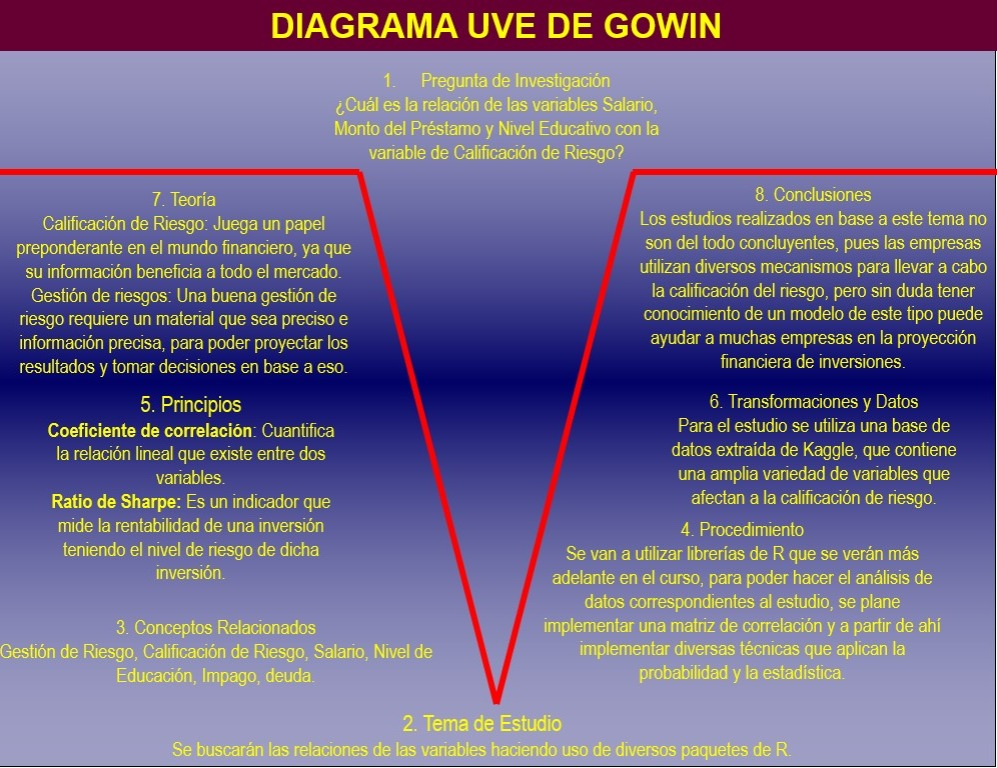
\includegraphics{imagenes/v-gowin.jpeg}

}

\caption{V de Gowin}

\end{figure}%

\subsection{Conceptos básicos}\label{conceptos-buxe1sicos}

Como hemos estado hablando a lo largo del trabajo, la calificación de
riesgo es de suma importancia, por lo que el estudio posee como objetivo
determinar una relación fuerte de las variables, para aproximar un
método empírico de una calificación de riesgo, pues ya vimos que las
empresas por lo general no comparten esta información.

Por otro lado, la gestión de riesgo y la incertidumbre se vuelven
esenciales a lo largo del trabajo, pues son conceptos que son base para
el estudio posterior. El riesgo de impago también se vuelve un concepto
a tener en cuenta, el cual vamos a entender como la incapacidad de
cumplir una obligación financiera.

\subsection{Principios y teorías}\label{principios-y-teoruxedas}

Para llevar a cabo la investigación en estas etapas preliminares hemos
hecho estudio bibliográfico de lo que son los análisis de calificación
financiera, que es justo el tema y variable objetivo de nuestro estudio.
También se incorpora la teoría de la gestión de riesgos, que a su vez
hace uso de técnicas de probabilidad pues dentro de su corpus la idea
principal es maximizar una ganancia en eventos que presentan
incertidumbre, de ahí la estrecha relación que tiene con Probabilidad.

Por otro lado, utilizar los conceptos de la valoración de riesgos
financieros, sirve de base para entender cómo funciona el mercado
financiero, y cuáles son los impactos directos de poseer una
calificación de riesgos, y que el impacto es de hecho, para todos los
participantes.

\section{Parte de escritura}\label{parte-de-escritura}

El problema que se va a tratar en el presente trabajo es de determinar
la relación existente entre las variables de ingresos, nivel de
educación y Monto del préstamo con la calificación de riesgo. Desde el
punto de vista teórico, el autor (Palacios 2012), menciona que ``La
principal función que radica en las calificaciones crediticias es la
evaluación de la mayor o menor probabilidad de pago de la deuda y los
intereses, proporcionando indicadores que sirvan de referencia a los
inversores con el fin de que puedan tener conocimiento del riesgo
crediticio de una forma simple y accesible''. Desde este punto de vista,
hay un apoyo en la investigación que tratamos de realizar, pues la
calificación de riesgo es de suma importancia en el mundo financiero.
Este mismo autor menciona que ``Su importancia deriva de su implantación
dentro de la regulación, lo que afecta a todo el entramado
institucional, y sectores clave de la sociedad como son el bancario y
las agencias de seguros y reaseguros'', podemos ver entonces que la
teoría respalda la importancia que hemos estado conjeturando en esta
presente bitácora (Entiéndase conjeturando, porque aún no hemos
realizado el análisis de la tabla de datos).

El estudio del análisis financiero es de suma importancia en la
actualidad, ya que las transacciones de los flujos de dinero cada vez
son mayores, es decir, vender deuda para obtener financiamiento en el
corto plazo es una de las estrategias más aplicadas, por ello tanto
inversores como prestatarios, según (Palacios 2012), ``Los inversores
hacen uso de las calificaciones crediticias como un indicador de la
probabilidad de recuperar su dinero. Adicionalmente, los prestatarios
pueden beneficiarse de tener calificada su deuda, con el objetivo de
colocarla con mayor facilidad y eliminar las dudas que haya relación a
ellos.'' Por ello, ambas parten obtienen beneficio de que exista este
rating en el mundo de la información financiera. Y desde el punto de
vista del inversor, como menciona la autora (Chicu 2020), ``\ldots a la
hora de analizar una inversión, debemos valorar la rentabilidad
esperada, así como la liquidez que perdemos y el riesgo que estamos
dispuestos a sumir''. Por lo tanto, poseer la información de rating es
de suma utilidad, pues ayuda a los inversores a realizar mejores
proyecciones. En adición, haciendo referencia a esta misma autora
``\ldots la gestión de riesgos tiene un lugar cada vez que un inversor
analiza e intenta cuantificar las pérdidas potenciales en una inversión
y luego toma las medidas apropiadas, considerando sus objetivos de
inversión y su tolerancia al riesgo.'' Esto último viene de la mano con
lo que son las proyecciones, pues le permite al inversionista hacer un
mejor análisis y una gestión de riesgos adecuada, que podemos definir
según Chicu como ``El proceso de identificación, análisis e
incorporación de la incertidumbre en las decisiones de inversión''
(Chicu 2020). Reforzando lo que menciona Chicu, la autora (Maria de los
Ángeles Herrera 2024), menciona en adición a la gestión de riesgos ``el
contexto de incertidumbre genera inevitablemente un riesgo, y es ahí
cuando la institución financiera debe preservar su valor económico y la
integridad de los recursos confiados por los depositantes y socios.'' Y
añadiendo la definición de esta misma autora tenemos que la gestión de
riesgos es ``la denominación que se utiliza para el conjunto de técnicas
y herramientas que pretenden maximizar el valor económico de la
institución financiera, en un contexto de incertidumbre''. Concluyendo,
la gestión de riesgos depende íntimamente de la calificación de riesgo,
pues permite tener un parámetro ante la incertidumbre que representa
invertir.

\bookmarksetup{startatroot}

\chapter{Bitácora 2}\label{bituxe1cora-2}

\section{Parte de Planificación}\label{parte-de-planificaciuxf3n-1}

\subsection{Ordenamiento de la
Literatura}\label{ordenamiento-de-la-literatura}

\textbf{Tabla de Organización y Literatura}

\begin{longtable*}{| p{2.5cm} | p{2cm} | p{2.5cm} | p{3cm} | p{0.8cm} | p{2.5cm} |}
\hline
\textbf{Tipo} & \textbf{Tema General} & \textbf{Tema Específico} & \textbf{Título} & \textbf{Año} & \textbf{Autor(es)} \\
\hline
\fontsize{8pt}{10pt}
Metodológica & Correlación y Análisis de datos & Análisis del perfil de los prestatarios & La evaluación del riesgo de crédito en las instituciones de microfinanzas: estado del arte & 2017 & María Seijas, Milagro Vivel, Rubén Lado, Sara Fernández \\
\hline
Metodológica & Correlación y Análisis de datos & Relevancia del scoring de crédito & Modelos para el otorgamiento y seguimiento en la gestión del riesgo crediticio & 2018 & Millan Solarte, Julio Cesar, Edinson Caicedo \\
\hline
Metodológica & Correlación y Análisis de datos & Relación variables cuantitativas y cualitativas en el incumplimiento de pago & Variables determinantes de la probabilidad de incumplimiento de un microcrédito & 2011 & María Calixto, Luis Casaverde \\
\hline
Metodológica & Correlación y Análisis de datos & Clasificación de perfiles basándose en variables cualitativas & Credit Scoring en Costa Rica y la probabilidad de clasificación de créditos personales & 2013 & Patricia Hernández, José Montoya, Allan Villareal \\
\hline
\end{longtable*}

\normalsize
\newpage

\begin{Shaded}
\begin{Highlighting}[]
\ControlFlowTok{if}\NormalTok{ (}\SpecialCharTok{!}\FunctionTok{requireNamespace}\NormalTok{(}\StringTok{"kableExtra"}\NormalTok{, }\AttributeTok{quietly =} \ConstantTok{TRUE}\NormalTok{)) \{}
  \FunctionTok{install.packages}\NormalTok{(}\StringTok{"kableExtra"}\NormalTok{)}
\NormalTok{\}}
\FunctionTok{library}\NormalTok{(kableExtra)}

\NormalTok{data }\OtherTok{\textless{}{-}} \FunctionTok{data.frame}\NormalTok{(}
  \AttributeTok{Tipo =} \FunctionTok{rep}\NormalTok{(}\StringTok{"Metodológica"}\NormalTok{, }\DecValTok{4}\NormalTok{),}
  \AttributeTok{Tema\_General =} \FunctionTok{rep}\NormalTok{(}\StringTok{"Correlación y Análisis de datos"}\NormalTok{, }\DecValTok{4}\NormalTok{),}
  \AttributeTok{Tema\_Especifico =} \FunctionTok{c}\NormalTok{(}\StringTok{"Análisis del perfil de los prestatarios"}\NormalTok{, }
                      \StringTok{"Relevancia del scoring de crédito"}\NormalTok{, }
                      \StringTok{"Relación variables cuantitativas y cualitativas en el incumplimiento de pago"}\NormalTok{, }
                      \StringTok{"Clasificación de perfiles basándose en variables cualitativas"}\NormalTok{),}
\NormalTok{  Título }\OtherTok{=} \FunctionTok{c}\NormalTok{(}\StringTok{"La evaluación del riesgo de crédito en las instituciones de microfinanzas: estado del arte"}\NormalTok{, }
             \StringTok{"Modelos para el otorgamiento y seguimiento en la gestión del riesgo crediticio"}\NormalTok{, }
             \StringTok{"Variables determinantes de la probabilidad de incumplimiento de un microcrédito"}\NormalTok{, }
             \StringTok{"Credit Scoring en Costa Rica y la probabilidad de clasificación de créditos personales"}\NormalTok{),}
\NormalTok{  Año }\OtherTok{=} \FunctionTok{c}\NormalTok{(}\DecValTok{2017}\NormalTok{, }\DecValTok{2018}\NormalTok{, }\DecValTok{2011}\NormalTok{, }\DecValTok{2013}\NormalTok{),}
  \AttributeTok{Autor =} \FunctionTok{c}\NormalTok{(}\StringTok{"María Seijas, Milagro Vivel, Rubén Lado, Sara Fernández"}\NormalTok{,}
            \StringTok{"Millan Solarte, Julio Cesar, Edinson Caicedo"}\NormalTok{,}
            \StringTok{"María Calixto, Luis Casaverde"}\NormalTok{,}
            \StringTok{"Patricia Hernández, José Montoya, Allan Villareal"}\NormalTok{)}
\NormalTok{)}


\FunctionTok{kable}\NormalTok{(data, }\AttributeTok{format =} \StringTok{"html"}\NormalTok{, }\AttributeTok{escape =} \ConstantTok{FALSE}\NormalTok{, }
      \AttributeTok{col.names =} \FunctionTok{c}\NormalTok{(}\StringTok{"Tipo"}\NormalTok{, }\StringTok{"Tema General"}\NormalTok{, }\StringTok{"Tema Específico"}\NormalTok{, }\StringTok{"Título"}\NormalTok{, }\StringTok{"Año"}\NormalTok{, }\StringTok{"Autor(es)"}\NormalTok{)) }\SpecialCharTok{\%\textgreater{}\%}
  \FunctionTok{kable\_styling}\NormalTok{(}\AttributeTok{full\_width =} \ConstantTok{FALSE}\NormalTok{, }\AttributeTok{position =} \StringTok{"left"}\NormalTok{) }
\end{Highlighting}
\end{Shaded}

\section{Enlaces de la Literatura}\label{enlaces-de-la-literatura}

\textbf{Título:} \emph{La valoración del riesgo financiero}.

\textbf{Resumen:} El riesgo financiero es uno de los tipos de riesgo más
importantes, por eso es de suma importancia entender su significado y
qué herramientas se pueden utilizar para su debida gestión. En este caso
se enfocan en tres métodos distintos: la desviación estándar, la beta
del mercado y el valor en riesgo; así como comprender la rentabilidad
ajustada con el ratio de Sharpe. Al utilizarlos en estrategias de
cobertura de riesgo financiero se logra una reducción o mitigación del
mismo en diferentes intrumentos financieros como las carteras de
inversión.

\textbf{Contraste:} Este trabajo, a comparación del artículo de Solarte
J. y Caicedo E. titulado Modelos para otorgamiento y seguimiento en la
gestión del riesgo de crédito, logra explicar de manera más amigable y
general los conceptos del riesgo financiero, lo que hace que el artículo
de Chicu sea más comprensible para todas las personas. Sin embargo, esta
falta de rigurosidad puede generar fallas en los procesos más complejos
del tema de investigación, ya que el mismo artículo de Solarte y Caicedo
utiliza fórmulas y métodos más complejos que si bien no son tan fáciles
de entender, logran una mejor recopilación de resultados.

\textbf{Comentario Propio:} Si bien nos parece importante que una
explicación sea comprensible para la mayor cantidad de personas, no
tener la suficiente precisión en un tema tan complicado como lo es el
riesgo financiero puede causar ignorancia en los conceptos avanzados,
como por ejemplo los métodos paramétricos y no paramétricos y su
metodología. Sin embargo, sentimos que esta investigación nos ayudó con
la afinidad a la hora de seleccionar las palabras adecuadas en el
desarrollo de nuestra investigación.

\textbf{Título:} \emph{La evaluación del riesgo de crédito en las
instituciones de microfinanzas: estado del arte}.

\textbf{Resumen:} El análisis de los modelos de credit scoring muestra
que estos pueden ser utilizados en diversas dimensiones, aunque hay una
preferencia por predecir el riesgo de retrasos costosos en los
microcréditos los cuales están bajo control de las instituciones
financieras para mitigarlos. La literatura teórica destaca la
importancia de la información estadística cualitativa en estos modelos,
además de incluir variables relacionadas con el prestatario, su negocio
y el préstamo. Existe una preferencia por las téncicas paramétricas como
por ejemplo la regresión logística. Aún así, en los últimos años se
registra un aumento en el uso de técnicas no paramétricas que logran un
mayor poder predictivo en la detección de incumplimientos de
microcréditos. Con esto, las instituciones están incorporando estas
herramientas para convertirlas en una práctica estándar, como en las
instituciones bancarias; las cuales mejoran la consistencia,
transparencia, control de calidad y optimización de los procesos.

\textbf{Contraste:} Éste trabajo, a diferencia del artículo de Chicu D.
titulado La valoración del riesgo financiero, logra realizar no sólo un
análisis del credit scoring por medio de teoría estadística, sino que
también logra plantear un análisis macroeconómico y toma en cuenta las
repercusiones que las fallas en los procesos de gestion de riesgos
podría generar en el sistema financiero. Sin embargo, no es tan
específico en la parte matemática a la hora de estimar probabilidades de
que algo pase.

\textbf{Comentario Propio:} Para nosotros es importante entender también
la teoría desde la perspectiva economista ya que nos ayuda a entender a
qué nos enfrentamos y cómo podemos aplicar diferentes metodologías de
investigación.

\textbf{Título:} \emph{Modelos para otorgamiento y seguimiento en la
gestión del riesgo de crédito.}

\textbf{Resumen:} El credit scoring es un método estadístico para
estimar la probabilidad de inclumpimiento de un prestatario, usando su
información histórica y estadística para obtener un indicador que
permita distinguir la calidad de un deudor. Los modelos de scoring son
muy importantes para los procesos de gestión del crédito, los cuales
buscan explicar la composición y operatividad de estos modelos
utilizando grandes bases de datos. La información que resulta de estos
modelos permite el análisis de la toma de decisión de si se otorga ó no
un crédito a una persona. Por medio de cuatro modelos distintos se logra
un procedimiento multicapa para obtener información precisa para
calificar a un cliente como bueno o malo para la empresa financiera.

\textbf{Contraste:} Este trabajo logra ser más específico que los demás
en cuanto a los métodos de gestión de riesgo se refiere. Además coincide
con varios de los artículos recopilados respecto a la utilización del
método de regresión logística como herramienta de calificación de
crédito.

\textbf{Comentario Propio:} Consideramos que este artículo es el más
completo en cuanto a materia matemática se refiere, ya que logra
explicar los métodos de manera clara y además los muestra con las
gráficas y resultados obtenidos. De hecho, es de gran ayuda que las
variables a trabajar sean similares a las que la investigación utiliza.

\textbf{Título:} \emph{Variables determinantes de la probabilidad de
incumplimiento de un microcrédito en una entidad microfinanciera del
Perú, una aproximación bajo el modelo de regresión logística binaria.}

\textbf{Resumen:} Después de realizar una estimación probabilística del
incumplimiento de un microcrédito por medio de la aproximación de una
función logística binaria, se determina que son las variables
cualitativas como el estado civil, edad y tipo de vivienda junto con las
variables de plazo, número de créditos con la entidad y el saldo deudor;
las que generan un modelo correctamente ajustado bajo el modelo de
regresión logística. La cual logra una capacidad predictiva aceptable
medida por la curva ROC.

\textbf{Contraste:} Este trabajo, a diferencia de ``La evaluación del
riesgo de crédito en las instituciones de microfinanzas: estado del
arte'', determina las variables necesarias para un estudio de
microfinanzas. Sin embargo, coinciden en todo lo referente a las
ventajas y deventajas del uso de la calificación crediticia, aunque si
cabe mencionar que esta investigación tambien logra hacer conclusiones
de los inversores y reguladores como parte de los responsables de la
ineficiencia que ha dado el uso excesivo de ésta calificación.

\textbf{Comentario Propio:} Fue de mucha ayuda entender la noción de qué
variables utilizar y porqué son importantes para un estudio de
calificación de crédito.

\textbf{Título:} \emph{Calificación de riesgo: definición e influencia
en la última década}.

\textbf{Resumen:} Las agencias de calificación crediticia han crecido en
las últimas décadas por su capacidad para reducir las asimetrías de
información en los mercados, facilitando la liquidez y aumentando los
participantes. Sin embargo, no han cumplido con los efectos positivos
esperados en la última década, se han expuesto fallas en su
funcionamiento, como su papel en la burbuja de deuda y la crisis
económica, lo que ha generado inestabilidad y ralentizado la
recuperación. La importancia que los inversores le dieron a las
calificaciones crediticias para la toma de desiciones fue desmedida al
no tomar en cuenta el nivel de riesgo, lo cual se relaciona a las causas
de las últimas crisis financieras e hipotecarias.

\textbf{Contraste:} En comparación de la investigación titulada ``La
evaluación del riesgo de crédito en las instituciones de microfinanzas:
estado del arte'', ambos logran concluir cosas muy similares en cuanto a
la importancia del credit score, sus ventajas y desventajas. Sin
embargo, logra aportar más en cuanto a las ineficiencias que ha tenido
sobrevalorarlo y los momentos en los que ha generado una crisis.

\textbf{Comentario Propio:} Este trabajo, de igual forma, es de suma
importancia para entender la manera en que se realizan calificaciones
crediticias y de qué formas analizarlas. Para así utilizarlas en
nuestros estudios estadísticos y entender qué otras variables ó
conceptos tomar en cuenta para los futuros resultados a obtener.

\textbf{Título:} Conceptualización del riesgo de los mercados
financieros.

\textbf{Resumen:} El riesgo está inmerso en todas las actividades
humanas y es entendido como la probabilidad de ocurrencia de un evento
que podría inducir un perjuicio. Cuando se habla de riesgo financiero,
se habla de una eventual pérdida de dinero que signifique una afectación
al sistema financiero ó a alguna institución que sea parte del mismo.
Este trabajo es una recopilación algunos de los riesgos en los mercados
financieros y presenta algunos métodos válidos para su valoración.

\textbf{Contraste:} Esta investigación, a diferencia de las demás
investigaciones, logra tener un glosario completo de definiciones
relacionadas al riesgo financiero, sin embargo no va más allá de ser
sólamente un artículo de definiciones. Por lo que en materia teórica no
tiene nada que aportar.

\textbf{Comentario Propio:} Gracias a estas definiciones, hemos logrado
definir mejor qué queremos estudiar de manera más específica y cómo
utilizar ciertos conceptos de mejor manera.

\section{Análisis Estadístico}\label{anuxe1lisis-estaduxedstico}

Como base para realizar este análisis estadístico, nos estamos guíando
con la guía del curso de Herramientas de Ciencias de Datos, el cual
adjuntamos el link a dicha guía (Solis 2024) y también estamos
utilizando el libro escrito por Wickham, el cual también adjuntamos el
link (Hadley Wickham 2019).

A modo de introducción, el análisis estadístico consiste en un conjunto
de herramientas o técnias que se utilizan para la recolección, el
análisis e interpretación de datos. Para este trabajo es imprescindible
contar con este set de herramientas.

\subsection{Análisis Descriptivo}\label{anuxe1lisis-descriptivo}

La base de datos ya se encuentra en formato en tidy, recordemos que el
formato tidy fue popularizado por el autor Hadley Wickham, donde indican
que cada variable debe tener su propia columna y cada observación su
propia fila. Nuestra base de datos cumple con estar en formato tidy.

Vamos a llamar a nuestra base de datos, la cual vamos a utilizar durante
el trabajo.

\begin{verbatim}
Rows: 15000 Columns: 20
-- Column specification --------------------------------------------------------
Delimiter: ";"
chr (10): Gender, Education Level, Marital Status, Loan Purpose, Employment ...
dbl (10): Age, Income, Credit Score, Loan Amount, Years at Current Job, Debt...

i Use `spec()` to retrieve the full column specification for this data.
i Specify the column types or set `show_col_types = FALSE` to quiet this message.
\end{verbatim}

\begin{Shaded}
\begin{Highlighting}[]
\FunctionTok{head}\NormalTok{(base\_financial\_risk\_assessment)}
\end{Highlighting}
\end{Shaded}

\begin{verbatim}
# A tibble: 6 x 20
    Age Gender     `Education Level` `Marital Status` Income `Credit Score`
  <dbl> <chr>      <chr>             <chr>             <dbl>          <dbl>
1    49 Male       PhD               Divorced          72799            688
2    57 Female     Bachelor's        Widowed              NA            690
3    21 Non-binary Master's          Single            55687            600
4    59 Male       Bachelor's        Single            26508            622
5    25 Non-binary Bachelor's        Widowed           49427            766
6    30 Non-binary PhD               Divorced             NA            717
# i 14 more variables: `Loan Amount` <dbl>, `Loan Purpose` <chr>,
#   `Employment Status` <chr>, `Years at Current Job` <dbl>,
#   `Payment History` <chr>, `Debt-to-Income Ratio` <dbl>,
#   `Assets Value` <dbl>, `Number of Dependents` <dbl>, City <chr>,
#   State <chr>, Country <chr>, `Previous Defaults` <dbl>,
#   `Marital Status Change` <dbl>, `Risk Rating` <chr>
\end{verbatim}

Antes de aplicar cualquier gráfico o análisis de datos a nuestra base de
datos, es importante eliminar las variables que no aportan al estudio,
por ello, vamos a eliminar los valores NA que vengan en nuestra base de
datos.

\begin{Shaded}
\begin{Highlighting}[]
\NormalTok{Base\_limpia }\OtherTok{\textless{}{-}} \FunctionTok{na.omit}\NormalTok{(base\_financial\_risk\_assessment)}
\FunctionTok{head}\NormalTok{(Base\_limpia)}
\end{Highlighting}
\end{Shaded}

\begin{verbatim}
# A tibble: 6 x 20
    Age Gender     `Education Level` `Marital Status` Income `Credit Score`
  <dbl> <chr>      <chr>             <chr>             <dbl>          <dbl>
1    49 Male       PhD               Divorced          72799            688
2    21 Non-binary Master's          Single            55687            600
3    59 Male       Bachelor's        Single            26508            622
4    42 Non-binary Master's          Single           116212            707
5    55 Male       High School       Married           70978            706
6    56 Non-binary PhD               Married           21084            702
# i 14 more variables: `Loan Amount` <dbl>, `Loan Purpose` <chr>,
#   `Employment Status` <chr>, `Years at Current Job` <dbl>,
#   `Payment History` <chr>, `Debt-to-Income Ratio` <dbl>,
#   `Assets Value` <dbl>, `Number of Dependents` <dbl>, City <chr>,
#   State <chr>, Country <chr>, `Previous Defaults` <dbl>,
#   `Marital Status Change` <dbl>, `Risk Rating` <chr>
\end{verbatim}

Ahora hacemos un análisis estadístico de nuestra base de datos, de todas
las variables.

\begin{Shaded}
\begin{Highlighting}[]
\CommentTok{\# Instalar kableExtra si no lo tienes}
\CommentTok{\# install.packages("kableExtra") }

\FunctionTok{library}\NormalTok{(dplyr)}
\FunctionTok{library}\NormalTok{(tidyr)}
\FunctionTok{library}\NormalTok{(knitr)}
\FunctionTok{library}\NormalTok{(kableExtra)}

\CommentTok{\# Como nuestras variables no son del todo numéricas, hay que hacerlo para las variables que son numéricas y para las variables que son categóricas. }

\CommentTok{\# Primero hacemos las variables numéricas.}
\NormalTok{resumen\_numericas }\OtherTok{\textless{}{-}}\NormalTok{ Base\_limpia }\SpecialCharTok{\%\textgreater{}\%}
  \FunctionTok{summarise}\NormalTok{(}
    \AttributeTok{Edad\_Media =} \FunctionTok{mean}\NormalTok{(Age, }\AttributeTok{na.rm =} \ConstantTok{TRUE}\NormalTok{),}
    \AttributeTok{Edad\_Minima =} \FunctionTok{min}\NormalTok{(Age, }\AttributeTok{na.rm =} \ConstantTok{TRUE}\NormalTok{),}
    \AttributeTok{Edad\_Maxima =} \FunctionTok{max}\NormalTok{(Age, }\AttributeTok{na.rm =} \ConstantTok{TRUE}\NormalTok{),}
    \AttributeTok{Ingreso\_Medio =} \FunctionTok{mean}\NormalTok{(Income, }\AttributeTok{na.rm =} \ConstantTok{TRUE}\NormalTok{),}
    \AttributeTok{Ingreso\_Varianza =} \FunctionTok{var}\NormalTok{(Income, }\AttributeTok{na.rm =} \ConstantTok{TRUE}\NormalTok{),}
    \AttributeTok{Ingreso\_Minimo =} \FunctionTok{min}\NormalTok{(Income, }\AttributeTok{na.rm =} \ConstantTok{TRUE}\NormalTok{),}
    \AttributeTok{Ingreso\_Maximo =} \FunctionTok{max}\NormalTok{(Income, }\AttributeTok{na.rm =} \ConstantTok{TRUE}\NormalTok{),}
    \AttributeTok{Prestamo\_Medio =} \FunctionTok{mean}\NormalTok{(}\StringTok{\textasciigrave{}}\AttributeTok{Loan Amount}\StringTok{\textasciigrave{}}\NormalTok{, }\AttributeTok{na.rm =} \ConstantTok{TRUE}\NormalTok{),}
    \AttributeTok{Prestamo\_Varianza =} \FunctionTok{var}\NormalTok{(}\StringTok{\textasciigrave{}}\AttributeTok{Loan Amount}\StringTok{\textasciigrave{}}\NormalTok{, }\AttributeTok{na.rm =} \ConstantTok{TRUE}\NormalTok{),}
    \AttributeTok{Prestamo\_Minimo =} \FunctionTok{min}\NormalTok{(}\StringTok{\textasciigrave{}}\AttributeTok{Loan Amount}\StringTok{\textasciigrave{}}\NormalTok{, }\AttributeTok{na.rm =} \ConstantTok{TRUE}\NormalTok{),}
    \AttributeTok{Prestamo\_Maximo =} \FunctionTok{max}\NormalTok{(}\StringTok{\textasciigrave{}}\AttributeTok{Loan Amount}\StringTok{\textasciigrave{}}\NormalTok{, }\AttributeTok{na.rm =} \ConstantTok{TRUE}\NormalTok{)}
\NormalTok{  )}

\CommentTok{\# Variables Categóricas}
\NormalTok{resumen\_categoricas }\OtherTok{\textless{}{-}} \FunctionTok{tibble}\NormalTok{(}
  \AttributeTok{Variable =} \FunctionTok{c}\NormalTok{(}\StringTok{"Nivel de Educación"}\NormalTok{, }\StringTok{"Género"}\NormalTok{, }\StringTok{"Estado Civil"}\NormalTok{),}
  \AttributeTok{Frecuencia =} \FunctionTok{c}\NormalTok{(}
    \FunctionTok{paste}\NormalTok{(}\FunctionTok{names}\NormalTok{(}\FunctionTok{table}\NormalTok{(Base\_limpia}\SpecialCharTok{$}\StringTok{\textasciigrave{}}\AttributeTok{Education Level}\StringTok{\textasciigrave{}}\NormalTok{)), }\AttributeTok{collapse =} \StringTok{", "}\NormalTok{),}
    \FunctionTok{paste}\NormalTok{(}\FunctionTok{names}\NormalTok{(}\FunctionTok{table}\NormalTok{(Base\_limpia}\SpecialCharTok{$}\NormalTok{Gender)), }\AttributeTok{collapse =} \StringTok{", "}\NormalTok{),}
    \FunctionTok{paste}\NormalTok{(}\FunctionTok{names}\NormalTok{(}\FunctionTok{table}\NormalTok{(Base\_limpia}\SpecialCharTok{$}\StringTok{\textasciigrave{}}\AttributeTok{Marital Status}\StringTok{\textasciigrave{}}\NormalTok{)), }\AttributeTok{collapse =} \StringTok{", "}\NormalTok{)}
\NormalTok{  )}
\NormalTok{)}

\CommentTok{\# Luego resumimos la información en un cuadro, para presentarlo mejor.}
\NormalTok{tabla\_resumen }\OtherTok{\textless{}{-}} \FunctionTok{data.frame}\NormalTok{(}
  \AttributeTok{Variable =} \FunctionTok{c}\NormalTok{(}\StringTok{"Edad"}\NormalTok{, }\StringTok{"Ingresos"}\NormalTok{, }\StringTok{"Monto del Préstamo"}\NormalTok{, resumen\_categoricas}\SpecialCharTok{$}\NormalTok{Variable),}
  \AttributeTok{Media =} \FunctionTok{c}\NormalTok{(resumen\_numericas}\SpecialCharTok{$}\NormalTok{Edad\_Media, resumen\_numericas}\SpecialCharTok{$}\NormalTok{Ingreso\_Medio, resumen\_numericas}\SpecialCharTok{$}\NormalTok{Prestamo\_Medio, }\FunctionTok{rep}\NormalTok{(}\ConstantTok{NA}\NormalTok{, }\DecValTok{3}\NormalTok{)),}
  \AttributeTok{Varianza =} \FunctionTok{c}\NormalTok{(}\ConstantTok{NA}\NormalTok{, resumen\_numericas}\SpecialCharTok{$}\NormalTok{Ingreso\_Varianza, resumen\_numericas}\SpecialCharTok{$}\NormalTok{Prestamo\_Varianza, }\FunctionTok{rep}\NormalTok{(}\ConstantTok{NA}\NormalTok{, }\DecValTok{3}\NormalTok{)),}
\NormalTok{  Mínimo }\OtherTok{=} \FunctionTok{c}\NormalTok{(resumen\_numericas}\SpecialCharTok{$}\NormalTok{Edad\_Minima, resumen\_numericas}\SpecialCharTok{$}\NormalTok{Ingreso\_Minimo, resumen\_numericas}\SpecialCharTok{$}\NormalTok{Prestamo\_Minimo, }\FunctionTok{rep}\NormalTok{(}\ConstantTok{NA}\NormalTok{, }\DecValTok{3}\NormalTok{)),}
\NormalTok{  Máximo }\OtherTok{=} \FunctionTok{c}\NormalTok{(resumen\_numericas}\SpecialCharTok{$}\NormalTok{Edad\_Maxima, resumen\_numericas}\SpecialCharTok{$}\NormalTok{Ingreso\_Maximo, resumen\_numericas}\SpecialCharTok{$}\NormalTok{Prestamo\_Maximo, }\FunctionTok{rep}\NormalTok{(}\ConstantTok{NA}\NormalTok{, }\DecValTok{3}\NormalTok{)),}
  \AttributeTok{Frecuencia =} \FunctionTok{c}\NormalTok{(}\FunctionTok{rep}\NormalTok{(}\ConstantTok{NA}\NormalTok{, }\DecValTok{3}\NormalTok{), resumen\_categoricas}\SpecialCharTok{$}\NormalTok{Frecuencia)}
\NormalTok{)}

\CommentTok{\# Mostrar la tabla con la descripción}
\NormalTok{tabla\_resumen\_kable }\OtherTok{\textless{}{-}} \FunctionTok{kable}\NormalTok{(tabla\_resumen, }\AttributeTok{caption =} \StringTok{"Resumen de Variables Numéricas y Categóricas"}\NormalTok{) }\SpecialCharTok{\%\textgreater{}\%}
  \FunctionTok{kable\_styling}\NormalTok{() }\SpecialCharTok{\%\textgreater{}\%}
  \FunctionTok{add\_header\_above}\NormalTok{(}\FunctionTok{c}\NormalTok{(}\StringTok{" "} \OtherTok{=} \DecValTok{1}\NormalTok{, }\StringTok{"Resumen"} \OtherTok{=} \DecValTok{5}\NormalTok{)) }
\NormalTok{tabla\_resumen\_kable }\OtherTok{\textless{}{-}}\NormalTok{ tabla\_resumen\_kable }\SpecialCharTok{\%\textgreater{}\%}
\NormalTok{  kableExtra}\SpecialCharTok{::}\FunctionTok{footnote}\NormalTok{(}\AttributeTok{general =} \StringTok{"Fuente: Elaboración propia utilizando la base de datos de Kaggle"}\NormalTok{)}
\NormalTok{tabla\_resumen\_kable}
\end{Highlighting}
\end{Shaded}

\begin{longtable}[t]{lrrrrl}
\caption{Resumen de Variables Numéricas y Categóricas}\\
\toprule
\multicolumn{1}{c}{ } & \multicolumn{5}{c}{Resumen} \\
\cmidrule(l{3pt}r{3pt}){2-6}
Variable & Media & Varianza & Mínimo & Máximo & Frecuencia\\
\midrule
Edad & 43.5817 & NA & 18 & 69 & NA\\
Ingresos & 70190.3585 & 849685113 & 20014 & 119978 & NA\\
Monto del Préstamo & 27577.0679 & 168240584 & 5001 & 49978 & NA\\
Nivel de Educación & NA & NA & NA & NA & Bachelor's, High School, Master's, PhD\\
Género & NA & NA & NA & NA & Female, Male, Non-binary\\
\addlinespace
Estado Civil & NA & NA & NA & NA & Divorced, Married, Single, Widowed\\
\bottomrule
\multicolumn{6}{l}{\rule{0pt}{1em}\textit{Note: }}\\
\multicolumn{6}{l}{\rule{0pt}{1em}Fuente: Elaboración propia utilizando la base de datos de Kaggle}\\
\end{longtable}

Presentamos las variables de más importancia en nuestro estudio

\begin{longtable}[t]{lrrrrl}
\caption{Resumen de Variables Numéricas y Categóricas}\\
\toprule
\multicolumn{1}{c}{ } & \multicolumn{5}{c}{Resumen} \\
\cmidrule(l{3pt}r{3pt}){2-6}
Variable & Media & Varianza & Mínimo & Máximo & Frecuencia\\
\midrule
Edad & 43.5817 & NA & 18 & 69 & NA\\
Ingresos & 70190.3585 & 849685113 & 20014 & 119978 & NA\\
Monto del Préstamo & 27577.0679 & 168240584 & 5001 & 49978 & NA\\
Nivel de Educación & NA & NA & NA & NA & Bachelor's, High School, Master's, PhD\\
Género & NA & NA & NA & NA & Female, Male, Non-binary\\
\addlinespace
Estado Civil & NA & NA & NA & NA & Divorced, Married, Single, Widowed\\
\bottomrule
\multicolumn{6}{l}{\rule{0pt}{1em}\textit{Note: }}\\
\multicolumn{6}{l}{\rule{0pt}{1em}Fuente: Elaboración propia utilizando la base de datos de Kaggle}\\
\end{longtable}

Con nuestra base de datos limpia, vanmos a proceder a calcular algunos
estadísticos importantes, por separado. Estos son los datos resumidos de
la variable edad.

\begin{Shaded}
\begin{Highlighting}[]
\FunctionTok{library}\NormalTok{(dplyr)}

\CommentTok{\# Calculamos las estadísticas de interés para las variables y las almacenamos en un solo data.frame}
\NormalTok{resultado }\OtherTok{\textless{}{-}}\NormalTok{ Base\_limpia }\SpecialCharTok{\%\textgreater{}\%} 
  \FunctionTok{summarise}\NormalTok{(}
    \CommentTok{\# Estadísticos para la variable edad/Age}
    \AttributeTok{media\_edad =} \FunctionTok{mean}\NormalTok{(Age, }\AttributeTok{na.rm =} \ConstantTok{TRUE}\NormalTok{),}
    \AttributeTok{varianza\_edad =} \FunctionTok{var}\NormalTok{(Age, }\AttributeTok{na.rm =} \ConstantTok{TRUE}\NormalTok{),}
    \AttributeTok{min\_edad =} \FunctionTok{min}\NormalTok{(Age, }\AttributeTok{na.rm =} \ConstantTok{TRUE}\NormalTok{),}
    \AttributeTok{max\_edad =} \FunctionTok{max}\NormalTok{(Age, }\AttributeTok{na.rm =} \ConstantTok{TRUE}\NormalTok{),}
    
    \CommentTok{\# Estadísticos para la variable ingreso/Income}
    \AttributeTok{media\_ingresos =} \FunctionTok{mean}\NormalTok{(Income, }\AttributeTok{na.rm =} \ConstantTok{TRUE}\NormalTok{),}
    \AttributeTok{varianza\_ingresos =} \FunctionTok{var}\NormalTok{(Income, }\AttributeTok{na.rm =} \ConstantTok{TRUE}\NormalTok{),}
    \AttributeTok{min\_ingresos =} \FunctionTok{min}\NormalTok{(Income, }\AttributeTok{na.rm =} \ConstantTok{TRUE}\NormalTok{),}
    \AttributeTok{max\_ingresos =} \FunctionTok{max}\NormalTok{(Income, }\AttributeTok{na.rm =} \ConstantTok{TRUE}\NormalTok{),}
    
    \CommentTok{\# Estadísticos para la variable record\_crediticio/Credit Score}
    \AttributeTok{media\_record\_crediticio =} \FunctionTok{mean}\NormalTok{(}\StringTok{\textasciigrave{}}\AttributeTok{Credit Score}\StringTok{\textasciigrave{}}\NormalTok{, }\AttributeTok{na.rm =} \ConstantTok{TRUE}\NormalTok{),}
    \AttributeTok{varianza\_record\_crediticio =} \FunctionTok{var}\NormalTok{(}\StringTok{\textasciigrave{}}\AttributeTok{Credit Score}\StringTok{\textasciigrave{}}\NormalTok{, }\AttributeTok{na.rm =} \ConstantTok{TRUE}\NormalTok{),}
    \AttributeTok{min\_record\_crediticio =} \FunctionTok{min}\NormalTok{(}\StringTok{\textasciigrave{}}\AttributeTok{Credit Score}\StringTok{\textasciigrave{}}\NormalTok{, }\AttributeTok{na.rm =} \ConstantTok{TRUE}\NormalTok{),}
    \AttributeTok{max\_record\_crediticio =} \FunctionTok{max}\NormalTok{(}\StringTok{\textasciigrave{}}\AttributeTok{Credit Score}\StringTok{\textasciigrave{}}\NormalTok{, }\AttributeTok{na.rm =} \ConstantTok{TRUE}\NormalTok{),}
    
    \CommentTok{\# Estadísticos para la variable monto del préstamo/Loan Amount}
    \AttributeTok{media\_monto\_prestamo =} \FunctionTok{mean}\NormalTok{(}\StringTok{\textasciigrave{}}\AttributeTok{Loan Amount}\StringTok{\textasciigrave{}}\NormalTok{, }\AttributeTok{na.rm =} \ConstantTok{TRUE}\NormalTok{),}
    \AttributeTok{varianza\_monto\_prestamo =} \FunctionTok{var}\NormalTok{(}\StringTok{\textasciigrave{}}\AttributeTok{Loan Amount}\StringTok{\textasciigrave{}}\NormalTok{, }\AttributeTok{na.rm =} \ConstantTok{TRUE}\NormalTok{),}
    \AttributeTok{min\_monto\_prestamo =} \FunctionTok{min}\NormalTok{(}\StringTok{\textasciigrave{}}\AttributeTok{Loan Amount}\StringTok{\textasciigrave{}}\NormalTok{, }\AttributeTok{na.rm =} \ConstantTok{TRUE}\NormalTok{),}
    \AttributeTok{max\_monto\_prestamo =} \FunctionTok{max}\NormalTok{(}\StringTok{\textasciigrave{}}\AttributeTok{Loan Amount}\StringTok{\textasciigrave{}}\NormalTok{, }\AttributeTok{na.rm =} \ConstantTok{TRUE}\NormalTok{),}
    
    \CommentTok{\# Estadísticos para la variable años de trabajo/Years at Current Job}
    \AttributeTok{media\_anyos\_trabajo =} \FunctionTok{mean}\NormalTok{(}\StringTok{\textasciigrave{}}\AttributeTok{Years at Current Job}\StringTok{\textasciigrave{}}\NormalTok{, }\AttributeTok{na.rm =} \ConstantTok{TRUE}\NormalTok{),}
    \AttributeTok{varianza\_anyos\_trabajo =} \FunctionTok{var}\NormalTok{(}\StringTok{\textasciigrave{}}\AttributeTok{Years at Current Job}\StringTok{\textasciigrave{}}\NormalTok{, }\AttributeTok{na.rm =} \ConstantTok{TRUE}\NormalTok{),}
    \AttributeTok{min\_anyos\_trabajo =} \FunctionTok{min}\NormalTok{(}\StringTok{\textasciigrave{}}\AttributeTok{Years at Current Job}\StringTok{\textasciigrave{}}\NormalTok{, }\AttributeTok{na.rm =} \ConstantTok{TRUE}\NormalTok{),}
    \AttributeTok{max\_anyos\_trabajo =} \FunctionTok{max}\NormalTok{(}\StringTok{\textasciigrave{}}\AttributeTok{Years at Current Job}\StringTok{\textasciigrave{}}\NormalTok{, }\AttributeTok{na.rm =} \ConstantTok{TRUE}\NormalTok{)}
\NormalTok{  )}

\CommentTok{\# Imprimimos el resultado}
\FunctionTok{print}\NormalTok{(resultado)}
\end{Highlighting}
\end{Shaded}

\begin{verbatim}
# A tibble: 1 x 20
  media_edad varianza_edad min_edad max_edad media_ingresos varianza_ingresos
       <dbl>         <dbl>    <dbl>    <dbl>          <dbl>             <dbl>
1       43.6          218.       18       69         70190.        849685113.
# i 14 more variables: min_ingresos <dbl>, max_ingresos <dbl>,
#   media_record_crediticio <dbl>, varianza_record_crediticio <dbl>,
#   min_record_crediticio <dbl>, max_record_crediticio <dbl>,
#   media_monto_prestamo <dbl>, varianza_monto_prestamo <dbl>,
#   min_monto_prestamo <dbl>, max_monto_prestamo <dbl>,
#   media_anyos_trabajo <dbl>, varianza_anyos_trabajo <dbl>,
#   min_anyos_trabajo <dbl>, max_anyos_trabajo <dbl>
\end{verbatim}

\begin{Shaded}
\begin{Highlighting}[]
\NormalTok{resultado}\SpecialCharTok{$}\NormalTok{media\_edad}
\end{Highlighting}
\end{Shaded}

\begin{verbatim}
[1] 43.5817
\end{verbatim}

\begin{Shaded}
\begin{Highlighting}[]
\NormalTok{resultado}\SpecialCharTok{$}\NormalTok{varianza\_edad}
\end{Highlighting}
\end{Shaded}

\begin{verbatim}
[1] 217.7303
\end{verbatim}

\begin{Shaded}
\begin{Highlighting}[]
\NormalTok{resultado}\SpecialCharTok{$}\NormalTok{min\_edad}
\end{Highlighting}
\end{Shaded}

\begin{verbatim}
[1] 18
\end{verbatim}

\begin{Shaded}
\begin{Highlighting}[]
\NormalTok{resultado}\SpecialCharTok{$}\NormalTok{max\_edad}
\end{Highlighting}
\end{Shaded}

\begin{verbatim}
[1] 69
\end{verbatim}

Estos son los datos resumidos de la variable Ingresos

\begin{Shaded}
\begin{Highlighting}[]
\NormalTok{resultado}\SpecialCharTok{$}\NormalTok{media\_ingresos}
\end{Highlighting}
\end{Shaded}

\begin{verbatim}
[1] 70190.36
\end{verbatim}

\begin{Shaded}
\begin{Highlighting}[]
\NormalTok{resultado}\SpecialCharTok{$}\NormalTok{varianza\_ingresos}
\end{Highlighting}
\end{Shaded}

\begin{verbatim}
[1] 849685113
\end{verbatim}

\begin{Shaded}
\begin{Highlighting}[]
\NormalTok{resultado}\SpecialCharTok{$}\NormalTok{min\_ingresos}
\end{Highlighting}
\end{Shaded}

\begin{verbatim}
[1] 20014
\end{verbatim}

\begin{Shaded}
\begin{Highlighting}[]
\NormalTok{resultado}\SpecialCharTok{$}\NormalTok{max\_ingresos}
\end{Highlighting}
\end{Shaded}

\begin{verbatim}
[1] 119978
\end{verbatim}

Estos son los datos resumidos de la variable Monto del Préstamo

\begin{Shaded}
\begin{Highlighting}[]
\NormalTok{resultado}\SpecialCharTok{$}\NormalTok{media\_monto\_prestamo}
\end{Highlighting}
\end{Shaded}

\begin{verbatim}
[1] 27577.07
\end{verbatim}

\begin{Shaded}
\begin{Highlighting}[]
\NormalTok{resultado}\SpecialCharTok{$}\NormalTok{varianza\_monto\_prestamo}
\end{Highlighting}
\end{Shaded}

\begin{verbatim}
[1] 168240584
\end{verbatim}

\begin{Shaded}
\begin{Highlighting}[]
\NormalTok{resultado}\SpecialCharTok{$}\NormalTok{min\_monto\_prestamo}
\end{Highlighting}
\end{Shaded}

\begin{verbatim}
[1] 5001
\end{verbatim}

\begin{Shaded}
\begin{Highlighting}[]
\NormalTok{resultado}\SpecialCharTok{$}\NormalTok{max\_monto\_prestamo}
\end{Highlighting}
\end{Shaded}

\begin{verbatim}
[1] 49978
\end{verbatim}

Resumimos la información obtenida en un cuadro, para una mejor
visualización de ellos.

\begin{Shaded}
\begin{Highlighting}[]
\FunctionTok{library}\NormalTok{(knitr)}
\FunctionTok{library}\NormalTok{(kableExtra)}

\CommentTok{\# Creamos una tabla para resumir la información obtenida}
\NormalTok{tabla\_resumen }\OtherTok{\textless{}{-}} \FunctionTok{data.frame}\NormalTok{(}
  \AttributeTok{Variable =} \FunctionTok{c}\NormalTok{(}\StringTok{"Edad"}\NormalTok{, }\StringTok{"Ingresos"}\NormalTok{, }\StringTok{"Monto del Préstamo"}\NormalTok{),}
  \AttributeTok{Media =} \FunctionTok{c}\NormalTok{(resultado}\SpecialCharTok{$}\NormalTok{media\_edad, resultado}\SpecialCharTok{$}\NormalTok{media\_ingresos, resultado}\SpecialCharTok{$}\NormalTok{media\_monto\_prestamo),}
  \AttributeTok{Varianza =} \FunctionTok{c}\NormalTok{(}\ConstantTok{NA}\NormalTok{, resultado}\SpecialCharTok{$}\NormalTok{varianza\_ingresos, resultado}\SpecialCharTok{$}\NormalTok{varianza\_monto\_prestamo),}
\NormalTok{  Mínimo }\OtherTok{=} \FunctionTok{c}\NormalTok{(resultado}\SpecialCharTok{$}\NormalTok{min\_edad, resultado}\SpecialCharTok{$}\NormalTok{min\_ingresos, resultado}\SpecialCharTok{$}\NormalTok{min\_monto\_prestamo),}
\NormalTok{  Máximo }\OtherTok{=} \FunctionTok{c}\NormalTok{(resultado}\SpecialCharTok{$}\NormalTok{max\_edad, resultado}\SpecialCharTok{$}\NormalTok{max\_ingresos, resultado}\SpecialCharTok{$}\NormalTok{max\_monto\_prestamo)}
\NormalTok{)}

\CommentTok{\# Mostramos la tabla con la descripción}
\NormalTok{tabla\_resumen\_kable }\OtherTok{\textless{}{-}} \FunctionTok{kable}\NormalTok{(tabla\_resumen, }\AttributeTok{caption =} \StringTok{"Resumen de Variables: Edad, Ingresos y Monto del Préstamo"}\NormalTok{) }\SpecialCharTok{\%\textgreater{}\%}
  \FunctionTok{kable\_styling}\NormalTok{()}

\NormalTok{tabla\_resumen\_kable }\OtherTok{\textless{}{-}}\NormalTok{ tabla\_resumen\_kable }\SpecialCharTok{\%\textgreater{}\%}
\NormalTok{  kableExtra}\SpecialCharTok{::}\FunctionTok{footnote}\NormalTok{(}\AttributeTok{general =} \StringTok{"Fuente: Elaboración propia utilizando la base de datos de Kaggle"}\NormalTok{)}

\NormalTok{tabla\_resumen\_kable}
\end{Highlighting}
\end{Shaded}

\begin{longtable}[t]{lrrrr}
\caption{Resumen de Variables: Edad, Ingresos y Monto del Préstamo}\\
\toprule
Variable & Media & Varianza & Mínimo & Máximo\\
\midrule
Edad & 43.5817 & NA & 18 & 69\\
Ingresos & 70190.3585 & 849685113 & 20014 & 119978\\
Monto del Préstamo & 27577.0679 & 168240584 & 5001 & 49978\\
\bottomrule
\multicolumn{5}{l}{\rule{0pt}{1em}\textit{Note: }}\\
\multicolumn{5}{l}{\rule{0pt}{1em}Fuente: Elaboración propia utilizando la base de datos de Kaggle}\\
\end{longtable}

Por último, vamos a realizar una matriz de correlación de los datos,
esto porque queremos observar la relación que tienen las variables, solo
tomaremos las variables de interés, la justificación de dicha escogencia
viene del lado teórico, pues son las variables que históricamente más se
toman en los estudios de calificación de riesgo.

\begin{Shaded}
\begin{Highlighting}[]
\FunctionTok{library}\NormalTok{(dplyr)}
\FunctionTok{library}\NormalTok{(corrplot)}

\CommentTok{\# Escogemos las variables que nos interesan para la matriz de correlación.}
\NormalTok{Base\_correlacion }\OtherTok{\textless{}{-}}\NormalTok{ Base\_limpia }\SpecialCharTok{\%\textgreater{}\%}
  \FunctionTok{select}\NormalTok{(}\StringTok{\textasciigrave{}}\AttributeTok{Risk Rating}\StringTok{\textasciigrave{}}\NormalTok{, Income, }\StringTok{\textasciigrave{}}\AttributeTok{Loan Amount}\StringTok{\textasciigrave{}}\NormalTok{, Age, }\StringTok{\textasciigrave{}}\AttributeTok{Loan Purpose}\StringTok{\textasciigrave{}}\NormalTok{, }\StringTok{\textasciigrave{}}\AttributeTok{Education Level}\StringTok{\textasciigrave{}}\NormalTok{)}

\CommentTok{\# Como hay variables categóricas, entonces vamos a convertir las variables a numérico, para poder hacer la correlación.}
\NormalTok{Base\_correlacion}\SpecialCharTok{$}\StringTok{\textasciigrave{}}\AttributeTok{Risk Rating}\StringTok{\textasciigrave{}} \OtherTok{\textless{}{-}} \FunctionTok{as.numeric}\NormalTok{(}\FunctionTok{as.factor}\NormalTok{(Base\_correlacion}\SpecialCharTok{$}\StringTok{\textasciigrave{}}\AttributeTok{Risk Rating}\StringTok{\textasciigrave{}}\NormalTok{))}
\NormalTok{Base\_correlacion}\SpecialCharTok{$}\StringTok{\textasciigrave{}}\AttributeTok{Loan Purpose}\StringTok{\textasciigrave{}} \OtherTok{\textless{}{-}} \FunctionTok{as.numeric}\NormalTok{(}\FunctionTok{as.factor}\NormalTok{(Base\_correlacion}\SpecialCharTok{$}\StringTok{\textasciigrave{}}\AttributeTok{Loan Purpose}\StringTok{\textasciigrave{}}\NormalTok{))}
\NormalTok{Base\_correlacion}\SpecialCharTok{$}\StringTok{\textasciigrave{}}\AttributeTok{Education Level}\StringTok{\textasciigrave{}} \OtherTok{\textless{}{-}} \FunctionTok{as.numeric}\NormalTok{(}\FunctionTok{as.factor}\NormalTok{(Base\_correlacion}\SpecialCharTok{$}\StringTok{\textasciigrave{}}\AttributeTok{Education Level}\StringTok{\textasciigrave{}}\NormalTok{))}

\CommentTok{\# Calculamos la matriz de correlación}
\NormalTok{matriz\_correlacion }\OtherTok{\textless{}{-}} \FunctionTok{cor}\NormalTok{(Base\_correlacion, }\AttributeTok{use =} \StringTok{"complete.obs"}\NormalTok{, }\AttributeTok{method =} \StringTok{"pearson"}\NormalTok{)}
\FunctionTok{print}\NormalTok{(matriz\_correlacion)}
\end{Highlighting}
\end{Shaded}

\begin{verbatim}
                 Risk Rating       Income  Loan Amount          Age
Risk Rating      1.000000000  0.013528536 -0.015100412  0.003258428
Income           0.013528536  1.000000000 -0.008137282  0.005019572
Loan Amount     -0.015100412 -0.008137282  1.000000000 -0.011121494
Age              0.003258428  0.005019572 -0.011121494  1.000000000
Loan Purpose    -0.015622201  0.014753633  0.006311870 -0.013760821
Education Level -0.013449909  0.019406630  0.010511349  0.011114696
                Loan Purpose Education Level
Risk Rating      -0.01562220     -0.01344991
Income            0.01475363      0.01940663
Loan Amount       0.00631187      0.01051135
Age              -0.01376082      0.01111470
Loan Purpose      1.00000000      0.01934448
Education Level   0.01934448      1.00000000
\end{verbatim}

\begin{Shaded}
\begin{Highlighting}[]
\CommentTok{\# Creamos el gráfico de la matriz de correlación}
\FunctionTok{corrplot}\NormalTok{(matriz\_correlacion, }\AttributeTok{method =} \StringTok{"color"}\NormalTok{, }\AttributeTok{addCoef.col =} \StringTok{"black"}\NormalTok{, }\AttributeTok{tl.col =} \StringTok{"black"}\NormalTok{, }\AttributeTok{tl.cex =} \FloatTok{0.8}\NormalTok{)}

\FunctionTok{mtext}\NormalTok{(}\StringTok{"Fuente: Elaboración propia utilizando la base de datos de Kaggle"}\NormalTok{, }\AttributeTok{side =} \DecValTok{1}\NormalTok{, }\AttributeTok{line =} \DecValTok{4}\NormalTok{, }\AttributeTok{adj =} \FloatTok{0.5}\NormalTok{, }\AttributeTok{cex =} \FloatTok{0.8}\NormalTok{, }\AttributeTok{outer =} \ConstantTok{TRUE}\NormalTok{)}
\end{Highlighting}
\end{Shaded}

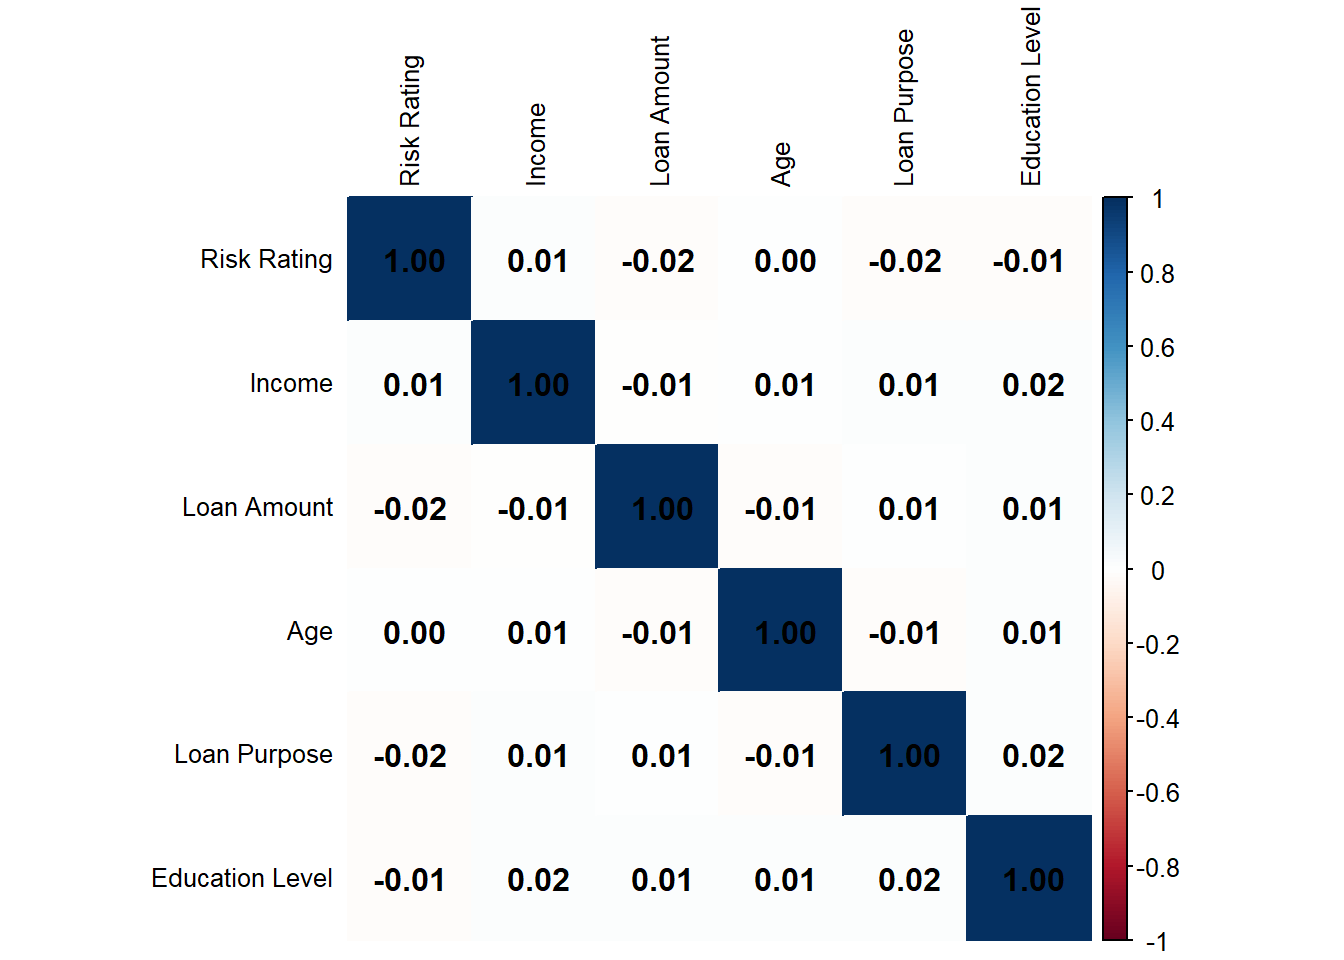
\includegraphics{bitacora_2_files/figure-pdf/unnamed-chunk-12-1.pdf}

Ahora vamos a comenzar a ver los gráficos que se forman de nuestra base
de datos. Para ello vamos analizar cómo es la distribución que siguen
los géneros de nuestra base de datos, esto es solamente por sondear cómo
es nuestra población. Al ser una variable categórica, lo recomendado es
realizar un gráfico de barras.

\begin{Shaded}
\begin{Highlighting}[]
\FunctionTok{library}\NormalTok{(ggplot2)}
\CommentTok{\# Gráfico con las distribuciones del género}
\FunctionTok{ggplot}\NormalTok{(Base\_limpia, }\FunctionTok{aes}\NormalTok{(}\AttributeTok{x =}\NormalTok{ Gender, }\AttributeTok{fill =}\NormalTok{ Gender)) }\SpecialCharTok{+}
  \FunctionTok{geom\_bar}\NormalTok{() }\SpecialCharTok{+}
  \FunctionTok{scale\_fill\_manual}\NormalTok{(}\AttributeTok{values =} \FunctionTok{c}\NormalTok{(}\StringTok{"Male"} \OtherTok{=} \StringTok{"blue"}\NormalTok{, }\StringTok{"Female"} \OtherTok{=} \StringTok{"pink"}\NormalTok{, }\StringTok{"Non{-}binary"} \OtherTok{=} \StringTok{"gray"}\NormalTok{)) }\SpecialCharTok{+}
  \FunctionTok{labs}\NormalTok{(}\AttributeTok{x =} \StringTok{"Distribución de Géneros"}\NormalTok{, }\AttributeTok{y =} \StringTok{"Frecuencia"}\NormalTok{) }\SpecialCharTok{+} \FunctionTok{theme\_minimal}\NormalTok{() }\SpecialCharTok{+}
  \FunctionTok{labs}\NormalTok{(}\AttributeTok{caption =} \StringTok{"Fuente: Elaboración propia utilizando la base de datos de Kaggle"}\NormalTok{) }\SpecialCharTok{+}
\FunctionTok{theme}\NormalTok{(}\AttributeTok{plot.caption =} \FunctionTok{element\_text}\NormalTok{(}\AttributeTok{hjust =} \FloatTok{0.5}\NormalTok{)) }
\end{Highlighting}
\end{Shaded}

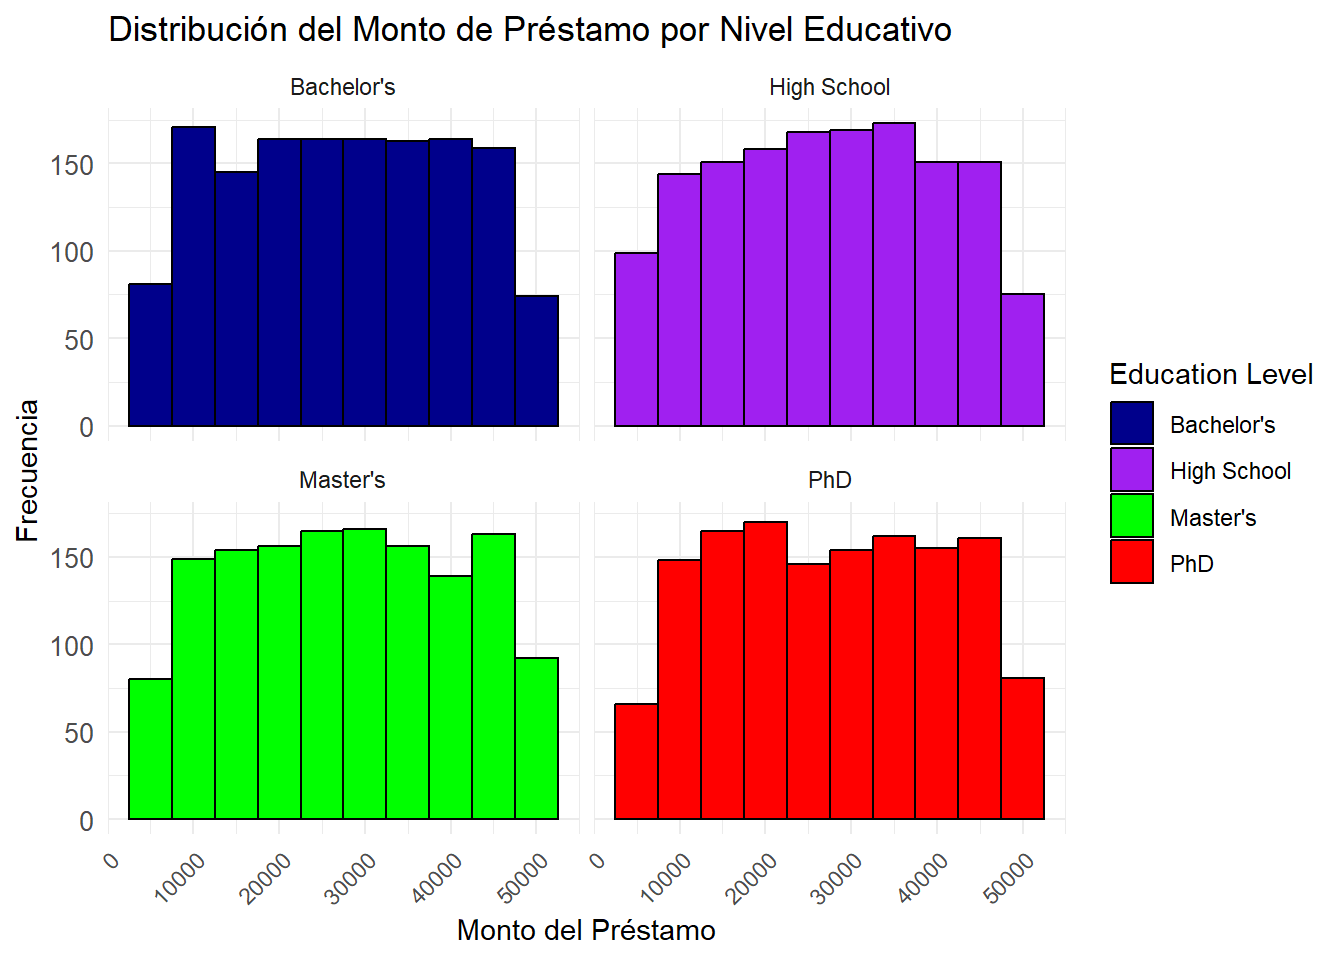
\includegraphics{bitacora_2_files/figure-pdf/unnamed-chunk-13-1.pdf}

Por otro lado, la variable ``Income'', es una variable continua, por lo
que lo recomendado para visualizar la distribución de estos datos de una
manera rápida es a través de los histogramas, por lo que adjuntamos el
gráfico correspondiente:

\begin{Shaded}
\begin{Highlighting}[]
\FunctionTok{library}\NormalTok{(ggplot2)}
\FunctionTok{ggplot}\NormalTok{(Base\_limpia, }\FunctionTok{aes}\NormalTok{(}\AttributeTok{x =}\NormalTok{ Income)) }\SpecialCharTok{+} 
  \FunctionTok{geom\_histogram}\NormalTok{(}\AttributeTok{binwidth =} \DecValTok{10000}\NormalTok{, }\AttributeTok{fill =} \StringTok{"lightblue"}\NormalTok{, }\AttributeTok{color =} \StringTok{"black"}\NormalTok{) }\SpecialCharTok{+} 
  \FunctionTok{labs}\NormalTok{(}\AttributeTok{x =} \StringTok{"Ingreso"}\NormalTok{, }\AttributeTok{y =} \StringTok{"Frecuencia"}\NormalTok{, }\AttributeTok{title =} \StringTok{"Distribución de Ingresos"}\NormalTok{) }\SpecialCharTok{+}
 \FunctionTok{theme\_minimal}\NormalTok{() }\SpecialCharTok{+}
  \FunctionTok{labs}\NormalTok{(}\AttributeTok{caption =} \StringTok{"Fuente: Elaboración propia utilizando la base de datos de Kaggle"}\NormalTok{) }\SpecialCharTok{+}
\FunctionTok{theme}\NormalTok{(}\AttributeTok{plot.caption =} \FunctionTok{element\_text}\NormalTok{(}\AttributeTok{hjust =} \FloatTok{0.5}\NormalTok{)) }
\end{Highlighting}
\end{Shaded}

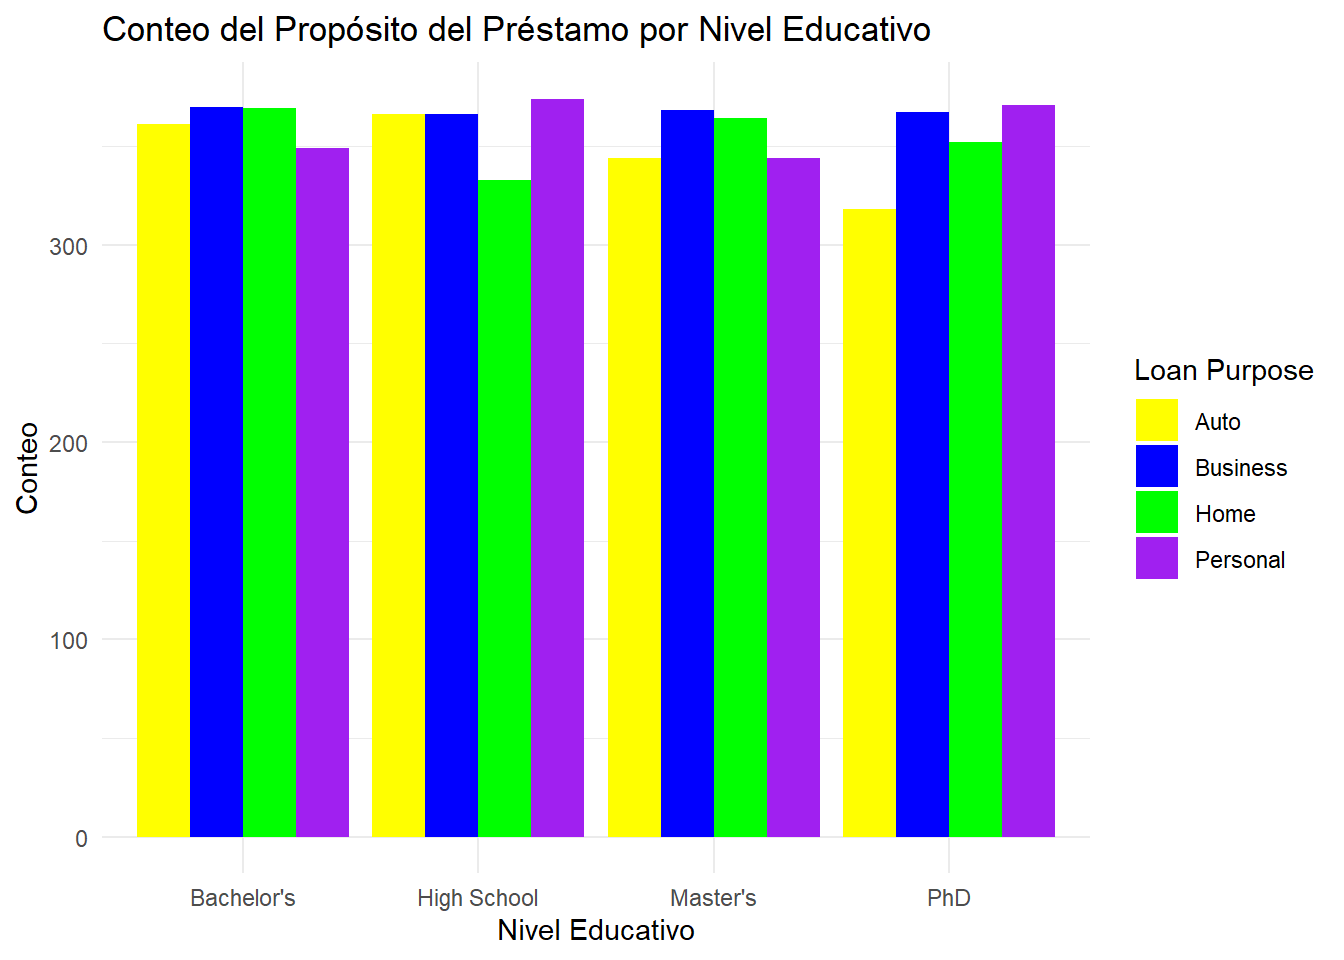
\includegraphics{bitacora_2_files/figure-pdf/unnamed-chunk-14-1.pdf}

Además decidimos realizar un facet en esta misma variable con respecto a
la variable ``Education Level'', con el fin de visualizar la
distribución en cada categoría, esto porque queremos descartar o validar
que de alguna forma el nivel educativo tiene relación con nuestra
variable objetivo, la cual es la calificación de riesgo.

\begin{Shaded}
\begin{Highlighting}[]
\FunctionTok{library}\NormalTok{(ggplot2)}
\FunctionTok{ggplot}\NormalTok{(Base\_limpia, }\FunctionTok{aes}\NormalTok{(}\AttributeTok{x =}\NormalTok{ Income)) }\SpecialCharTok{+} 
  \FunctionTok{geom\_histogram}\NormalTok{(}\AttributeTok{binwidth =} \DecValTok{10000}\NormalTok{, }\AttributeTok{fill =} \StringTok{"lightblue"}\NormalTok{, }\AttributeTok{color =} \StringTok{"black"}\NormalTok{) }\SpecialCharTok{+} 
  \FunctionTok{labs}\NormalTok{(}\AttributeTok{x =} \StringTok{"Ingreso"}\NormalTok{, }\AttributeTok{y =} \StringTok{"Frecuencia"}\NormalTok{, }\AttributeTok{title =} \StringTok{"Distribución de Ingresos"}\NormalTok{) }\SpecialCharTok{+} \FunctionTok{theme\_minimal}\NormalTok{() }\SpecialCharTok{+}
  \FunctionTok{facet\_wrap}\NormalTok{(}\SpecialCharTok{\textasciitilde{}} \StringTok{\textasciigrave{}}\AttributeTok{Education Level}\StringTok{\textasciigrave{}}\NormalTok{) }\SpecialCharTok{+} \CommentTok{\# Facet por nivel educativo}
  \FunctionTok{labs}\NormalTok{(}\AttributeTok{caption =} \StringTok{"Fuente: Elaboración propia utilizando la base de datos de Kaggle"}\NormalTok{) }\SpecialCharTok{+}
\FunctionTok{theme}\NormalTok{(}\AttributeTok{plot.caption =} \FunctionTok{element\_text}\NormalTok{(}\AttributeTok{hjust =} \FloatTok{0.5}\NormalTok{)) }
\end{Highlighting}
\end{Shaded}

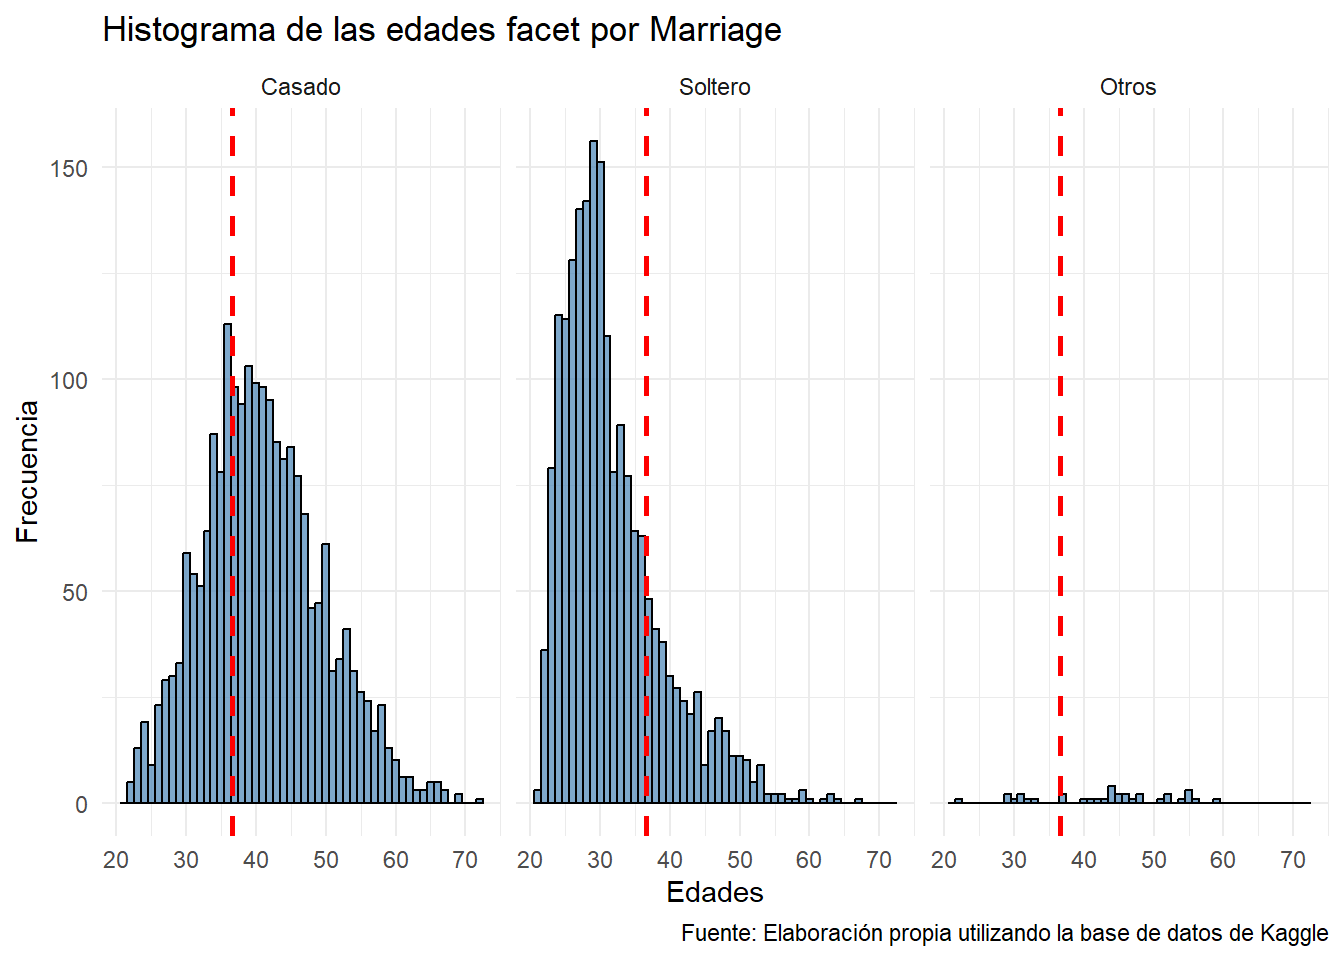
\includegraphics{bitacora_2_files/figure-pdf/unnamed-chunk-15-1.pdf}

Adjuntamos un gráfico más de los ingresos, pero esta vez por género, con
la misma curiosidad de observar cómo es la distribución de estos dada la
mencionada variable.

\begin{Shaded}
\begin{Highlighting}[]
\FunctionTok{library}\NormalTok{(ggplot2)}
\FunctionTok{ggplot}\NormalTok{(Base\_limpia, }\FunctionTok{aes}\NormalTok{(}\AttributeTok{x =}\NormalTok{ Income)) }\SpecialCharTok{+} 
  \FunctionTok{geom\_histogram}\NormalTok{(}\AttributeTok{binwidth =} \DecValTok{10000}\NormalTok{, }\AttributeTok{fill =} \StringTok{"lightblue"}\NormalTok{, }\AttributeTok{color =} \StringTok{"black"}\NormalTok{) }\SpecialCharTok{+} 
  \FunctionTok{labs}\NormalTok{(}\AttributeTok{x =} \StringTok{"Ingreso"}\NormalTok{, }\AttributeTok{y =} \StringTok{"Frecuencia"}\NormalTok{, }\AttributeTok{title =} \StringTok{"Distribución de Ingresos"}\NormalTok{) }\SpecialCharTok{+} \FunctionTok{theme\_minimal}\NormalTok{() }\SpecialCharTok{+}
  \FunctionTok{facet\_wrap}\NormalTok{(}\SpecialCharTok{\textasciitilde{}}\NormalTok{ Gender) }\SpecialCharTok{+} \CommentTok{\# Facet Género}
  \FunctionTok{labs}\NormalTok{(}\AttributeTok{caption =} \StringTok{"Fuente: Elaboración propia utilizando la base de datos de Kaggle"}\NormalTok{) }\SpecialCharTok{+}
\FunctionTok{theme}\NormalTok{(}\AttributeTok{plot.caption =} \FunctionTok{element\_text}\NormalTok{(}\AttributeTok{hjust =} \FloatTok{0.5}\NormalTok{)) }
\end{Highlighting}
\end{Shaded}

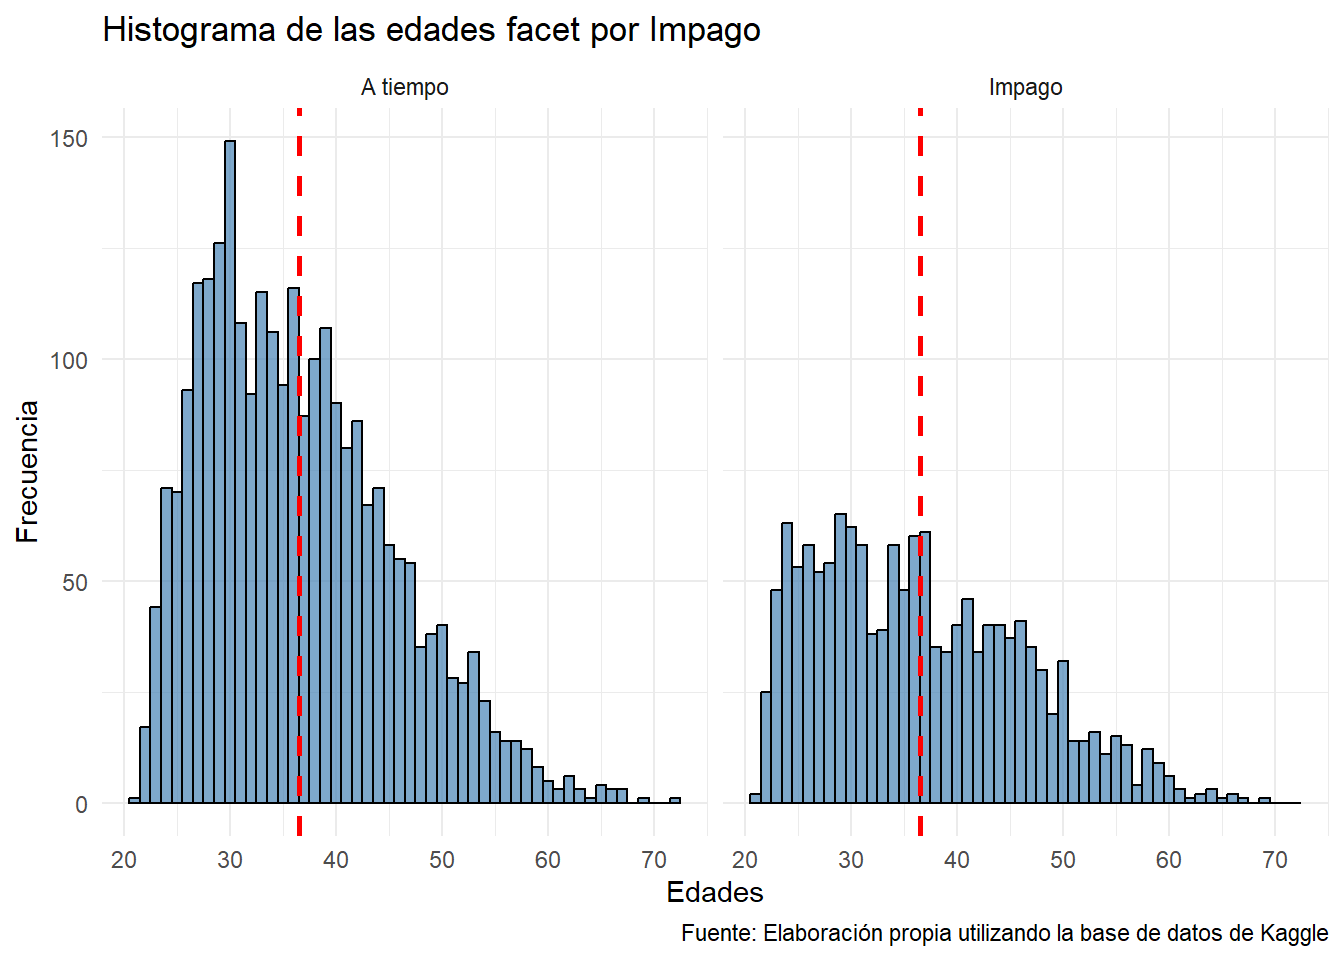
\includegraphics{bitacora_2_files/figure-pdf/unnamed-chunk-16-1.pdf}

Otras variables a tener en cuenta aparte de las anteriores mencionadas
con respecto al riesgo de crédito, son el monto del préstamos y el
propósito del préstamo. Vamos analizar primero el Monto del préstamo,
nos interesa ver qué distribución en general tiene.

\begin{Shaded}
\begin{Highlighting}[]
\FunctionTok{library}\NormalTok{(ggplot2)}

\FunctionTok{ggplot}\NormalTok{(Base\_limpia, }\FunctionTok{aes}\NormalTok{(}\AttributeTok{x =} \StringTok{\textasciigrave{}}\AttributeTok{Loan Amount}\StringTok{\textasciigrave{}}\NormalTok{, }\AttributeTok{fill =}\NormalTok{ Gender)) }\SpecialCharTok{+}  
  \FunctionTok{geom\_histogram}\NormalTok{(}\AttributeTok{binwidth =} \DecValTok{5000}\NormalTok{, }\AttributeTok{color =} \StringTok{"black"}\NormalTok{, }\AttributeTok{position =} \StringTok{"identity"}\NormalTok{) }\SpecialCharTok{+}  
  \FunctionTok{scale\_fill\_manual}\NormalTok{(}\AttributeTok{values =} \FunctionTok{c}\NormalTok{(}\StringTok{"Male"} \OtherTok{=} \StringTok{"darkblue"}\NormalTok{, }\StringTok{"Female"} \OtherTok{=} \StringTok{"purple"}\NormalTok{, }\StringTok{"Non{-}binary"} \OtherTok{=} \StringTok{"green"}\NormalTok{)) }\SpecialCharTok{+}  
  \FunctionTok{facet\_wrap}\NormalTok{(}\SpecialCharTok{\textasciitilde{}}\NormalTok{ Gender) }\SpecialCharTok{+}  
  \FunctionTok{labs}\NormalTok{(}\AttributeTok{x =} \StringTok{"Monto del Préstamo"}\NormalTok{, }\AttributeTok{y =} \StringTok{"Frecuencia"}\NormalTok{, }\AttributeTok{title =} \StringTok{"Distribución del Monto de Préstamo por Género"}\NormalTok{) }\SpecialCharTok{+} 
  \FunctionTok{theme\_minimal}\NormalTok{() }\SpecialCharTok{+}
  \FunctionTok{theme}\NormalTok{(}\AttributeTok{axis.text.y =} \FunctionTok{element\_text}\NormalTok{(}\AttributeTok{size =} \DecValTok{10}\NormalTok{), }\CommentTok{\# Ajustamos el tamaño del texto}
        \AttributeTok{axis.text.x =} \FunctionTok{element\_text}\NormalTok{(}\AttributeTok{angle =} \DecValTok{45}\NormalTok{, }\AttributeTok{hjust =} \DecValTok{1}\NormalTok{)) }\SpecialCharTok{+} \CommentTok{\#Rotamos el texto}
  \FunctionTok{labs}\NormalTok{(}\AttributeTok{caption =} \StringTok{"Fuente: Elaboración propia utilizando la base de datos de Kaggle"}\NormalTok{) }\SpecialCharTok{+}
\FunctionTok{theme}\NormalTok{(}\AttributeTok{plot.caption =} \FunctionTok{element\_text}\NormalTok{(}\AttributeTok{hjust =} \FloatTok{0.5}\NormalTok{)) }
\end{Highlighting}
\end{Shaded}

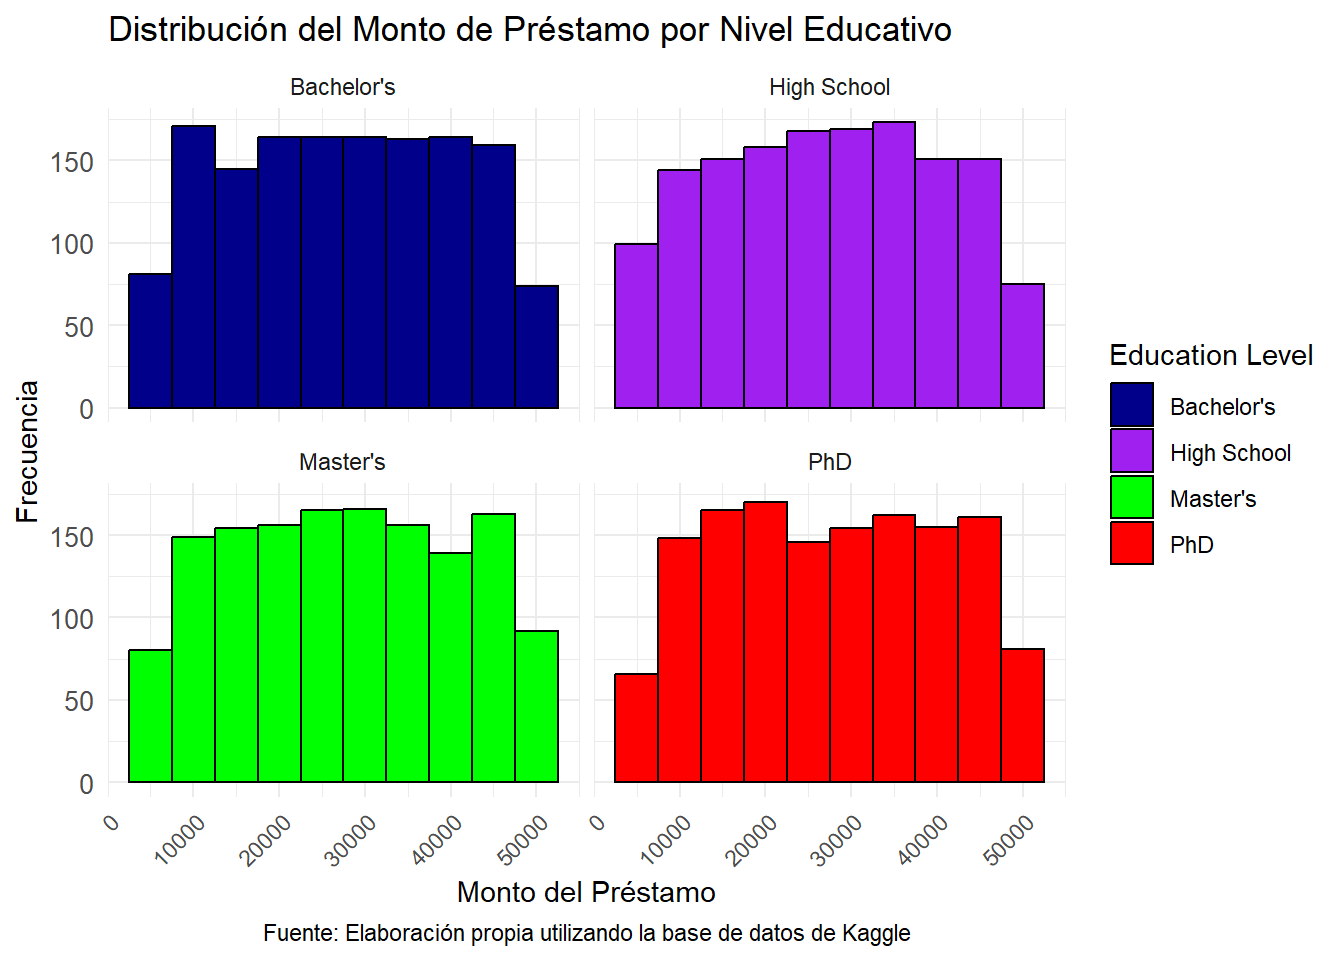
\includegraphics{bitacora_2_files/figure-pdf/unnamed-chunk-17-1.pdf}

Haremos lo mismo, pero esta vez vamos a ver cómo se comportan los
salarios cuando cambiamos la variable y utilizamos por ejemplo el grado
académico.

\begin{Shaded}
\begin{Highlighting}[]
\FunctionTok{library}\NormalTok{(ggplot2)}

\FunctionTok{ggplot}\NormalTok{(Base\_limpia, }\FunctionTok{aes}\NormalTok{(}\AttributeTok{x =} \StringTok{\textasciigrave{}}\AttributeTok{Loan Amount}\StringTok{\textasciigrave{}}\NormalTok{, }\AttributeTok{fill =} \StringTok{\textasciigrave{}}\AttributeTok{Education Level}\StringTok{\textasciigrave{}}\NormalTok{)) }\SpecialCharTok{+}  
  \FunctionTok{geom\_histogram}\NormalTok{(}\AttributeTok{binwidth =} \DecValTok{5000}\NormalTok{, }\AttributeTok{color =} \StringTok{"black"}\NormalTok{, }\AttributeTok{position =} \StringTok{"identity"}\NormalTok{) }\SpecialCharTok{+}  
  \FunctionTok{scale\_fill\_manual}\NormalTok{(}\AttributeTok{values =} \FunctionTok{c}\NormalTok{(}\StringTok{"Bachelor\textquotesingle{}s"} \OtherTok{=} \StringTok{"darkblue"}\NormalTok{, }\StringTok{"High School"} \OtherTok{=} \StringTok{"purple"}\NormalTok{, }\StringTok{"Master\textquotesingle{}s"} \OtherTok{=} \StringTok{"green"}\NormalTok{, }\StringTok{"PhD"} \OtherTok{=} \StringTok{"red"}\NormalTok{)) }\SpecialCharTok{+}  
  \FunctionTok{facet\_wrap}\NormalTok{(}\SpecialCharTok{\textasciitilde{}} \StringTok{\textasciigrave{}}\AttributeTok{Education Level}\StringTok{\textasciigrave{}}\NormalTok{) }\SpecialCharTok{+}  
  \FunctionTok{labs}\NormalTok{(}\AttributeTok{x =} \StringTok{"Monto del Préstamo"}\NormalTok{, }\AttributeTok{y =} \StringTok{"Frecuencia"}\NormalTok{, }\AttributeTok{title =} \StringTok{"Distribución del Monto de Préstamo por Nivel Educativo"}\NormalTok{) }\SpecialCharTok{+} 
  \FunctionTok{theme\_minimal}\NormalTok{() }\SpecialCharTok{+}
  \FunctionTok{theme}\NormalTok{(}\AttributeTok{axis.text.y =} \FunctionTok{element\_text}\NormalTok{(}\AttributeTok{size =} \DecValTok{10}\NormalTok{), }\CommentTok{\# Ajustamos el tamaño del texto}
        \AttributeTok{axis.text.x =} \FunctionTok{element\_text}\NormalTok{(}\AttributeTok{angle =} \DecValTok{45}\NormalTok{, }\AttributeTok{hjust =} \DecValTok{1}\NormalTok{)) }\SpecialCharTok{+} \CommentTok{\#Rotamos el texto}
  \FunctionTok{labs}\NormalTok{(}\AttributeTok{caption =} \StringTok{"Fuente: Elaboración propia utilizando la base de datos de Kaggle"}\NormalTok{) }\SpecialCharTok{+}
\FunctionTok{theme}\NormalTok{(}\AttributeTok{plot.caption =} \FunctionTok{element\_text}\NormalTok{(}\AttributeTok{hjust =} \FloatTok{0.5}\NormalTok{)) }
\end{Highlighting}
\end{Shaded}

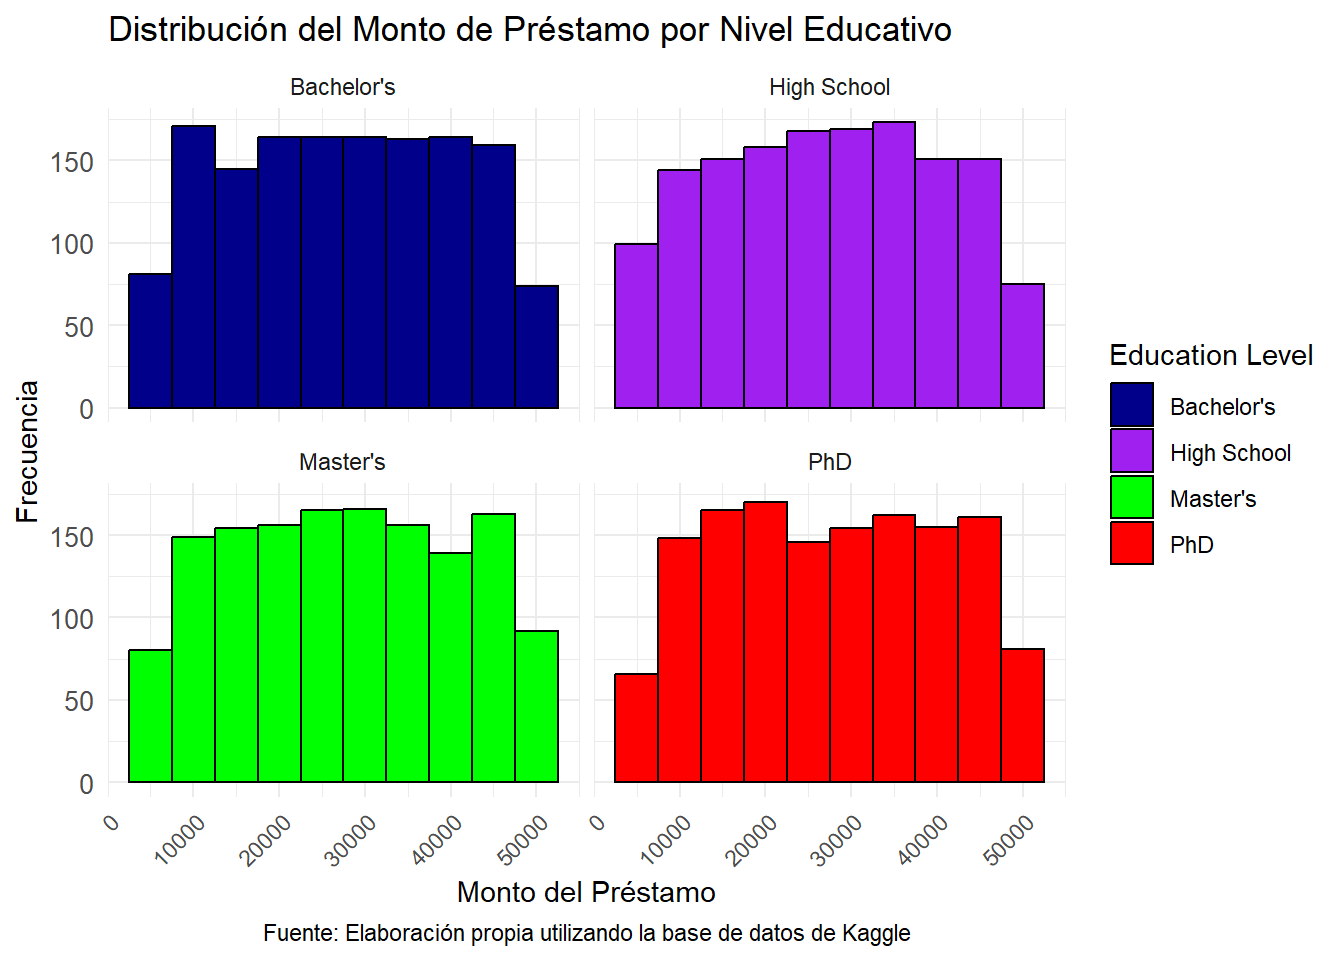
\includegraphics{bitacora_2_files/figure-pdf/unnamed-chunk-18-1.pdf}

Por otro lado, ahora queremos ver el gráfico de la variable propósito
del préstamo en relación con el grado académico, al ser ambas variables
categóricas, lo recomendado es utilizar una geometría que se adapte a
esto, Sin embargo, al ser medidas que están muy cercanas, casi no se
aprecia la diferencia, por lo que se decide adaptarlo a un gráfico de
barras y apreciar mejor la diferencias de manera visual, también
recurrimos al uso de colores, para identificar las variables.

\begin{Shaded}
\begin{Highlighting}[]
\FunctionTok{library}\NormalTok{(ggplot2)}
\FunctionTok{library}\NormalTok{(dplyr)}

\CommentTok{\# Contar las combinaciones de Education Level y Loan Purpose}
\NormalTok{Base\_count }\OtherTok{\textless{}{-}}\NormalTok{ Base\_limpia }\SpecialCharTok{\%\textgreater{}\%}
  \FunctionTok{group\_by}\NormalTok{(}\StringTok{\textasciigrave{}}\AttributeTok{Education Level}\StringTok{\textasciigrave{}}\NormalTok{, }\StringTok{\textasciigrave{}}\AttributeTok{Loan Purpose}\StringTok{\textasciigrave{}}\NormalTok{) }\SpecialCharTok{\%\textgreater{}\%}
  \FunctionTok{summarise}\NormalTok{(}\AttributeTok{Count =} \FunctionTok{n}\NormalTok{(), }\AttributeTok{.groups =} \StringTok{\textquotesingle{}drop\textquotesingle{}}\NormalTok{)}

\CommentTok{\# Gráfico de barras para visualizar el conteo}
\FunctionTok{ggplot}\NormalTok{(Base\_count, }\FunctionTok{aes}\NormalTok{(}\AttributeTok{x =} \StringTok{\textasciigrave{}}\AttributeTok{Education Level}\StringTok{\textasciigrave{}}\NormalTok{, }\AttributeTok{y =}\NormalTok{ Count, }\AttributeTok{fill =} \StringTok{\textasciigrave{}}\AttributeTok{Loan Purpose}\StringTok{\textasciigrave{}}\NormalTok{)) }\SpecialCharTok{+}
  \FunctionTok{geom\_bar}\NormalTok{(}\AttributeTok{stat =} \StringTok{"identity"}\NormalTok{, }\AttributeTok{position =} \StringTok{"dodge"}\NormalTok{) }\SpecialCharTok{+}  \CommentTok{\# Usa barras para mostrar el conteo}
  \FunctionTok{labs}\NormalTok{(}\AttributeTok{x =} \StringTok{"Nivel Educativo"}\NormalTok{, }\AttributeTok{y =} \StringTok{"Conteo"}\NormalTok{, }\AttributeTok{title =} \StringTok{"Conteo del Propósito del Préstamo por Nivel Educativo"}\NormalTok{) }\SpecialCharTok{+}
  \FunctionTok{scale\_fill\_manual}\NormalTok{(}\AttributeTok{values =} \FunctionTok{c}\NormalTok{(}\StringTok{"Business"} \OtherTok{=} \StringTok{"blue"}\NormalTok{, }\StringTok{"Personal"} \OtherTok{=} \StringTok{"purple"}\NormalTok{, }\StringTok{"Home"} \OtherTok{=} \StringTok{"green"}\NormalTok{, }\StringTok{"Auto"} \OtherTok{=} \StringTok{"yellow"}\NormalTok{)) }\SpecialCharTok{+}
  \FunctionTok{theme\_minimal}\NormalTok{() }\SpecialCharTok{+}
  \FunctionTok{labs}\NormalTok{(}\AttributeTok{caption =} \StringTok{"Fuente: Elaboración propia utilizando la base de datos de Kaggle"}\NormalTok{) }\SpecialCharTok{+}
\FunctionTok{theme}\NormalTok{(}\AttributeTok{plot.caption =} \FunctionTok{element\_text}\NormalTok{(}\AttributeTok{hjust =} \FloatTok{0.5}\NormalTok{)) }
\end{Highlighting}
\end{Shaded}

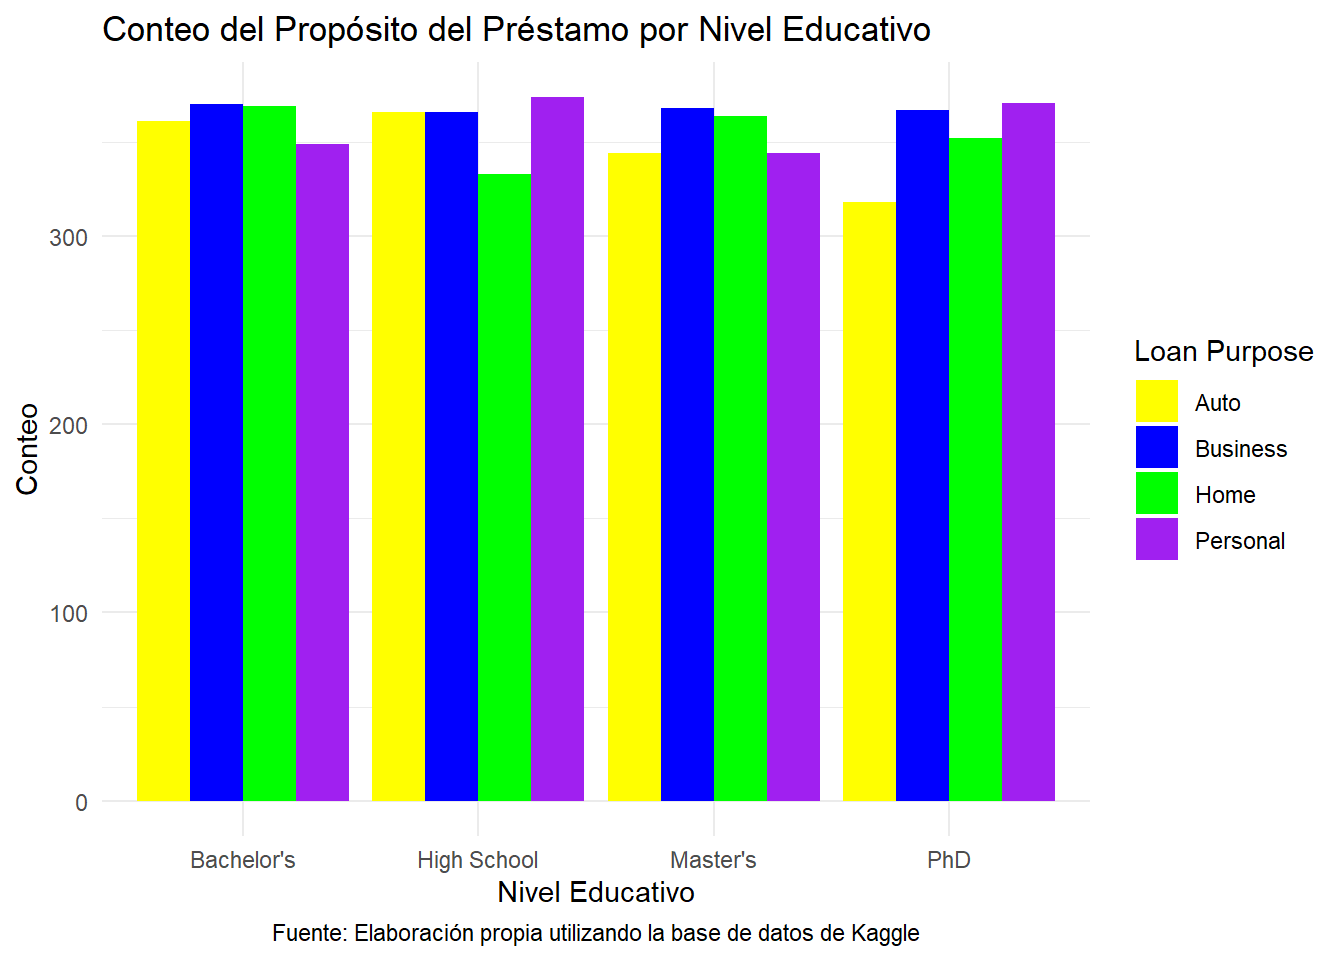
\includegraphics{bitacora_2_files/figure-pdf/unnamed-chunk-19-1.pdf}

Para terminar esta sección, vamos a graficar con la variable objetivo de
interés, la cual es la Calificación de riesgo, para ello, lo vamos a
comparar a través de diversos gráficos con las variables de nivel
educativo, ingresos, monto del préstamo, edad y género. Es importante
mencionar, que las variables en conjunto afectan a esta calificación, al
menos así es de manera teórica. En este apartado nos vamos a centrar en
estos gráficos, en secciones posteriores nos ecargaremos de hacer la
conexión entre la teoría, nuestras hipótesis y los datos obtenidos.

Para comenzar, nos interesa observar cómo se comporta la variable de
Calificación de Riesgo, con respecto a la edad:

\begin{Shaded}
\begin{Highlighting}[]
\FunctionTok{library}\NormalTok{(ggplot2)}
\FunctionTok{ggplot}\NormalTok{(Base\_limpia, }\FunctionTok{aes}\NormalTok{(}\AttributeTok{x =}\NormalTok{ Age, }\AttributeTok{fill =} \StringTok{\textasciigrave{}}\AttributeTok{Risk Rating}\StringTok{\textasciigrave{}}\NormalTok{)) }\SpecialCharTok{+}
  \FunctionTok{geom\_bar}\NormalTok{() }\SpecialCharTok{+}  
  \FunctionTok{labs}\NormalTok{(}\AttributeTok{x =} \StringTok{"Edad"}\NormalTok{, }\AttributeTok{y =} \StringTok{"Conteo"}\NormalTok{, }\AttributeTok{title =} \StringTok{"Distribución de Calificación de Riesgo por Edad"}\NormalTok{) }\SpecialCharTok{+} 
  \FunctionTok{theme\_minimal}\NormalTok{() }\SpecialCharTok{+}  
  \FunctionTok{scale\_fill\_brewer}\NormalTok{(}\AttributeTok{palette =} \StringTok{"Set1"}\NormalTok{)  }\SpecialCharTok{+}
  \FunctionTok{labs}\NormalTok{(}\AttributeTok{caption =} \StringTok{"Fuente: Elaboración propia utilizando la base de datos de Kaggle"}\NormalTok{) }\SpecialCharTok{+}
\FunctionTok{theme}\NormalTok{(}\AttributeTok{plot.caption =} \FunctionTok{element\_text}\NormalTok{(}\AttributeTok{hjust =} \FloatTok{0.5}\NormalTok{)) }
\end{Highlighting}
\end{Shaded}

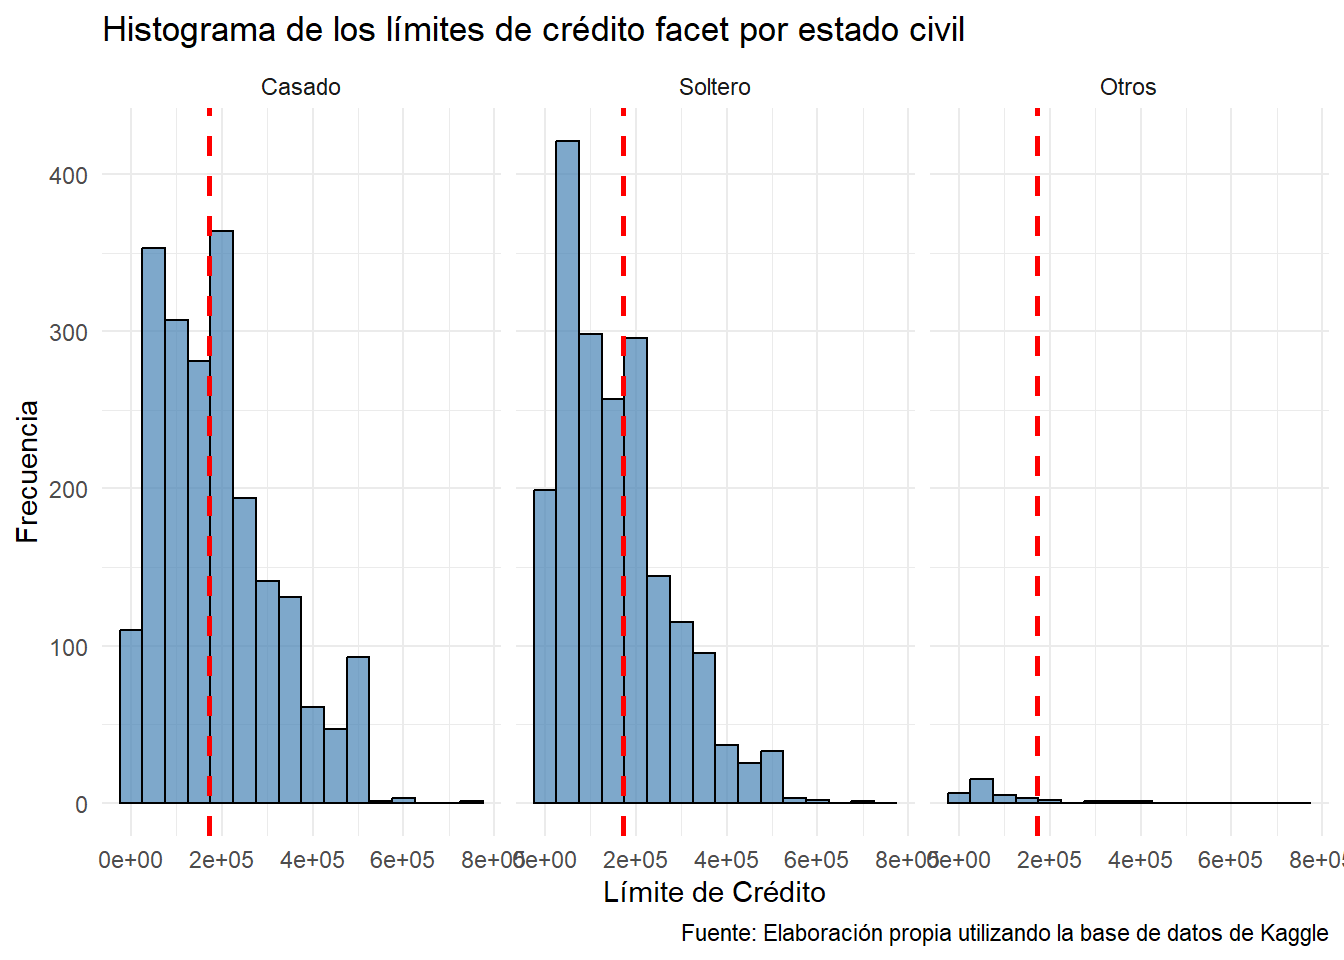
\includegraphics{bitacora_2_files/figure-pdf/unnamed-chunk-20-1.pdf}

Por otro lado, vamos a ver cómo se comporta la distribución de la
calificación de riesgo, haciendo un facet con la categoría Nivel
Educativo. Al ser dos variables categóricas las que estamos comparando,
lo recomendado es utilizar un gráfico de barras.

\begin{Shaded}
\begin{Highlighting}[]
\FunctionTok{library}\NormalTok{(ggplot2)}

\FunctionTok{ggplot}\NormalTok{(Base\_limpia, }\FunctionTok{aes}\NormalTok{(}\AttributeTok{x =} \StringTok{\textasciigrave{}}\AttributeTok{Risk Rating}\StringTok{\textasciigrave{}}\NormalTok{, }\AttributeTok{fill =} \StringTok{\textasciigrave{}}\AttributeTok{Education Level}\StringTok{\textasciigrave{}}\NormalTok{)) }\SpecialCharTok{+}  
  \FunctionTok{geom\_bar}\NormalTok{(}\AttributeTok{color =} \StringTok{"black"}\NormalTok{, }\AttributeTok{position =} \StringTok{"identity"}\NormalTok{) }\SpecialCharTok{+}  
  \FunctionTok{scale\_fill\_manual}\NormalTok{(}\AttributeTok{values =} \FunctionTok{c}\NormalTok{(}\StringTok{"Bachelor\textquotesingle{}s"} \OtherTok{=} \StringTok{"darkblue"}\NormalTok{, }\StringTok{"High School"} \OtherTok{=} \StringTok{"purple"}\NormalTok{, }\StringTok{"Master\textquotesingle{}s"} \OtherTok{=} \StringTok{"green"}\NormalTok{, }\StringTok{"PhD"} \OtherTok{=} \StringTok{"red"}\NormalTok{)) }\SpecialCharTok{+}  
  \FunctionTok{facet\_wrap}\NormalTok{(}\SpecialCharTok{\textasciitilde{}} \StringTok{\textasciigrave{}}\AttributeTok{Education Level}\StringTok{\textasciigrave{}}\NormalTok{) }\SpecialCharTok{+}  
  \FunctionTok{labs}\NormalTok{(}\AttributeTok{x =} \StringTok{"Calificación de Riesgo"}\NormalTok{, }\AttributeTok{y =} \StringTok{"Frecuencia"}\NormalTok{, }\AttributeTok{title =} \StringTok{"Distribución de la Calificación de Riesgo por Nivel Educativo"}\NormalTok{) }\SpecialCharTok{+} 
  \FunctionTok{theme\_minimal}\NormalTok{() }\SpecialCharTok{+}
  \FunctionTok{theme}\NormalTok{(}\AttributeTok{axis.text.y =} \FunctionTok{element\_text}\NormalTok{(}\AttributeTok{size =} \DecValTok{10}\NormalTok{), }\CommentTok{\# Ajustamos el tamaño del texto}
        \AttributeTok{axis.text.x =} \FunctionTok{element\_text}\NormalTok{(}\AttributeTok{angle =} \DecValTok{45}\NormalTok{, }\AttributeTok{hjust =} \DecValTok{1}\NormalTok{)) }\SpecialCharTok{+} \CommentTok{\# Rotamos el texto}
  \FunctionTok{labs}\NormalTok{(}\AttributeTok{caption =} \StringTok{"Fuente: Elaboración propia utilizando la base de datos de Kaggle"}\NormalTok{) }\SpecialCharTok{+}
\FunctionTok{theme}\NormalTok{(}\AttributeTok{plot.caption =} \FunctionTok{element\_text}\NormalTok{(}\AttributeTok{hjust =} \FloatTok{0.5}\NormalTok{)) }
\end{Highlighting}
\end{Shaded}

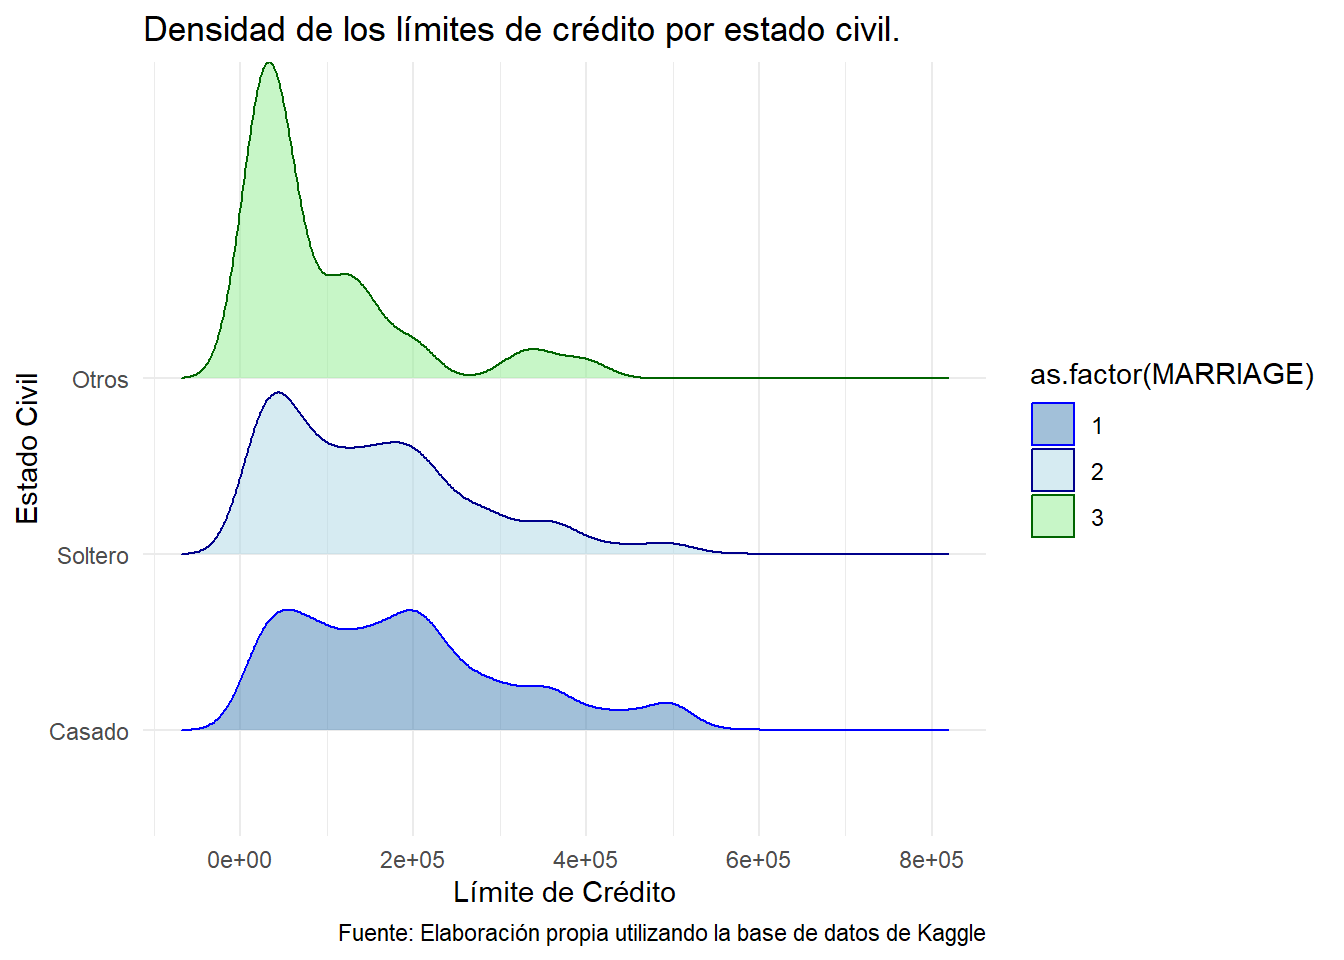
\includegraphics{bitacora_2_files/figure-pdf/unnamed-chunk-21-1.pdf}

A su vez, nos interesa observar cómo se ve el gráifco de la variable
calificación de riesgo con la variable contra la variable ingreso. Para
este gráfico, vamos a utilizar el recomendado en las notas del profesor
Maikol Solís, el cual indica que usar diagramas de cajas es útil para
comparar las distribuciones.

\begin{Shaded}
\begin{Highlighting}[]
\FunctionTok{library}\NormalTok{(ggplot2)}

\FunctionTok{ggplot}\NormalTok{(Base\_limpia, }\FunctionTok{aes}\NormalTok{(}\AttributeTok{x =} \StringTok{\textasciigrave{}}\AttributeTok{Risk Rating}\StringTok{\textasciigrave{}}\NormalTok{, }\AttributeTok{y =}\NormalTok{ Income, }\AttributeTok{fill =} \StringTok{\textasciigrave{}}\AttributeTok{Risk Rating}\StringTok{\textasciigrave{}}\NormalTok{)) }\SpecialCharTok{+}  
  \FunctionTok{geom\_boxplot}\NormalTok{(}\AttributeTok{color =} \StringTok{"black"}\NormalTok{) }\SpecialCharTok{+}  
  \FunctionTok{scale\_fill\_manual}\NormalTok{(}\AttributeTok{values =} \FunctionTok{c}\NormalTok{(}\StringTok{"Low"} \OtherTok{=} \StringTok{"green"}\NormalTok{, }\StringTok{"Medium"} \OtherTok{=} \StringTok{"yellow"}\NormalTok{, }\StringTok{"High"} \OtherTok{=} \StringTok{"red"}\NormalTok{, }\StringTok{"Very High"} \OtherTok{=} \StringTok{"purple"}\NormalTok{)) }\SpecialCharTok{+}  
  \FunctionTok{labs}\NormalTok{(}\AttributeTok{x =} \StringTok{"Calificación de Riesgo"}\NormalTok{, }\AttributeTok{y =} \StringTok{"Ingreso"}\NormalTok{, }\AttributeTok{title =} \StringTok{"Comparación de la Calificación de Riesgo con el Ingreso"}\NormalTok{) }\SpecialCharTok{+} 
  \FunctionTok{theme\_minimal}\NormalTok{() }\SpecialCharTok{+}
  \FunctionTok{theme}\NormalTok{(}\AttributeTok{axis.text.y =} \FunctionTok{element\_text}\NormalTok{(}\AttributeTok{size =} \DecValTok{10}\NormalTok{), }\CommentTok{\# Ajustamos el tamaño del texto}
        \AttributeTok{axis.text.x =} \FunctionTok{element\_text}\NormalTok{(}\AttributeTok{angle =} \DecValTok{45}\NormalTok{, }\AttributeTok{hjust =} \DecValTok{1}\NormalTok{))  }\SpecialCharTok{+}\CommentTok{\# Rotamos el texto}
  \FunctionTok{labs}\NormalTok{(}\AttributeTok{caption =} \StringTok{"Fuente: Elaboración propia utilizando la base de datos de Kaggle"}\NormalTok{) }\SpecialCharTok{+}
\FunctionTok{theme}\NormalTok{(}\AttributeTok{plot.caption =} \FunctionTok{element\_text}\NormalTok{(}\AttributeTok{hjust =} \FloatTok{0.5}\NormalTok{)) }
\end{Highlighting}
\end{Shaded}

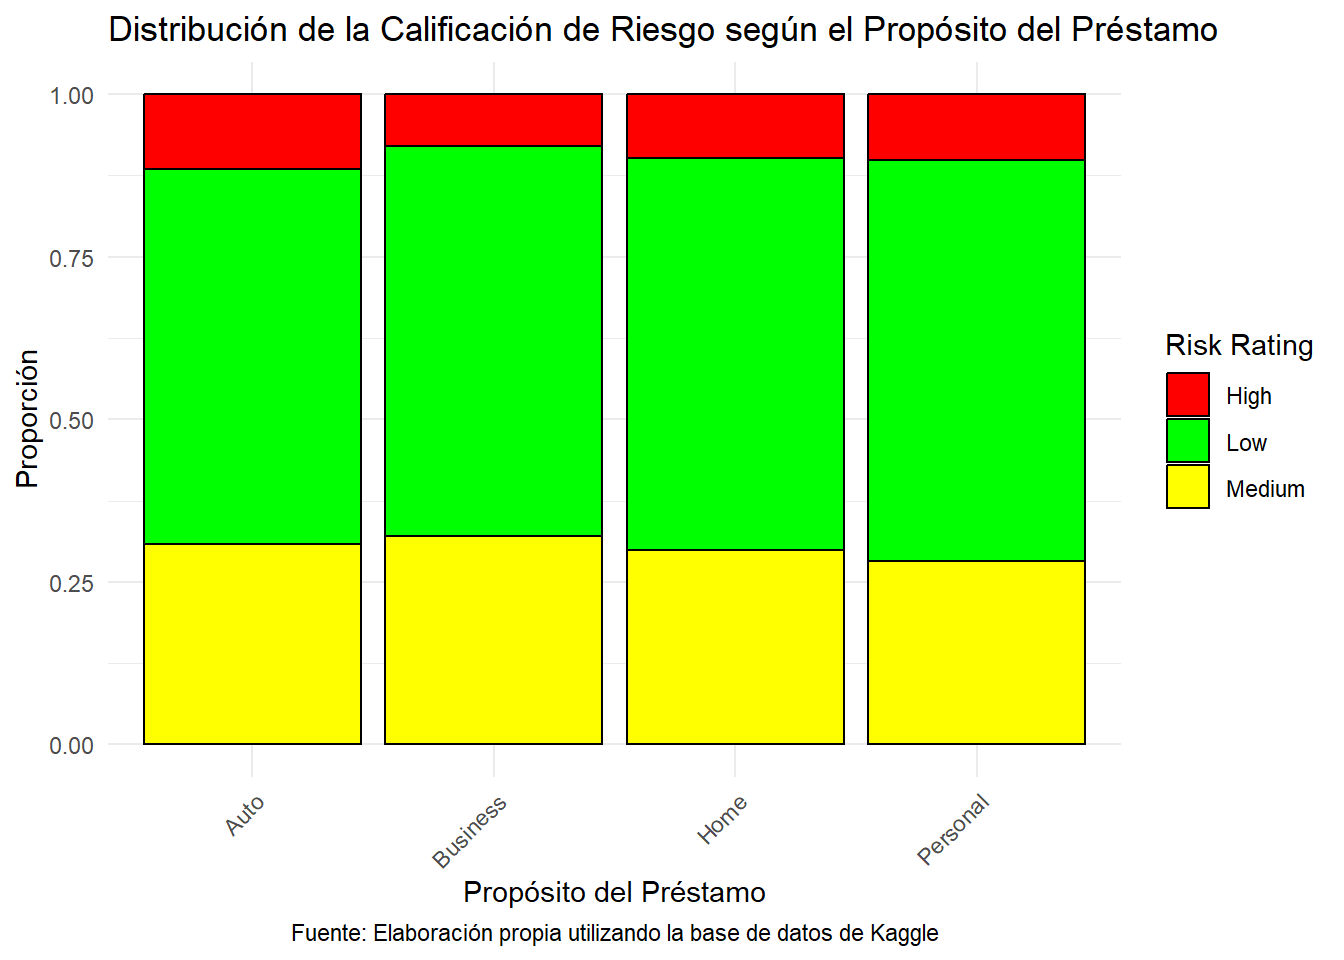
\includegraphics{bitacora_2_files/figure-pdf/unnamed-chunk-22-1.pdf}

Otra de las variables de interés, es la calificación de riesgo contra el
propósito del préstamo.

\begin{Shaded}
\begin{Highlighting}[]
\FunctionTok{library}\NormalTok{(ggplot2)}

\FunctionTok{ggplot}\NormalTok{(Base\_limpia, }\FunctionTok{aes}\NormalTok{(}\AttributeTok{x =} \StringTok{\textasciigrave{}}\AttributeTok{Loan Purpose}\StringTok{\textasciigrave{}}\NormalTok{, }\AttributeTok{fill =} \StringTok{\textasciigrave{}}\AttributeTok{Risk Rating}\StringTok{\textasciigrave{}}\NormalTok{)) }\SpecialCharTok{+}  
  \FunctionTok{geom\_bar}\NormalTok{(}\AttributeTok{position =} \StringTok{"fill"}\NormalTok{, }\AttributeTok{color =} \StringTok{"black"}\NormalTok{) }\SpecialCharTok{+}  
  \FunctionTok{scale\_fill\_manual}\NormalTok{(}\AttributeTok{values =} \FunctionTok{c}\NormalTok{(}\StringTok{"Low"} \OtherTok{=} \StringTok{"green"}\NormalTok{, }\StringTok{"Medium"} \OtherTok{=} \StringTok{"yellow"}\NormalTok{, }\StringTok{"High"} \OtherTok{=} \StringTok{"red"}\NormalTok{, }\StringTok{"Very High"} \OtherTok{=} \StringTok{"purple"}\NormalTok{)) }\SpecialCharTok{+}  
  \FunctionTok{labs}\NormalTok{(}\AttributeTok{x =} \StringTok{"Propósito del Préstamo"}\NormalTok{, }\AttributeTok{y =} \StringTok{"Proporción"}\NormalTok{, }\AttributeTok{title =} \StringTok{"Distribución de la Calificación de Riesgo según el Propósito del Préstamo"}\NormalTok{) }\SpecialCharTok{+} 
  \FunctionTok{theme\_minimal}\NormalTok{() }\SpecialCharTok{+}
  \FunctionTok{theme}\NormalTok{(}\AttributeTok{axis.text.x =} \FunctionTok{element\_text}\NormalTok{(}\AttributeTok{angle =} \DecValTok{45}\NormalTok{, }\AttributeTok{hjust =} \DecValTok{1}\NormalTok{)) }\SpecialCharTok{+} \CommentTok{\# Rotamos el texto para mejorar la legibilidad}
  \FunctionTok{labs}\NormalTok{(}\AttributeTok{caption =} \StringTok{"Fuente: Elaboración propia utilizando la base de datos de Kaggle"}\NormalTok{) }\SpecialCharTok{+}
\FunctionTok{theme}\NormalTok{(}\AttributeTok{plot.caption =} \FunctionTok{element\_text}\NormalTok{(}\AttributeTok{hjust =} \FloatTok{0.5}\NormalTok{)) }
\end{Highlighting}
\end{Shaded}

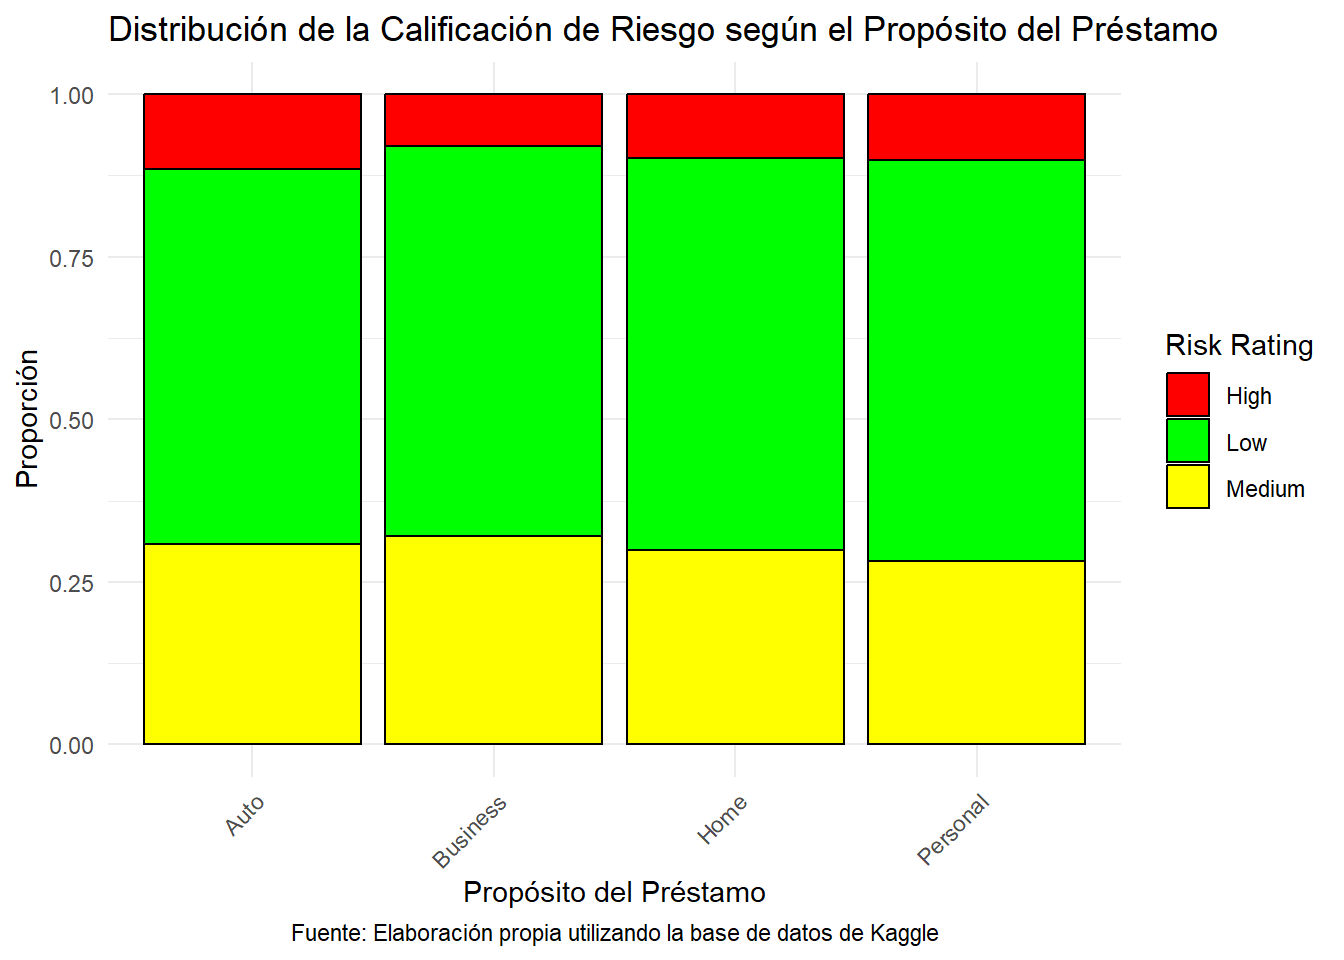
\includegraphics{bitacora_2_files/figure-pdf/unnamed-chunk-23-1.pdf}

Por último, vamos a ver la distribución que existe de la variable
calificación de riesgo cuando la comparamos contra el monto del
préstamo.

\begin{Shaded}
\begin{Highlighting}[]
\FunctionTok{library}\NormalTok{(ggplot2)}

\FunctionTok{ggplot}\NormalTok{(Base\_limpia, }\FunctionTok{aes}\NormalTok{(}\AttributeTok{x =} \StringTok{\textasciigrave{}}\AttributeTok{Risk Rating}\StringTok{\textasciigrave{}}\NormalTok{, }\AttributeTok{y =} \StringTok{\textasciigrave{}}\AttributeTok{Loan Amount}\StringTok{\textasciigrave{}}\NormalTok{, }\AttributeTok{fill =} \StringTok{\textasciigrave{}}\AttributeTok{Risk Rating}\StringTok{\textasciigrave{}}\NormalTok{)) }\SpecialCharTok{+}  
  \FunctionTok{geom\_boxplot}\NormalTok{(}\AttributeTok{color =} \StringTok{"black"}\NormalTok{) }\SpecialCharTok{+}  
  \FunctionTok{scale\_fill\_manual}\NormalTok{(}\AttributeTok{values =} \FunctionTok{c}\NormalTok{(}\StringTok{"Low"} \OtherTok{=} \StringTok{"green"}\NormalTok{, }\StringTok{"Medium"} \OtherTok{=} \StringTok{"yellow"}\NormalTok{, }\StringTok{"High"} \OtherTok{=} \StringTok{"red"}\NormalTok{, }\StringTok{"Very High"} \OtherTok{=} \StringTok{"purple"}\NormalTok{)) }\SpecialCharTok{+}  
  \FunctionTok{labs}\NormalTok{(}\AttributeTok{x =} \StringTok{"Calificación de Riesgo"}\NormalTok{, }\AttributeTok{y =} \StringTok{"Monto del Préstamo"}\NormalTok{, }\AttributeTok{title =} \StringTok{"Comparación de la Calificación de Riesgo con el Monto del Préstamo"}\NormalTok{) }\SpecialCharTok{+} 
  \FunctionTok{theme\_minimal}\NormalTok{() }\SpecialCharTok{+}
  \FunctionTok{theme}\NormalTok{(}\AttributeTok{axis.text.y =} \FunctionTok{element\_text}\NormalTok{(}\AttributeTok{size =} \DecValTok{10}\NormalTok{), }\CommentTok{\# Ajustamos el tamaño del texto}
        \AttributeTok{axis.text.x =} \FunctionTok{element\_text}\NormalTok{(}\AttributeTok{angle =} \DecValTok{45}\NormalTok{, }\AttributeTok{hjust =} \DecValTok{1}\NormalTok{))  }\SpecialCharTok{+} \CommentTok{\# Rotamos el texto }
\FunctionTok{labs}\NormalTok{(}\AttributeTok{caption =} \StringTok{"Fuente: Elaboración propia utilizando la base de datos de Kaggle"}\NormalTok{) }\SpecialCharTok{+}
\FunctionTok{theme}\NormalTok{(}\AttributeTok{plot.caption =} \FunctionTok{element\_text}\NormalTok{(}\AttributeTok{hjust =} \FloatTok{0.5}\NormalTok{)) }
\end{Highlighting}
\end{Shaded}

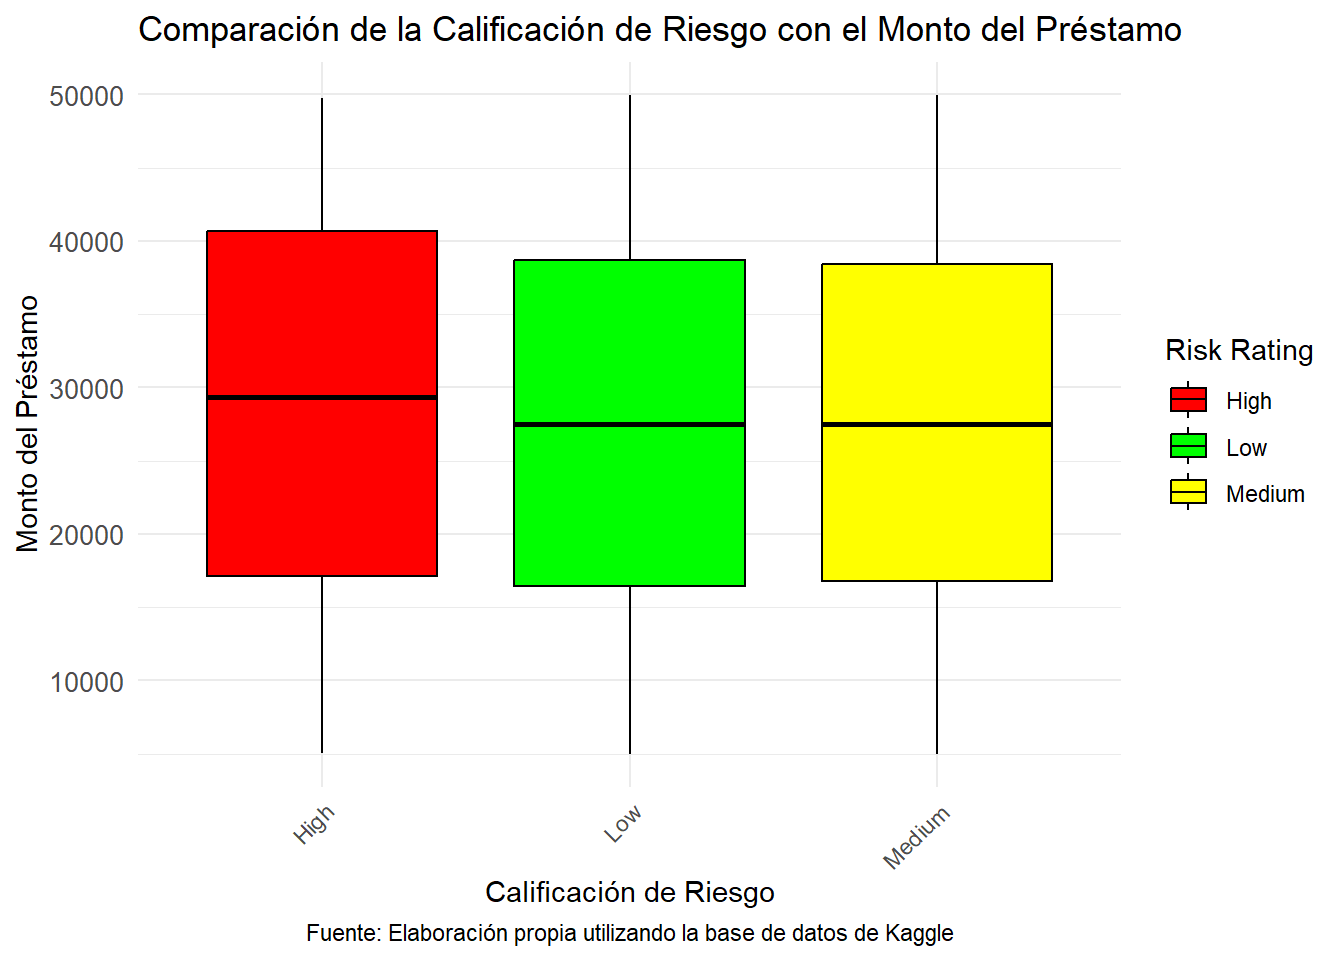
\includegraphics{bitacora_2_files/figure-pdf/unnamed-chunk-24-1.pdf}

\section{Propuesta Metodológica}\label{propuesta-metodoluxf3gica}

se utilizan los gráficos, como ayuda en las distribuciones de las
variables, con el fin de observar su comportamiento. Sin embargo, hay
que hacer un análisis más a profundidad, para ello utilizamos el
coeficiente de correlación de Pearson, que fue justo el que utilizamos
para crear nuestra matriz de correlación, a continuación enunciamos el
proceso teórico de dicho procedimiento.

Como menciona el autor (Edgar Apaza 2022) ``Los análisis de correlación
son métodos estadísticos descriptivos utilizados en investigación de
nivel relacional, con los que estima la magnitud y define la tendencia
de la relación entre variables.''. Como queremos encontrar alguna
relación en nuestra variables de interés, entonces queremos utilizar
esta metodología para encontrar dicha relación. Según este mismo autor
``el método de correlación de Pearson es una técnica bivariada que
emplea en circunstancia multivariada para la explicación de diversos
fenómenos relacionados en el campo animal y vegetal. En la correlación
de Pearson, los procedimientos guardan relación con la naturaleza de las
variables utilizadas.''. Como podemos observar el método nos sirve para
este estudio, pues tenemos muchas variables, pero el índice sale de
comparar dos a dos las variables, para obtener la correlación entre
ellas, lo que luego acomodamos en una matriz para tener una mejor
observación de ellas.

R ya posee una librería que calcula automáticamente este coeficiente,
sin embargo, la manera teórica de hacerlo es mediante la fórmula:

\(\rho = \frac{\sigma_{XY}}{\sigma_X \sigma_Y}\)

En donde \(\rho\) recibe el nombre de Coeficiente de correlación de
Pearson y además tiene que ocurrir que \(-1 \leq \rho \leq 1\). Según el
autor (Edgar Apaza 2022) ``\ldots{} se deduce la magnitud de la relación
lineal entre variables, los que pueden ser calificados como: Correlación
Nula (0), Muy baja (0.01 a 0.1), Débil (0.11 a 0.5), Media (0.51 a
0.75), considerable (0.76 a 0.9), Muy fuerte (0.91 a 0.99) y
Perfecta(1)''. Otro aspecto importante a decir acerca de nuestro estudio
y que tiene relación con lo que este mismo autor afirma y es que
``\rho = 0.000, no necesariamente implica que no exista relación entre
las varables, sino que la relación podría ser no lineal''. Esto de hecho
es un buen punto en vista de los resultados que arrojó nuestra matriz de
correlación. Además, algo que deberíamos de tomar en cuenta, es que
estamos trabajando con variables categóricas, a la hora de la conversión
puede haber fuga de información, por ello hay que tener cuidado con solo
ver una cifra y animarse a dar una conclusión, cuando en realidad hay
que analizar a detalle qué es lo que está pasando.

\section{Construcción de Fichas de
Resultados}\label{construcciuxf3n-de-fichas-de-resultados}

\begin{Shaded}
\begin{Highlighting}[]
\ControlFlowTok{if}\NormalTok{ (}\SpecialCharTok{!}\FunctionTok{requireNamespace}\NormalTok{(}\StringTok{"kableExtra"}\NormalTok{, }\AttributeTok{quietly =} \ConstantTok{TRUE}\NormalTok{)) \{}
  \FunctionTok{install.packages}\NormalTok{(}\StringTok{"kableExtra"}\NormalTok{)}
\NormalTok{\}}
\FunctionTok{library}\NormalTok{(kableExtra)}


\NormalTok{data }\OtherTok{\textless{}{-}} \FunctionTok{data.frame}\NormalTok{(}
  \AttributeTok{Encabezado =} \FunctionTok{c}\NormalTok{(}\StringTok{"Nombre de Su hallazgo"}\NormalTok{, }
                 \StringTok{"Resumen en una Oración"}\NormalTok{, }
                 \StringTok{"Problemas o Posibles Desafíos"}\NormalTok{, }
                 \StringTok{"Resumen en un párrafo"}\NormalTok{),}
  \AttributeTok{Contenido =} \FunctionTok{c}\NormalTok{(}\StringTok{"Poca Correlación entre las variables."}\NormalTok{, }
                \StringTok{"Encontramos que las variables a utilizar no presentan una correlación fuerte, según el índice de Pearson."}\NormalTok{, }
                \StringTok{"La conversión de variable categórica a variable numérica puede estar afectando al resultado. Además, podría ser que la relación entre las variables en realidad no es lineal."}\NormalTok{, }
                \StringTok{"Al utilizar el índice de correlación de Pearson, hay que utilizar variables numéricas, por lo que se utiliza una conversión de las variables categóricas a variables numéricas para poder realizar dicho cálculo, sin embargo se encuentra que las variables no están teniendo una relación, al menos de manera lineal que es lo que calcula dicho índice."}\NormalTok{)}
\NormalTok{)}


\ControlFlowTok{if}\NormalTok{ (knitr}\SpecialCharTok{::}\FunctionTok{is\_html\_output}\NormalTok{()) \{}
  \CommentTok{\# Si es HTML}
  \FunctionTok{kable}\NormalTok{(data, }\AttributeTok{col.names =} \FunctionTok{c}\NormalTok{(}\StringTok{"Encabezado"}\NormalTok{, }\StringTok{"Contenido"}\NormalTok{), }
        \AttributeTok{format =} \StringTok{"html"}\NormalTok{, }
        \AttributeTok{escape =} \ConstantTok{FALSE}\NormalTok{) }\SpecialCharTok{\%\textgreater{}\%}
    \FunctionTok{kable\_styling}\NormalTok{(}\AttributeTok{full\_width =} \ConstantTok{FALSE}\NormalTok{) }\SpecialCharTok{\%\textgreater{}\%}
    \FunctionTok{add\_header\_above}\NormalTok{(}\FunctionTok{c}\NormalTok{(}\StringTok{"Hallazgo de Resultado 1"} \OtherTok{=} \DecValTok{2}\NormalTok{), }\AttributeTok{bold =} \ConstantTok{TRUE}\NormalTok{)}
\NormalTok{\} }\ControlFlowTok{else}\NormalTok{ \{}
  \CommentTok{\# Si es PDF}
  \FunctionTok{kable}\NormalTok{(data, }\AttributeTok{col.names =} \FunctionTok{c}\NormalTok{(}\StringTok{"Encabezado"}\NormalTok{, }\StringTok{"Contenido"}\NormalTok{), }
        \AttributeTok{format =} \StringTok{"latex"}\NormalTok{, }
        \AttributeTok{booktabs =} \ConstantTok{TRUE}\NormalTok{) }\SpecialCharTok{\%\textgreater{}\%}
    \FunctionTok{kable\_styling}\NormalTok{(}\AttributeTok{latex\_options =} \FunctionTok{c}\NormalTok{(}\StringTok{"striped"}\NormalTok{, }\StringTok{"hold\_position"}\NormalTok{))}
\NormalTok{\}}
\end{Highlighting}
\end{Shaded}

\begin{table}[!h]
\centering
\begin{tabular}{ll}
\toprule
Encabezado & Contenido\\
\midrule
\cellcolor{gray!10}{Nombre de Su hallazgo} & \cellcolor{gray!10}{Poca Correlación entre las variables.}\\
Resumen en una Oración & Encontramos que las variables a utilizar no presentan una correlación fuerte, según el índice de Pearson.\\
\cellcolor{gray!10}{Problemas o Posibles Desafíos} & \cellcolor{gray!10}{La conversión de variable categórica a variable numérica puede estar afectando al resultado. Además, podría ser que la relación entre las variables en realidad no es lineal.}\\
Resumen en un párrafo & Al utilizar el índice de correlación de Pearson, hay que utilizar variables numéricas, por lo que se utiliza una conversión de las variables categóricas a variables numéricas para poder realizar dicho cálculo, sin embargo se encuentra que las variables no están teniendo una relación, al menos de manera lineal que es lo que calcula dicho índice.\\
\bottomrule
\end{tabular}
\end{table}

\begin{Shaded}
\begin{Highlighting}[]
\ControlFlowTok{if}\NormalTok{ (}\SpecialCharTok{!}\FunctionTok{requireNamespace}\NormalTok{(}\StringTok{"kableExtra"}\NormalTok{, }\AttributeTok{quietly =} \ConstantTok{TRUE}\NormalTok{)) \{}
  \FunctionTok{install.packages}\NormalTok{(}\StringTok{"kableExtra"}\NormalTok{)}
\NormalTok{\}}
\FunctionTok{library}\NormalTok{(kableExtra)}


\NormalTok{data }\OtherTok{\textless{}{-}} \FunctionTok{data.frame}\NormalTok{(}
  \AttributeTok{Encabezado =} \FunctionTok{c}\NormalTok{(}\StringTok{"Nombre de Su hallazgo"}\NormalTok{, }
                 \StringTok{"Resumen en una Oración"}\NormalTok{, }
                 \StringTok{"Problemas o Posibles Desafíos"}\NormalTok{, }
                 \StringTok{"Resumen en un párrafo"}\NormalTok{),}
  \AttributeTok{Contenido =} \FunctionTok{c}\NormalTok{(}\StringTok{"Datos muy Iguales"}\NormalTok{, }
                \StringTok{"A la hora de graficar las variables se puede observar que los datos tienen distribuciones muy similares"}\NormalTok{, }
                \StringTok{"Este problema se puede estar ocasionando debido a que las variables de la base de datos se parecen mucho."}\NormalTok{, }
                \StringTok{"Al realizar las diferentes gráficas, con el objetivo de observar la distribución de los datos, sin embargo se nota que las gráficas no presentan muchas diferencias."}\NormalTok{)}
\NormalTok{)}


\ControlFlowTok{if}\NormalTok{ (knitr}\SpecialCharTok{::}\FunctionTok{is\_html\_output}\NormalTok{()) \{}
  \CommentTok{\# Si es HTML}
  \FunctionTok{kable}\NormalTok{(data, }\AttributeTok{col.names =} \FunctionTok{c}\NormalTok{(}\StringTok{"Encabezado"}\NormalTok{, }\StringTok{"Contenido"}\NormalTok{), }
        \AttributeTok{format =} \StringTok{"html"}\NormalTok{, }
        \AttributeTok{escape =} \ConstantTok{FALSE}\NormalTok{) }\SpecialCharTok{\%\textgreater{}\%}
    \FunctionTok{kable\_styling}\NormalTok{(}\AttributeTok{full\_width =} \ConstantTok{FALSE}\NormalTok{) }\SpecialCharTok{\%\textgreater{}\%}
    \FunctionTok{add\_header\_above}\NormalTok{(}\FunctionTok{c}\NormalTok{(}\StringTok{"Hallazgo de Resultado 2"} \OtherTok{=} \DecValTok{2}\NormalTok{), }\AttributeTok{bold =} \ConstantTok{TRUE}\NormalTok{)}
\NormalTok{\} }\ControlFlowTok{else}\NormalTok{ \{}
  \CommentTok{\# Si es PDF}
  \FunctionTok{kable}\NormalTok{(data, }\AttributeTok{col.names =} \FunctionTok{c}\NormalTok{(}\StringTok{"Encabezado"}\NormalTok{, }\StringTok{"Contenido"}\NormalTok{), }
        \AttributeTok{format =} \StringTok{"latex"}\NormalTok{, }
        \AttributeTok{booktabs =} \ConstantTok{TRUE}\NormalTok{) }\SpecialCharTok{\%\textgreater{}\%}
    \FunctionTok{kable\_styling}\NormalTok{(}\AttributeTok{latex\_options =} \FunctionTok{c}\NormalTok{(}\StringTok{"striped"}\NormalTok{, }\StringTok{"hold\_position"}\NormalTok{)) }\SpecialCharTok{\%\textgreater{}\%}
    \FunctionTok{add\_header\_above}\NormalTok{(}\FunctionTok{c}\NormalTok{(}\StringTok{"Hallazgo de Resultado 2"} \OtherTok{=} \DecValTok{2}\NormalTok{), }\AttributeTok{bold =} \ConstantTok{TRUE}\NormalTok{)}
\NormalTok{\}}
\end{Highlighting}
\end{Shaded}

\begin{table}[!h]
\centering
\begin{tabular}{ll}
\toprule
\multicolumn{2}{c}{\textbf{Hallazgo de Resultado 2}} \\
\cmidrule(l{3pt}r{3pt}){1-2}
Encabezado & Contenido\\
\midrule
\cellcolor{gray!10}{Nombre de Su hallazgo} & \cellcolor{gray!10}{Datos muy Iguales}\\
Resumen en una Oración & A la hora de graficar las variables se puede observar que los datos tienen distribuciones muy similares\\
\cellcolor{gray!10}{Problemas o Posibles Desafíos} & \cellcolor{gray!10}{Este problema se puede estar ocasionando debido a que las variables de la base de datos se parecen mucho.}\\
Resumen en un párrafo & Al realizar las diferentes gráficas, con el objetivo de observar la distribución de los datos, sin embargo se nota que las gráficas no presentan muchas diferencias.\\
\bottomrule
\end{tabular}
\end{table}

Para la siguiente ficha, es de importancia hacer la acotación, que este
curso evalúa el tratamiento de datos, más que el tema de la
investigación, pues es un curso de herramientas de datos, por ello, se
nos hace pertinente mencionar que el tratamiento de las variables
categóricas con variables numéricas puede llevar a problemas, sino se
hace un buen tratamiento, además como mencionamos anteriormente en la
metodología, que las variables presenten poca correlación, se puede
deber a que la relación entre ellas no es lineal o al menos no es
cuantifificable, pero a la hora de trabajar o de interpretarlas, si
tiene sentido hacerlo o existe un cuerpo teórico que lo apoya. A
continuación el cuadro del hallazgo:

\begin{Shaded}
\begin{Highlighting}[]
\ControlFlowTok{if}\NormalTok{ (}\SpecialCharTok{!}\FunctionTok{requireNamespace}\NormalTok{(}\StringTok{"kableExtra"}\NormalTok{, }\AttributeTok{quietly =} \ConstantTok{TRUE}\NormalTok{)) \{}
  \FunctionTok{install.packages}\NormalTok{(}\StringTok{"kableExtra"}\NormalTok{)}
\NormalTok{\}}
\FunctionTok{library}\NormalTok{(kableExtra)}


\NormalTok{data }\OtherTok{\textless{}{-}} \FunctionTok{data.frame}\NormalTok{(}
  \AttributeTok{Encabezado =} \FunctionTok{c}\NormalTok{(}\StringTok{"Nombre de Su hallazgo"}\NormalTok{, }
                 \StringTok{"Resumen en una Oración"}\NormalTok{, }
                 \StringTok{"Problemas o Posibles Desafíos"}\NormalTok{, }
                 \StringTok{"Resumen en un párrafo"}\NormalTok{),}
  \AttributeTok{Contenido =} \FunctionTok{c}\NormalTok{(}\StringTok{"Dificultad a la hora de trabajar con variables categóricas y numéricas."}\NormalTok{, }
                \StringTok{"Buscar correlaciones en variables que no son del mismo tipo puede ocasionar problemas."}\NormalTok{, }
                \StringTok{"A la hora de tratar variables categóricas con variables numéricas, se puede estar perdiendo información, debido a que muchas de las técnicas normalmente utilizadas son para variables numéricas."}\NormalTok{, }
                \StringTok{"Durante el proceso de tratamiento de datos, hemos observado como los datos se comportan de maneras diferentes a las esperadas, esto se puede deber a un mal tratamiento de las variables categóricas."}\NormalTok{)}
\NormalTok{)}


\ControlFlowTok{if}\NormalTok{ (knitr}\SpecialCharTok{::}\FunctionTok{is\_html\_output}\NormalTok{()) \{}
  \CommentTok{\# Si es HTML}
  \FunctionTok{kable}\NormalTok{(data, }\AttributeTok{col.names =} \FunctionTok{c}\NormalTok{(}\StringTok{"Encabezado"}\NormalTok{, }\StringTok{"Contenido"}\NormalTok{), }
        \AttributeTok{format =} \StringTok{"html"}\NormalTok{, }
        \AttributeTok{escape =} \ConstantTok{FALSE}\NormalTok{) }\SpecialCharTok{\%\textgreater{}\%}
    \FunctionTok{kable\_styling}\NormalTok{(}\AttributeTok{full\_width =} \ConstantTok{FALSE}\NormalTok{) }\SpecialCharTok{\%\textgreater{}\%}
    \FunctionTok{add\_header\_above}\NormalTok{(}\FunctionTok{c}\NormalTok{(}\StringTok{"Hallazgo de Resultado 3"} \OtherTok{=} \DecValTok{2}\NormalTok{), }\AttributeTok{bold =} \ConstantTok{TRUE}\NormalTok{)}
\NormalTok{\} }\ControlFlowTok{else}\NormalTok{ \{}
  \CommentTok{\# Si es PDF}
  \FunctionTok{kable}\NormalTok{(data, }\AttributeTok{col.names =} \FunctionTok{c}\NormalTok{(}\StringTok{"Encabezado"}\NormalTok{, }\StringTok{"Contenido"}\NormalTok{), }
        \AttributeTok{format =} \StringTok{"latex"}\NormalTok{, }
        \AttributeTok{booktabs =} \ConstantTok{TRUE}\NormalTok{) }\SpecialCharTok{\%\textgreater{}\%}
    \FunctionTok{kable\_styling}\NormalTok{(}\AttributeTok{latex\_options =} \FunctionTok{c}\NormalTok{(}\StringTok{"striped"}\NormalTok{, }\StringTok{"hold\_position"}\NormalTok{)) }\SpecialCharTok{\%\textgreater{}\%}
    \FunctionTok{add\_header\_above}\NormalTok{(}\FunctionTok{c}\NormalTok{(}\StringTok{"Hallazgo de Resultado 3"} \OtherTok{=} \DecValTok{2}\NormalTok{), }\AttributeTok{bold =} \ConstantTok{TRUE}\NormalTok{)}
\NormalTok{\}}
\end{Highlighting}
\end{Shaded}

\begin{table}[!h]
\centering
\begin{tabular}{ll}
\toprule
\multicolumn{2}{c}{\textbf{Hallazgo de Resultado 3}} \\
\cmidrule(l{3pt}r{3pt}){1-2}
Encabezado & Contenido\\
\midrule
\cellcolor{gray!10}{Nombre de Su hallazgo} & \cellcolor{gray!10}{Dificultad a la hora de trabajar con variables categóricas y numéricas.}\\
Resumen en una Oración & Buscar correlaciones en variables que no son del mismo tipo puede ocasionar problemas.\\
\cellcolor{gray!10}{Problemas o Posibles Desafíos} & \cellcolor{gray!10}{A la hora de tratar variables categóricas con variables numéricas, se puede estar perdiendo información, debido a que muchas de las técnicas normalmente utilizadas son para variables numéricas.}\\
Resumen en un párrafo & Durante el proceso de tratamiento de datos, hemos observado como los datos se comportan de maneras diferentes a las esperadas, esto se puede deber a un mal tratamiento de las variables categóricas.\\
\bottomrule
\end{tabular}
\end{table}

\bookmarksetup{startatroot}

\chapter{Anexo}\label{anexo}

\section{Anexo 1 (CHANGELOG Bitacora
1)}\label{anexo-1-changelog-bitacora-1}

\subsection{Chore}\label{chore}

\begin{itemize}
\tightlist
\item
  Agrega archivo configuracion pre-commit
\item
  Agrega configuracion repo-actions
\item
  Agrega cambios en docs/
\item
  Modifica la carpeta docs
\item
  Modifica la carpeta docs
\item
  Modifica la carpeta docs
\end{itemize}

\subsection{Feat}\label{feat}

\begin{itemize}
\tightlist
\item
  Agrega documentos para quarto
\item
  Agrega carpeta docs
\item
  Agrego la base de datos en formato csv
\item
  Agrego la base de datos en formato txt a manera de respaldo del
  archivo en formato csv. Cualquier cambio realizado al archivo original
  sera realizado en este tambien.
\item
  Agrega documentos Bitacora\_1
\item
  Agrega comentario en Bitacora\_1
\item
  Elimina la base de datos
\item
  Agrega la base de datos
\item
  Agrega la definición de la idea
\item
  Agrega en bitácora 1 identificación de tensiones
\item
  Agrega en bitácora 1, identificación de Tensiones
\item
  Agrega en bitácora 1, Reformulación de la idea en modo pregunta
\item
  Agrega en bitácora 1, argumentación de las preguntas
\item
  Agrega en bitácora 1, argumentación a través de datos
\item
  Agrega en Bitacora 1 avance de revisión bibliografica
\item
  Agrega en bitácora 1, parte de escritura
\item
  Agrega el archivo de references.bib
\item
  Agrega las referencias bibliograficas
\item
  Agrega en bitacora 1 principios y teorias
\item
  Agrega en bitacora 1 busqueda bibliografica
\item
  Agrega la introduccion
\item
  Se agrega a bitácora 1, la UVE de Gowin
\item
  Agrega imagen de la V de Gowin
\end{itemize}

\subsection{Fix}\label{fix}

\begin{itemize}
\tightlist
\item
  Arregla una funcionalidad de .gitignore
\item
  Corrige la numeración de la bitacora 1
\item
  Arreglo de index
\item
  Realiza correciones diversas en los documentos
\item
  Corrige error ortografico
\end{itemize}

\section{Anexo 2 (Participacion Bitacora
1)}\label{anexo-2-participacion-bitacora-1}

\begin{figure}[H]

{\centering 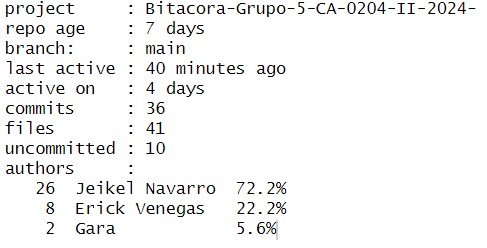
\includegraphics{imagenes/summary_1.jpeg}

}

\caption{Summary Bitacora 1}

\end{figure}%

\section{Anexo 3 (CHANGELOG Bitacora
2)}\label{anexo-3-changelog-bitacora-2}

\begin{figure}[H]

{\centering 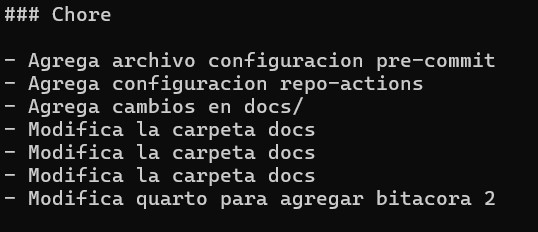
\includegraphics{imagenes/chore_2.jpeg}

}

\caption{Chore Bitacora 2}

\end{figure}%%
\begin{figure}[H]

{\centering 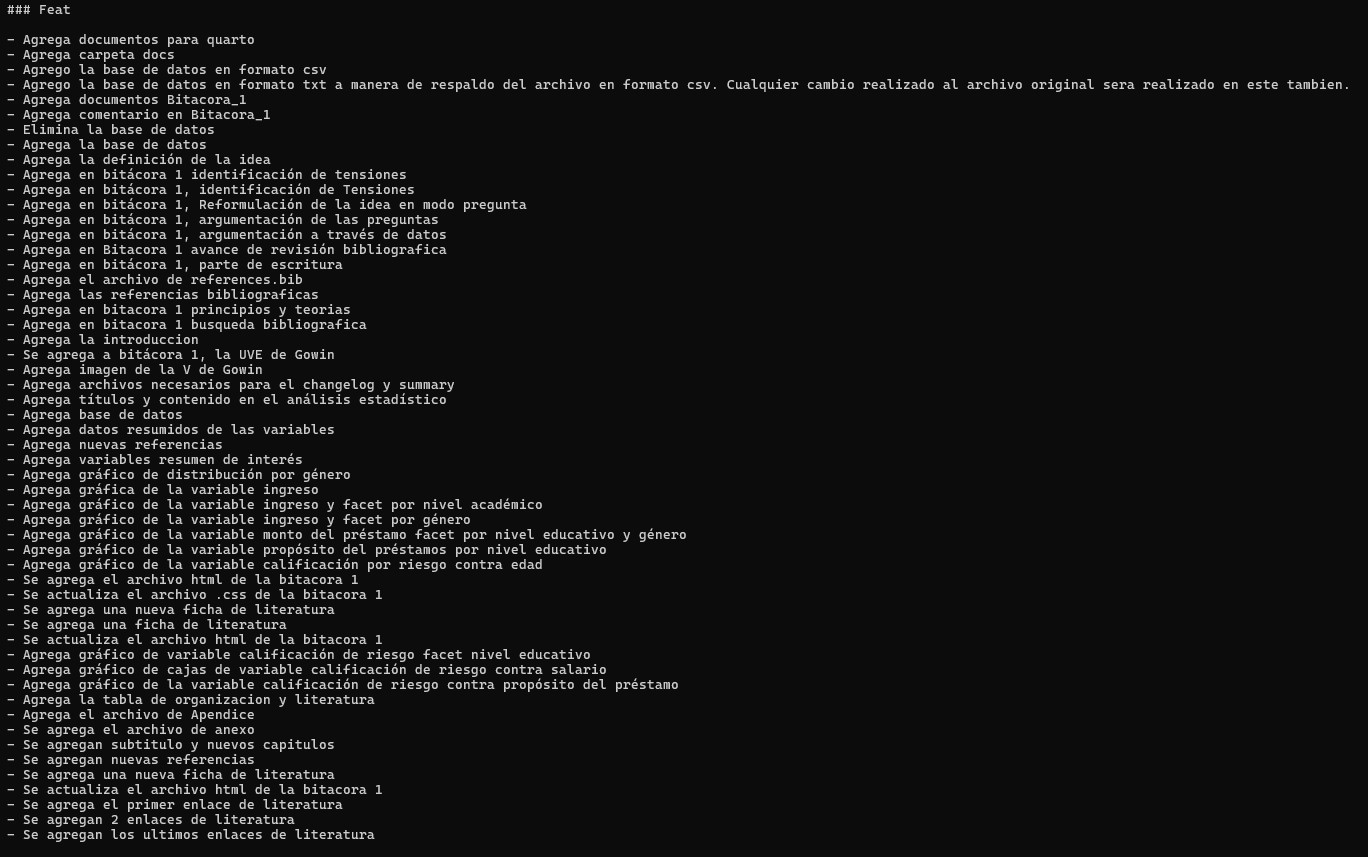
\includegraphics{imagenes/feat_2.jpeg}

}

\caption{Feat Bitacora 2}

\end{figure}%%
\begin{figure}[H]

{\centering 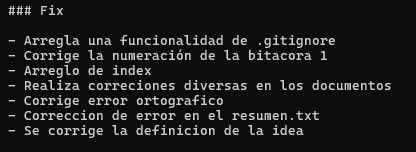
\includegraphics{imagenes/fix_2.jpeg}

}

\caption{Fix Bitacora 2}

\end{figure}%

\section{Anexo 4 (Participacion Bitacora
2)}\label{anexo-4-participacion-bitacora-2}

\begin{figure}[H]

{\centering 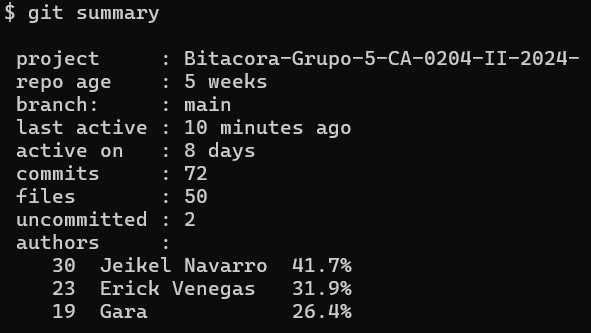
\includegraphics{imagenes/summary_2.jpeg}

}

\caption{Summary Bitacora 2}

\end{figure}%

\bookmarksetup{startatroot}

\chapter{Apendice}\label{apendice}

\section{Correcciones Bitácora 1}\label{correcciones-bituxe1cora-1}

La correccion más relevantes se detalla a continuación:

\begin{itemize}
\tightlist
\item
  \textbf{Corrección 1:} Se ha modificado la sección de definición de la
  idea para ajustarnos mejor a lo que se espera ser observado en la
  misma. Tal que, nos centramos más en definir claramente la idea de
  investigación, sin entrar en los detalles ni en dar el paso a paso de
  cómo se lleva la misma acabo. Por lo que, en esta sección, solo nos
  limitamos a exponer qué es lo que buscamos investigar y por qué es
  importante o relevante, dejando los aspectos metodológicos y el
  desarrollo de este para otras secciones.
\end{itemize}

\section{Sugerencias Bitácora 1}\label{sugerencias-bituxe1cora-1}

A partir del foro consideramos todas las sugerencias:

\begin{enumerate}
\def\labelenumi{\arabic{enumi}.}
\tightlist
\item
  \emph{El grupo podría ser más explícito en la metodología que usará y
  como abordará el objetivo general, esto lo observé en la sección de
  principios y teorías donde me parece que no tienen muy claro una
  teoría con la cual construir ideas relacionadas a la investigación.
  Hacen un buen análisis de la relación del tema de Riesgos con la
  Probabilidad y algunas teorías de valoración de riesgos financieros,
  pero podrían ser más explícitos en cual usarán y como la usarán.}
\end{enumerate}

\begin{itemize}
\tightlist
\item
  \textbf{Respuesta:} Gracias por la observación. Trataremos de que la
  metodología a utilizar quede un poco más explícita en la sección de
  principios y teorías, especialmente en relación con el análisis de la
  valoración de riesgos.
\end{itemize}

\begin{enumerate}
\def\labelenumi{\arabic{enumi}.}
\setcounter{enumi}{1}
\tightlist
\item
  \emph{Es crucial asegurar la validez de los datos utilizados, ya que
  estos deben reflejar con precisión las características reales de las
  personas con calificación crediticia. Aunque el enfoque del trabajo
  esté en el uso de herramientas de análisis de datos, es fundamental
  que la base de datos sea coherente con la realidad, dado que las
  conclusiones dependerán de la calidad de la información analizada.
  Además, sería recomendable incluir un título claro y descriptivo que
  refleje el objetivo principal del análisis.}
\end{enumerate}

\begin{itemize}
\tightlist
\item
  \textbf{Respuesta:} Agradecemos la sugerencia. Creemos que la base de
  datos que hemos escogido tiene una gran calidad o por lo menos visto
  desde un punto de vista académico, ya que está respaldada por el
  Instituto Tecnológico de Massachusetts (MIT). Adicional a eso, también
  hemos hecho una limpie de la base de datos para tratar de asegurarnos
  de aquellos datos tengan cierto grado de validez. A su vez, también
  hemos dejado mas en claro el título de la investigación.
\end{itemize}

\begin{enumerate}
\def\labelenumi{\arabic{enumi}.}
\setcounter{enumi}{2}
\tightlist
\item
  \emph{Considero que el proceso de selección de la pregunta final se
  pudo haber beneficiado de una argumentación más detallada para cada
  una de las opciones preliminares, especialmente haciendo una
  distinción más explícita entre los factores lógicos, éticos y
  emocionales que respaldan o cuestionan cada posible interrogante.
  Asimismo, es posible que la parte final de esta bitácora se pueda
  enriquecer con una mayor diversidad de fuentes, lo que ofrecería una
  perspectiva más amplia sobre los estudios que se han realizado
  previamente sobre el tema.}\\
\end{enumerate}

\begin{itemize}
\tightlist
\item
  \textbf{Respuesta:} Se tomará en cuenta su comentario. A la vez,
  estamos de acuerdo en que tal vez no llegamos a abarcar una gran
  variedad de fuentes, pero esto es debido a que la investigación se
  quiere mantener lo más aterrizada posible, de manera que no haya
  fuentes que sean innecesarias que a lo largo del trabajo no lleguen a
  tener relevancia. No obstante, hemos decido ampliar un poco más las
  fuentes, manteniendo el principio de no meter fuentes innecesarias.
\end{itemize}

\begin{enumerate}
\def\labelenumi{\arabic{enumi}.}
\setcounter{enumi}{3}
\tightlist
\item
  \emph{Sentí que la bitácora les quedó muy corta, la leí en poco tiempo
  y no entendí muy bien a qué querían llegar con los objetivos
  planteados. También siento que les faltó un poco más de referencias.
  La ventaja es que gracias a la naturaleza del tema esto se puede
  mejorar bastante fácil en las siguientes bitácoras.}
\end{enumerate}

\begin{itemize}
\tightlist
\item
  \textbf{Respuesta:} Agradecemos sus comentarios. A lo largo de la
  segunda bitácora vamos a profundizar más en los objetivos planteados,
  además, talvez la extensión de la primer bitácora se optó que fuese lo
  más concisa posible, tratando de que quedase lo más claro posible lo
  planteado en la misma, talque no se llegara a caer en redundancias.
  También como se menciona en otro comentario añadiremos más referencias
  que sean de utilidad para respaldar mejor el análisis.
\end{itemize}

\section{Referencias bibliográfica}\label{referencias-bibliogruxe1fica}

\phantomsection\label{refs}
\begin{CSLReferences}{1}{0}
\bibitem[\citeproctext]{ref-chicu2020}
Chicu, Dorina. 2020. {«La valoración del riesgo financiero»}. 2020.
\url{https://openaccess.uoc.edu/bitstream/10609/150126/1/LaValoracionDelRiesgoFinanciero.pdf}.

\bibitem[\citeproctext]{ref-edgar2022}
Edgar Apaza, César Condori, Samuel Cazorla. 2022. {«La Correlación de
Pearson o de Spearman en caracteres físicos y textiles de la fibra de
alpacas»}. 2022.
\url{http://www.scielo.org.pe/pdf/rivep/v33n3/1609-9117-rivep-33-03-e22908.pdf}.

\bibitem[\citeproctext]{ref-hadley2018}
Hadley Wickham, Garrett Grolemund. 2019. {«R for Data Science (2nd
ed.)»}. 2019.
\url{https://digitallibrary.tsu.ge/book/2019/september/books/R-for-Data-Science.pdf}.

\bibitem[\citeproctext]{ref-herrera2008}
Maria de los Ángeles Herrera, Juan Terán. 2024. {«Conceptualización del
riesgo de los mercados financieros»}. 2024.
\url{https://www.redalyc.org/pdf/900/90075920006.pdf}.

\bibitem[\citeproctext]{ref-palacios2012}
Palacios, Alberto. 2012. {«Calificación de riesgo: definición e
influencia en la última década»}. 2012.
\url{https://digibuo.uniovi.es/dspace/bitstream/handle/10651/4017/ACC-.pdf;jsessionid=723581A47435AFB6D2FEC05A70379F77?sequence=1}.

\bibitem[\citeproctext]{ref-maikol2024}
Solis, Maikol. 2024. {«Guía del curso: Herramienta para Ciencia de
Datos»}. 2024. \url{https://maikolsolis.com/libros/hpcd/}.

\end{CSLReferences}




\end{document}
